\part{Performance prediction through simulation}
\label{part:prediction}

The work presented in this part has been published at a conference\cite{cornebize:cluster19} and has been submitted
for publication in a journal\cite{cornebize:jpdc}. The content of this part is therefore a near-verbatim copy of these
articles. This work also directly follows my master thesis\cite{cornebize:master_thesis} whose main contribution is
summarized in chapter~\ref{chapter:prediction:emulation} for the sake of completeness.

\chapter{Related work}%
\label{chapter:prediction:related_work}

    %% We want to predict the performance of an application. It has several parameters, some relating to the problem size,
    %% others that control the behavior of the application.
    %%
    %% Criterions that may or may not be satisfied by a given approach:
    %% - extrapolation on the problem size
    %% - extrapolation on the behavior
    %% - prediction without having to make a full-scale real run
    %% - prediction for a hypothetical platform (what-if scenario)
    %% - efficiency
    %% - accuracy

    \section{Performance prediction}%
    \label{sec:performance_prediction}

        As discussed in Chapter~\ref{chapter:context}, researchers and engineers often need to make predictions about
        the performance of a given parallel application on a given platform. The reasons are diverse, it could be to
        compare several algorithms, to verify if the observed performance is as high as one could hope, or to estimate
        the gain they could get by upgrading their hardware.

        Depending on the exact needs of its user, such a prediction should fulfill several of these criterions:
        \begin{description}
            \item[Extrapolation on the problem size] Most of the applications can take as input problems of various
                size. The size may denote the number of particles in a physics simulator or the matrix rank in a linear
                algebra solver. The total duration will usually grow with the problem size. This creterion denotes
                whether the considered approach can predict the performance of the application for an unforeseen problem
                size.
            \item[Extrapolation on the configuration] It is often possible to tune the behavior of the application with
                some parameters, for instance to select the desired algorithm or the desired granularity. The reason is
                that the optimal parameter combination may depend on the hardware, the number of nodes, the problem
                size. This criterion designates if the approach can make predictions for an unforeseen parameter
                combination.
            \item[No full-scale real run] Some prediction methods will require at least one run of the application at
                the desired scale in terms of number of nodes. Note that this does not necessarily need to be done on
                the target platform.
            \item[Hypothetical platform] This criterion denotes the ability to study \emph{what-if scenarios}, \eg to
                predict the performance of the application on an hypothetical cluster with a higher network bandwidth
                than the ones available.
            \item[Efficiency] Some approaches have a much higher resource requirement than others. Several metrics can
                be considered: node-hours, time to solution, energy consumption, memory footprint.
            \item[Accuracy] While some predictions will only give an approximate trend, some others will be much more
                accurate, as close as a few percents, even in the presence of perturbations like network contention.
        \end{description}

        A first approach for estimating the performance of MPI applications is statistical modeling of the application
        as a whole\cite{hpl_prediction}.  By running the application several times with small and medium problem (of a
        few iterations of large problem sizes) and using simple linear regressions, it is possible to predict its
        makespan for larger sizes with an error of only a few percents and a relatively low cost.  Unfortunately, the
        predictions are limited to the same application configuration and studying the influence of the number of rows
        and columns of the virtual grid or of the broadcast algorithms requires a new model and new (costly) runs using
        the whole target machine.  Singh~\etal~\cite{Singh_2007} proposed the reverse approach. They fixed the problem
        size and sampled random parameter configurations to train a neural network. Again, this allowed them to make
        accurate predictions at a low cost, but it was not possible to predict the makespan with an unforeseen problem
        size. Furthermore, this kind of approaches inherently prevent to study what-if scenarios (\eg to evaluate what
        would happen if the network bandwidth was increased or if node heterogeneity was decreased) that are
        particularly useful when investigating potential performance improvements.

        Simulation provides the details and flexibility missing to such black-box modeling approach. Performance
        prediction of MPI applications through simulation has been widely studied over the last decades but two
        approaches can be distinguished in the literature: offline and online simulation.

        With the most common approach, \emph{offline simulation}, a trace of the application is first obtained on a real
        platform. This trace comprises sequences of MPI operations and CPU bursts and is given as an input to a
        simulator that implements performance models for the CPUs and the network to derive predictions. Researchers
        interested in finding out how their application reacts to changes to the underlying platform can replay the
        trace on commodity hardware at will with different platform models.  Most HPC simulators available today,
        notably BigSim\cite{bigsim_04}, Dimemas\cite{dimemas} and CODES\cite{CODES}, rely on this approach.  The main
        limitation of this approach comes from the trace acquisition requirement. Not only is a large machine required
        but the compressed trace of a few iterations of an MPI application can quickly reach a few hundred MB, making
        this approach quickly impractical\cite{suter}.  Worse, tracing an application provides only information about
        its behavior at the time of the run: slight modifications (\eg to communication patterns) may make the trace
        inaccurate. The behavior of simple applications (\eg \texttt{stencil}) can be extrapolated from small-scale
        traces\cite{scalaextrap,pmac_lspp13} but this fails if the execution is non-deterministic, \eg whenever the
        application relies on non-blocking communication patterns, which is unfortunately often the case.

        The second approach discussed in the literature is \emph{online simulation}.  Here, the application is executed
        (emulated) on top of a simulator that is responsible to determine when each process is run. This approach allows
        researchers to study directly the behavior of MPI applications but only a few recent simulators such as SST
        Macro\cite{sstmacro}, SimGrid/SMPI\cite{simgrid} and the closed-source xSim\cite{xsim} support it. To the best
        of our knowledge, only SST Macro and SimGrid/SMPI are mature enough to faithfully emulate an MPI application.
        This work relies on SimGrid as its performance models and its emulation capabilities seemed quite solid but the
        proposed developments would a priori also be possible with SST.  Note that the emulation described in
        chapter~\ref{chapter:prediction:emulation} should not be confused with the application
        skeletonization\cite{sst_skeleton} commonly used with SST. Skeletons are code extractions of the most important
        parts of a complex application whereas we only modify a few dozens of lines of the source code before emulating
        it with SMPI. Finally, it is important to understand that the proposed approach is intended to help studies at
        the level of the whole machine and application, not the influence of microarchitectural details as intended by
        MUSA\cite{musa_16}.

        The differences between these prediction approaches are summarized in
        Table~\ref{tab:prediction:state_of_the_art}.

        \begin{landscape}
            \newcommand{\yess}{\textcolor{green}{\cmark}}
            \newcommand{\nope}{\textcolor{red}{\xmark}}
            \begin{table}[htpb]
                \centering
                \caption{Summary of the different prediction approaches}
                \label{tab:prediction:state_of_the_art}
                \begin{tabular}{p{0.15\linewidth} | p{0.13\linewidth} p{0.13\linewidth} p{0.13\linewidth} p{0.13\linewidth}
                    p{0.13\linewidth} p{0.13\linewidth} }
                    Approach & Extrapolation on the problem size & Extrapolation on the configuration & No full-scale real
                    run & Hypothetical platform & Efficiency & Accuracy\\
                    \hline
                    \rowcolor{gray80} Big-O analysis          & \yess & \yess & \yess & \yess & \yess \yess & \nope\nope\\
                    \cite{hpl_prediction}   & \yess & \nope & \yess & \nope & \yess & \yess\\
                    \cite{Singh_2007}       & \nope & \yess & \nope & \nope & \yess & \yess\\
                    \hline
                    \rowcolor{gray80} Ideal off-line sim.     & \nope & \nope & \nope & \yess & \yess & \yess\\
                    BigSim\cite{bigsim_04}  & \\
                    Dimemas\cite{dimemas}   & \\
                    CODES\cite{CODES}       & \\
                    \hline
                    \rowcolor{gray80} Ideal on-line sim.      & \yess & \yess & \yess & \yess & \yess & \yess\\
                    xSim\cite{xsim}         & \\
                    SST\cite{sstmacro}      & \\
                    Simgrid\cite{simgrid}   & \yess & \yess & \yess & \yess & \yess & \yess\\
                \end{tabular}
            \end{table}
        \end{landscape}

    \section{Simgrid/SMPI}%
    \label{sec:simgrid_smpi}

        SimGrid\cite{simgrid} is a flexible and open-source simulation framework that was originally designed in 2000 to
        study scheduling heuristics tailored to heterogeneous grid computing environments but has later been extended to
        study cloud and HPC infrastructures. The main development goal for SimGrid has been to provide validated performance
        models particularly for scenarios making heavy use of the network.  Such a validation usually consists of comparing
        simulation predictions with results from real experiments to confirm or debunk network and application models.

        SMPI, a simulator based on SimGrid, has been developed and used to simulate unmodified MPI applications written in
        C/C++ or FORTRAN\cite{smpi}.
        The complex network optimizations done in real MPI implementations need to be considered when predicting the
        performance of MPI applications.  For instance, the "eager" and "rendez-vous" protocols are selected based on the
        message size, with each protocol having its own synchronization semantics, which strongly impact performance.  SMPI
        supports different performance modes through a generalization of the LogGPS model.  Another difficult issue is to
        model network topologies and contention. SMPI relies on SimGrid's communication models where each ongoing
        communication is represented as a whole (as opposed to single packets) by a \emph{flow}. Assuming steady-state,
        contention between active communications can then be modeled as a bandwidth sharing problem that accounts for
        non-trivial phenomena (\eg cross-traffic interference\cite{Velho_TOMACS13}). If needed, communications that start or
        end trigger a re-computation of the bandwidth share.  In this fluid model, the time to simulate a message passing
        through the network is independent of its size, which is advantageous for large-scale applications frequently
        sending large messages and orders of magnitude faster than packet-level simulation.  SimGrid does not model
        transient phenomena incurred by the network protocol but accounts for network topology and heterogeneity. Special
        attention to the modeling of collective communication algorithms has also been paid in SMPI, but this is of little
        significance in this article as HPL ships with its own implementation of collective operations.

        SMPI maps every MPI rank of the application onto a lightweight simulation thread. These threads are then run one at
        a time, \ie in mutual exclusion.  Every time a thread enters an MPI call, SMPI takes control and the time that was
        spent computing (isolated from the other threads) since the previous MPI call is injected into the simulator as a
        virtual delay.  This time may be scaled up or down depending on the speed of the simulated machine with respect to
        the simulation machine.
        Recent results report consistent performance predictions within a few percent for standard benchmarks on small-scale
        clusters (up to \(12\times12\) cores \cite{heinrich:hal-01523608} and up to \(128\times1\) cores \cite{smpi}). In
        this thesis, I validate this approach at a much larger scale with HPL, whose emulation comes with at least two
        challenges:
        \begin{itemize}
        \item The time-complexity of the algorithm is \(\Theta(N^3)\) and \(\Theta(N^2)\) communications are performed, with
            \(N\) being very large. The execution on the Stampede cluster took roughly two hours on \Num{6006}~compute
            nodes. Using only a single node, a naive emulation of HPL at the scale of the Stampede run would take about
            500 days if perfect scaling was reached.
        \item The tremendous memory consumption and amount of memory accesses need to be drastically reduced.
        \end{itemize}

\chapter{High Performance Linpack}%
\label{chapter:prediction:hpl}

    \section{The benchmark}%
    \label{sec:hpl:benchmark}

        \begin{figure}[ht]
            \newcommand{\mykwfn}[1]{{\textbf{\textsf{#1}}}}%
            \SetAlFnt{\textsf}%
            \SetKwSty{mykwfn}%
            \SetKw{KwStep}{step}%
            \centering
            \begin{minipage}[m]{0.5\linewidth}
                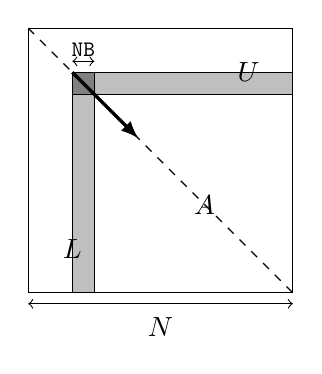
\begin{tikzpicture}[scale=0.28]
                    \draw (0, 0) -- (0, 12) -- (12, 12) -- (12, 0) -- cycle;
                    \foreach \i in {2}{
                        \draw [fill=lightgray] (\i, 0) -- (\i, 12-\i) -- (12, 12-\i) -- (12, 0) -- cycle;
                        \draw [fill=gray] (\i, 12-\i) -- (\i, 12-\i-1) -- (\i+1, 12-\i-1) -- (\i+1, 12-\i) -- cycle;
                        \draw[very thick, -latex] (\i,12-\i) -- (\i+2,12-\i-2);
                        \draw[<->] (\i, 12-\i+0.5) -- (\i+1, 12-\i+0.5) node [pos=0.5, yshift=+0.15cm] {\scalebox{.8}{\texttt{NB}}};
                    }
                    \foreach \i in {3}{
                        \draw [fill=white] (\i, 0) -- (\i, 12-\i) -- (12, 12-\i) -- (12, 0) -- cycle;
                        \draw (\i,12-\i) -- (\i,0);
                        \draw[very thick, -latex] (\i,12-\i) -- (\i+2,12-\i-2);
                    }
                    \draw[dashed] (0, 12) -- (12, 0);
                    \node(L) at (2, 2) {\ensuremath{\boldsymbol{L}}};
                    \node(U) at (10, 10) {\ensuremath{\boldsymbol{U}}};
                    \node(A) at (8, 4) {\ensuremath{\boldsymbol{A}}};
                    \draw[<->] (0, -0.5) -- (12, -0.5) node [pos=0.5, yshift=-0.3cm] {$N$};
                \end{tikzpicture}
            \end{minipage}%
            \begin{minipage}[m]{0.5\linewidth}
                \begin{algorithm}[H]
                    \DontPrintSemicolon
                    allocate and initialize $A$\;
                    \For{$k=N$ \KwTo $0$ \KwStep \texttt{NB}}{
                        allocate the panel\;
                        factor the panel\;
                        broadcast the panel\;
                        update the sub-matrix;
                    }
                    \caption{HPL}
                    \label{algo:hpl}
                \end{algorithm}
            \end{minipage}
            \caption{Overview of High Performance Linpack}
            \label{fig:hpl_overview}
        \end{figure}

        In this work, we use the freely-available reference-implementation of HPL\cite{hpl}, which relies on MPI.  HPL
        implements a matrix factorization based on a right-looking variant of the LU factorization with row partial pivoting
        and allows multiple look-ahead depths. The principle of the factorization is depicted in
        Figure\ref{fig:hpl_overview}. It consists of a series of panel factorizations followed by an update of the trailing
        sub-matrix.  HPL uses a two-dimensional block-cyclic data distribution of $A$ and implements several custom MPI
        collective communication algorithms to efficiently overlap communications with computations.
        The main parameters of HPL are:
        \begin{itemize}
            \item \texttt{N} is the order of the square matrix $A$.
            \item \texttt{NB} is the \emph{blocking factor}, \ie the granularity at which HPL operates when panels are
                distributed or worked on.
            \item \texttt{P} and \texttt{Q} denote the number of process rows and the number of process columns,
                respectively.
            \item \texttt{RFACT} determines the panel factorization algorithm. Possible values are Crout, left- or
                right-looking.
            \item \texttt{SWAP} specifies the swapping algorithm used while pivoting. Two algorithms are available: one
                based on \emph{binary exchange} (along a virtual tree topology) and the other one based on a
                \emph{spread-and-roll} (with a higher number of parallel communications). HPL also provides a panel-size
                threshold triggering a switch from one variant to the other.
            \item \texttt{BCAST} sets the algorithm used to broadcast a panel of columns over the process columns. Legacy
                versions of the MPI standard only supported non-blocking point-to-point communications, which is why HPL
                ships with in total 6 self-implemented variants to overlap the time spent waiting for an incoming panel with
                updates to the trailing matrix: \texttt{ring}, \texttt{ring-modified}, \texttt{2-ring},
                \texttt{2-ring-modified}, \texttt{long}, and \texttt{long-modified}. The \texttt{modified} versions
                guarantee that the process right after the root (\ie the process that will become the root in the next
                iteration) receives data first and does not further participate in the broadcast. This process can thereby
                start working on the panel as soon as possible. The \texttt{ring} and \texttt{2-ring} versions each
                broadcast along the corresponding virtual topologies while the \texttt{long} version is a \emph{spread and
                roll} algorithm where messages are chopped into \texttt{Q} pieces. This generally leads to better bandwidth
                exploitation. The \texttt{ring} and \texttt{2-ring} variants rely on \texttt{MPI\_Iprobe}, meaning they
                return control if no message has been fully received yet, hence facilitating partial overlap of
                communication with computations.  In HPL 2.1 and 2.2, this capability has been deactivated for the
                \texttt{long} and \texttt{long-modified} algorithms. A comment in the source code states that some machines
                apparently get stuck when there are too many ongoing messages.
            \item \texttt{DEPTH} controls how many iterations of the outer loop can overlap with each other.
        \end{itemize}

        The sequential complexity of this factorization is \[\mathrm{flop}(N) = \frac{2}{3}N^3 + 2N^2 + \landauO(N)\] where $N$ is
        the order of the matrix to factorize. The time complexity can be approximated by \[T(N) \approx
        \frac{\left(\frac{2}{3}N^3 + 2N^2\right)}{P\cdot{}Q\cdot{}w} + \Theta((P+Q)\cdot{}N^2)\] where $w$ is the flop rate
        of a single node and the second term corresponds to the communication overhead which is influenced by the network
        capacity and the previously listed parameters (\texttt{RFACT}, \texttt{SWAP}, \texttt{BCAST},
        \texttt{DEPTH}, \ldots) and is very difficult to predict.

    \section{Typical runs on a supercomputer}%
    \label{sec:hpl:typical_runs}

        Although the TOP500 reports precise information about the core count,
        the peak performance and the effective performance, it provides almost
        no information on how (software versions, HPL parameters, etc.) this
        performance was achieved. Some colleagues agreed to provide us with
        the HPL configuration they used and the output they submitted for
        ranking (see Table\ref{fig:typical_run}).
        In June 2013, the Stampede supercomputer at TACC was ranked
        6th in the TOP500 by achieving \NSI{5168.1}{\tera\flops}. In November
        2017, the Theta supercomputer at ANL was ranked 18th with a performance of \NSI{5884.6}{\tera\flops}
        but required a 28-hour run on the
        whole machine. Finally, we ran HPL ourselves on a Grid'5000 cluster
        named Dahu whose software stack could be fully controlled.

        \begin{table}[hb]
            \caption{Typical runs of HPL}
            \label{fig:typical_run}
            \scalebox{.9}{\begin{tabular}{l|lll}
                \multicolumn{1}{l|}{} & Stampede@TACC & Theta@ANL & Dahu@G5K\\
                \hline
                \texttt{Rpeak}     & \NSI{8520.1}{\tera\flops} & \NSI{9627.2}{\tera\flops} & \NSI{62.26}{\tera\flops}              \\
                $N$         & \Num{3875000}                & \Num{8360352}                & \Num{500000}            \\
                \texttt{NB}        & \Num{1024}                    & 336                      & 128                \\
                $P\times Q$             & 77$\times$78                  & 32$\times$101                 & 32$\times$32            \\
                \texttt{RFACT}     & Crout                    & Left                     & Right              \\
                \texttt{SWAP}      & Binary-exch.             & Binary-exch.             & Binary-exch.       \\
                \texttt{BCAST}     & Long modified            & 2 Ring modified          & 2 Ring             \\
                \texttt{DEPTH}     & 0                        & 0                        & 1                  \\
                \hline
                \texttt{Rmax}      & \NSI{5168.1}{\tera\flops} & \NSI{5884.6}{\tera\flops} & \NSI{24.55}{\tera\flops}              \\
                Duration   & 2 hours                  & 28 hours                 & 1 hour             \\
                Memory    & \NSI{120}{\tera\byte}     & \NSI{559}{\tera\byte}     & \NSI{2}{\tera\byte} \\
                MPI ranks & 1/node                & 1/node                   & 1/core             \\
            \end{tabular}}
        \end{table}


        The performance typically achieved by supercomputers (\texttt{Rmax}) needs to be compared to the much larger
        peak performance (\texttt{Rpeak}). This difference can be attributed to the node usage, to the MPI library, to
        the network topology that may be unable to deal with the intense communication workload, to load imbalance among
        nodes (\eg due to a defect, system noise, \ldots), to the algorithmic structure of HPL, etc. All these factors
        make it difficult to know precisely what performance to expect without running the application at scale.  It is
        clear that due to the level of complexity of both HPL and the underlying hardware, simple performance models
        (analytic expressions based on $N, P, Q$ and estimations of platform characteristics) may be able to provide
        trends but can by no means accurately predict the performance for each configuration (\eg consider the exact
        effect of HPL's six different broadcast algorithms on network contention). Additionally, these expressions do
        not allow engineers to improve the performance through actively identifying performance bottlenecks.  For
        complex optimizations such as partially non-blocking collective communication algorithms intertwined with
        computations, a very faithful modeling of both the application and the platform is required. One goal of this
        thesis was to simulate systems at the scale of Stampede. Given the scale of this scenario (3,785~steps on
        6,006 nodes in two hours), detailed simulations quickly become intractable without significant effort.

\chapter{Emulating HPL at large scale}%
\label{chapter:prediction:emulation}

    In this chapter, we present the changes to SimGrid and HPL that were required for a scalable simulation.  The
    experiments were done using a single core from nodes of the Nova cluster provided by the Grid'5000
    testbed\cite{grid5000} (\NSI{32}{\giga\byte} of RAM, two 8-core Intel Xeon E5-2620 v4 CPUs, Debian Stretch OS
    (Linux 4.9)).

    %% TODO
    %% - On remplace les appels à dgemm par des régressions linéaires
    %%   (expliquer ce qu'il y avait avant, i.e. pas grand chose)
    %% - execute -> sleep (même si du coup, ça marche plus pour l'énergie,
    %%   pour que ça marche pour l'énergie, il faut revoir la création de
    %%   plate-forme et le plugin énergie)

    \section{Speeding Up the Emulation}
    \label{sec:speeding_emulation}

        \subsection{Compute Kernel Modeling}
            \begin{figure}[htb]
                \centering
                \subfigure[Non-intrusive macro replacement with a very simple computation model.\label{fig:macro_simple}]{
                    \begin{minipage}[b]{\linewidth}
                        \lstset{frame=bt,language=C,numbers=none,escapechar=|}\lstinputlisting{img/prediction/emulating/HPL_dgemm_macro_simple.c}
                    \end{minipage}}\vspace{-1em}
                \subfigure[Gain in terms of simulation time.\label{fig:kernel_sampling}]{
                    \begin{minipage}[b]{\linewidth}
                        
\includegraphics[width=\linewidth,page=2]{img/prediction/emulating/kernel_modeling.pdf}
                    \end{minipage}}%\vspace{-1em}
                \caption{Replacing the calls to computationally expensive functions by a model allows to emulate HPL at
                a larger scale.}\vspace{-1em}
            \end{figure}

            HPL heavily relies on BLAS kernels such as \dgemm (for matrix-matrix multiplication) or \texttt{dtrsm}
            (for solving an  \(A\cdot x=b\) equation). The analysis of an HPL simulation with \(64\) processes and a very
            small matrix of order \Num{30000} showed that about \(\NSI{96}{\percent}\) of the time is spent in these two
            kernels. Since the output of these kernels does not influence the control flow, simulation time can be reduced
            by substituting \dgemm and \texttt{dtrsm} function calls with a performance model of the respective
            kernel.
            Skipping kernels renders the content of some variables invalid but in simulation, only the behavior of the
            application and not the correctness of computation results are of concern.  Figure\ref{fig:macro_simple} shows
            an example of this macro-based mechanism that allows to keep HPL code modifications to an absolute minimum. The
            \texttt{(1.029e-11)} value represents the inverse of the flop rate for this compute kernel and was obtained
            through calibration. The estimated time of the kernel is calculated based on the given parameters and passed on
            to \texttt{smpi\_execute\_benched} that advances the clock of the executing rank by this estimate.  The effect
            on the simulation time for a small scenario is depicted in Figure\ref{fig:kernel_sampling}. This modification
            speeds up the simulation by orders of magnitude. The precision of the simulation will be investigated in more
            details in the next chapter but it can already be observed that this simple kernel model leads to a sound,
            albeit slightly more optimistic, estimation of the performance.

            In addition to the main compute kernels, a profiling of the code allowed to identify seven other BLAS functions
            as computationally expensive enough to justify a specific handling: \texttt{dgemv}, \texttt{dswap},
            \texttt{daxpy}, \texttt{dscal}, \texttt{dtrsv}, \texttt{dger} and \texttt{idamax}. Similarly, a significant
            amount of time was spent in fifteen functions implemented in HPL: \texttt{HPL\_dlaswp*N},
            \texttt{HPL\_dlaswp*T}, \texttt{HPL\_dlacpy} and \texttt{HPL\_dlatcpy}.  All these functions are called during
            the LU factorization and hence impact the performance measured by HPL; however, because of the removal of the
            \dgemm and \texttt{dtrsm} computations, they all operate on bogus data and hence also produce bogus
            data. They have been handled similarly to \dgemm and \texttt{dtrsm}, through performance models and
            macro substitution, which speeds up the simulation by an additional factor of \(3\) to \(4\) on small
            (\(N=\Num{30000}\)) and even more on large scenarios.

        \subsection{Specific Adjustments}
            HPL uses pseudo-randomly generated matrices that are setup every time HPL is executed. This initialization, just
            like the factorization correctness verification at the end of the run, is not considered in the reported
            performance and can therefore be safely skipped.  Note that HPL implements an LU factorization with partial
            pivoting, which requires a special treatment of the \texttt{idamax} function that returns the index of the first
            element equaling the maximum absolute value. Although the cost of this function was ignored as well, its return
            value was has been set to a random (but controlled) value to make the simulation unbiased (but fully
            deterministic).

    \section{Scaling Down Memory Consumption}
        The largest two allocated data structures in HPL are the input matrix \texttt{A} (with a size of typically
        several \si{\giga\byte} per process) and the \texttt{panel} which contains information about the sub-matrix
        currently being factorized. This sub-matrix typically occupies a few hundred \si{\mega\byte} per process.
        Unfortunately, when emulating an application with SMPI, all MPI processes are run within the same simulation
        process on a single node and the memory consumption of the simulation can therefore quickly reach several
        \si{\tera\byte} of RAM.  Yet, as we no longer operate on real data, storing the whole input matrix \(A\) is
        needless. However, since only a minimal portion of the code was modified, some functions may still read or write
        some parts of the matrix.  It is thus not possible to simply remove the memory allocations of large data
        structures. SMPI provides the \texttt{SMPI\_SHARED\_MALLOC} (\texttt{SMPI\_SHARED\_FREE}) macro to replace calls
        to \texttt{malloc} (\texttt{free}). They indicate that some data structures can safely be shared between
        processes and that the data they contain is not critical for the execution (\eg an input matrix) and that it may
        even be overwritten. \texttt{SMPI\_SHARED\_MALLOC} works as follows (see
        Figure\ref{fig:global_shared_malloc}): a single block of physical memory (of default size \NSI{1}{\mega\byte})
        for the whole execution is allocated and shared by all MPI processes.  A range of virtual addresses
        corresponding to a specified size is reserved and cyclically mapped onto the previously obtained physical
        address.  This mechanism allows most applications to obtain a nearly constant memory footprint, regardless of
        the size of the actual allocations.

        \tikzset{draw half paths/.style 2 args={%
          % From https://tex.stackexchange.com/a/292108/71579
            decoration={show path construction,
              lineto code={
                \draw [#1] (\tikzinputsegmentfirst) --
                   ($(\tikzinputsegmentfirst)!0.5!(\tikzinputsegmentlast)$);
                \draw [#2] ($(\tikzinputsegmentfirst)!0.5!(\tikzinputsegmentlast)$)
                  -- (\tikzinputsegmentlast);
              }
            }, decorate
        }}
        \tikzstyle{switch}=[draw, circle, minimum width=1cm, minimum height = 1cm]
        \tikzstyle{compute}=[draw, rectangle, minimum width=0.5cm, minimum height = 0.5cm, node distance=0.5cm]
        \tikzstyle{base}=[ellipse, minimum width=2cm, minimum height = 0.5cm, node distance = 0.5cm]
        \tikzstyle{bigswitch}=[base, draw]
        \begin{figure}[t]%[htbp]
            \vspace{-1em}\centering
            \begin{tikzpicture}[yscale=0.5, scale=0.7]
                \pgfmathtruncatemacro{\size}{4}
                \pgfmathtruncatemacro{\width}{2}
                \pgfmathtruncatemacro{\sizem}{\size-1}
                \pgfmathtruncatemacro{\smallbasex}{4}
                \pgfmathtruncatemacro{\smallbasey}{\size/2}
                \pgfmathtruncatemacro{\smallstopx}{\smallbasex+\width}
                \pgfmathtruncatemacro{\smallstopy}{\smallbasey+1}
                \foreach \i in {0,\sizem}{
          	        \pgfmathtruncatemacro{\j}{\i+1}
          	        \draw (0, \i) -- (0, \j);
          	        \draw (\width, \i) -- (\width, \j);
          	        \draw[dotted] (0, \i) -- (\width, \i);
          	        \draw[dotted] (0, \j) -- (\width, \j);
          	    }
          	    \draw[dashed] (0, 1) -- (0, \sizem);
          	    \draw[dashed] (\width, 1) -- (\width, \sizem);
          	    \draw (0, 0)     -- (\width, 0);
          	    \draw (0, \size) -- (\width, \size);
                \draw (\smallbasex,\smallbasey) -- (\smallstopx,\smallbasey) -- (\smallstopx,\smallstopy) --
                (\smallbasex,\smallstopy) -- cycle;
                \foreach \i in {0,\sizem}{
          	        \pgfmathtruncatemacro{\j}{\i+1}
          	        \draw[dotted] (\width, \i) -- (\smallbasex, \smallbasey);
          	        \draw[dotted] (\width, \j) -- (\smallbasex, \smallstopy);
          	        \pgfmathsetmacro{\xleft}{\width}
          	        \pgfmathsetmacro{\xright}{\smallbasex}%{\width/2.0+\smallbasex/2.0}
          	        \pgfmathsetmacro{\yleft}{\i + 0.5}
          	        \pgfmathsetmacro{\yright}{\smallbasey + 0.5}
          	        \path [draw half paths={solid, -latex}{draw=none}]  (\xleft, \yleft) -- (\xright, \yright);
          	    }
                \draw[decorate,line width=1pt,decoration={brace,raise=0.2cm}] (0, 0) -- (0, \size) node [pos=0.5,
                xshift=-1cm] {virtual};
                \draw[decorate,line width=1pt,decoration={brace,mirror,raise=0.2cm}] (\smallstopx, \smallbasey) --
                (\smallstopx, \smallstopy) node [pos=0.5, xshift=1.2cm] {physical};
            \end{tikzpicture}
            \caption{\label{fig:global_shared_malloc}SMPI shared malloc mechanism: large area of virtual memory are
            mapped onto the same physical pages.}\vspace{2em}

           \centering
           {\begin{minipage}{1.0\linewidth}
            \subfigure[Structure of the panel in HPL.\label{fig:panel_structure}]{\small
                \begin{minipage}[b]{\linewidth}\centering
                    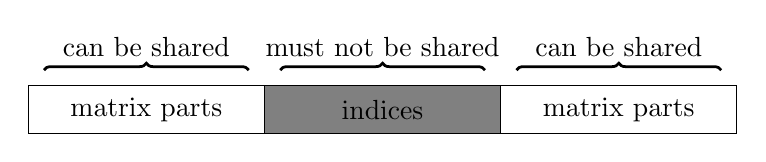
\begin{tikzpicture}[yscale=.6,scale=1]
                        \draw [fill=gray] (3, 2) -- (6, 2) -- (6, 3) -- (3, 3) -- cycle;
                        \draw (0, 2) -- (9, 2) -- (9, 3) -- (0, 3) -- cycle;
                        \draw[dashed] (3, 2) -- (3, 3);
                        \draw[dashed] (6, 2) -- (6, 3);
                        \node(1) at (1.5, 2.5) {matrix parts};
                        \node(2) at (4.5, 2.5) {indices};
                        \node(3) at (7.5, 2.5) {matrix parts};
                        \draw[decorate,line width=1pt,decoration={brace,raise=0.2cm}] (0.2, 3) -- (2.8, 3) node
                        [pos=0.5, yshift=0.5cm] {can be shared};
                        \draw[decorate,line width=1pt,decoration={brace,raise=0.2cm}] (6.2, 3) -- (8.8, 3) node
                        [pos=0.5, yshift=0.5cm] {can be shared};
                        \draw[decorate,line width=1pt,decoration={brace,raise=0.2cm}] (3.2, 3) -- (5.8, 3) node
                        [pos=0.5, yshift=+0.5cm] {must not be shared};
                    \end{tikzpicture}
                \end{minipage}}\vspace{-1em}
            \subfigure[Reusing panel allocation from an iteration to another.\label{fig:panel_reuse}]{\small
                \begin{minipage}[b]{\linewidth}\centering
                    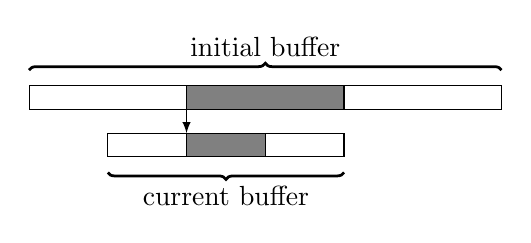
\begin{tikzpicture}[yscale=.6,scale=1]
                        \draw [fill=gray] (2, 1) -- (4, 1) -- (4, 1.5) -- (2, 1.5) --cycle;
                        \draw (0, 1) -- (6, 1) -- (6, 1.5) -- (0, 1.5) -- cycle;
                        \draw[dashed] (2, 1) -- (2, 1.5);
                        \draw[dashed] (4, 1) -- (4, 1.5);

                        \draw [fill=gray] (2, 0) -- (3, 0) -- (3, .5) -- (2, .5) --cycle;
                        \draw (1, 0) -- (4, 0) -- (4, .5) -- (1, .5) -- cycle;
                        \draw[dashed] (2, 0) -- (2, .5);
                        \draw[dashed] (3, 0) -- (3, .5);

                        \draw[-latex] (2, 1) -- (2, .5);
                        \draw[decorate,line width=1pt,decoration={brace,raise=0.2cm}] (0, 1.5) -- (6, 1.5) node
                        [pos=0.5, yshift=0.5cm] {initial buffer};
                        \draw[decorate,line width=1pt,decoration={brace,raise=0.2cm, mirror}] (1, 0) -- (4, 0) node
                        [pos=0.5, yshift=-0.5cm] {current buffer};
                    \end{tikzpicture}
                \end{minipage}%
            }%
            \end{minipage}}%\vspace{-1em}
            \caption{Panel structure and allocation strategy.\label{fig:panel}}\vspace{-1em}
        \end{figure}

        Although using the default \texttt{SHARED\_MALLOC} mechanism works flawlessly for \texttt{A}, a more careful
        strategy needs to be used for the \texttt{panel}, which is an intricate data structure with both \texttt{int}s
        (accounting for matrix indices, error codes, MPI tags, and pivoting information) and \texttt{double}s
        (corresponding to a copy of a sub-matrix of \texttt{A}). To optimize data transfers, HPL flattens this structure
        into a single allocation of \texttt{double}s (see Figure\ref{fig:panel_structure}). Using a fully shared memory
        allocation for the \texttt{panel} therefore leads to index corruption that results in classic invalid memory
        accesses. Since \texttt{int}s and \texttt{double}s are stored in non-contiguous parts of this flat allocation,
        it is therefore essential to have a mechanism that preserves the process-specific content. We have thus
        introduced the \texttt{SMPI\_PARTIAL\_SHARED\_MALLOC} macro that allows us to specify which ranges of the
        allocation should be preserved (\ie are private to each process) and which ones may be corrupted (\ie are shared
        between processes).  For a matrix of order \(40,000\) and \(64\) MPI processes, memory consumption decreases
        with this approach from about \NSI{13.5}{\giga\byte} to less than \NSI{40}{\mega\byte}.

        Another HPL specific optimization is related to the systematic allocation and deallocation of panels in each
        iteration, with the size of the panel strictly decreasing from iteration to iteration. As explained above,
        the partial sharing of panels requires many calls to \texttt{mmap} and introduces an overhead that makes these
        repeated allocations / frees a bottleneck. Since the very first allocation can fit all subsequent panels, we
        modified this allocation mechanism so that SMPI can reuse panels as much as possible from an iteration to an
        other (see Figure\ref{fig:panel_reuse}). Even for a very small matrix of order \(40,000\) and \(64\) MPI
        processes, the simulation time decreases from \NSI{20.5}{\sec} to \NSI{16.5}{\sec}.  The number of page faults
        decreased from \(2\) million to \(0.2\) million, confirming the devastating effect these
        allocations/deallocations would have at scale.

        The next three optimizations are not specific to HPL.  We leveraged the information on which memory area is
        private, shared or partially shared to improve the overall performance.  By making SMPI internally aware of the
        memory's visibility, it can now avoid calling \texttt{memcopy} when large messages containing shared segments
        are sent from one MPI rank to another.  For fully private or partially shared segments, SMPI identifies and
        copies only those parts that are process-dependent (private) into the corresponding buffers on the receiver
        side.  HPL simulation times and memory consumption were considerably improved in our experiments because the
        \texttt{panel} is the most frequently transferred data structure but only a small part of it is actually
        private.

        As explained above, SMPI maps MPI processes to threads of a single process, effectively folding them into the
        same address space.  Consequently, global variables in the MPI application are shared between threads unless
        these variables are \emph{privatized} and the simulated MPI ranks thus isolated from each other. Several
        technical solutions are possible to handle this issue\cite{smpi}. The default strategy in SMPI consists in
        making a copy of the \texttt{data} segment (containing all global variables) per MPI rank at startup and, when
        context switching to another rank, to remap the \texttt{data} segment via \texttt{mmap} to the private copy of
        that rank.  SMPI also implements another mechanism relying on the \texttt{dlopen} function that allows to load
        several times the \texttt{data} segment in memory and to avoid costly calls to \texttt{mmap} (and subsequent
        cache flush) when context switching. For a matrix of order \Num{80000} and \(32\) MPI processes, the number of
        minor page faults drops from \Num{4412047} (with \texttt{mmap}) to \Num{6880} (with \texttt{dlopen}), which
        results in a reduction of system time from \NSI{10.64}{\sec} (out of \NSI{51.47}{\sec}) to \NSI{2.12}{\sec}.

        Finally, for larger matrix orders (\ie \(N\) larger than a few hundred thousands), the performance of the
        simulation quickly deteriorates as the memory consumption rises rapidly. Indeed, folding the memory reduces the
        \emph{physical} memory usage. The \emph{virtual} memory, on the other hand, is still allocated for every process
        since the allocation calls are still executed.  Without a reduction of allocated virtual addresses, the page
        table rapidly becomes too large for a single node. Thankfully, the x86-64 architecture supports several page
        sizes, such as the \emph{huge pages} in Linux. Typically, these pages are around \NSI{2}{\mebi\byte} (instead of
        \NSI{4}{\kibi\byte}), which reduces drastically the page table size. For example, for a matrix of order
        \(N=4,000,000\), it shrinks from \NSI{250}{\giga\byte} to \NSI{0.488}{\giga\byte}.

    \section{Scalability Evaluation}
        \begin{figure}[t]
            \centering
            
\includegraphics[width=\linewidth,page=2]{./img/prediction/emulating/scalability_plot_size.pdf}
            \caption{Time complexity and memory consumption are linear in the number of processes but remain mildly
            quadratic with matrix rank.}
            \label{fig:hpl_scalability}
        \end{figure}

        The main goal of the previous optimizations is to reduce the complexity from \(\Theta(N^3) +
        \Theta(N^2\cdot{}P\cdot{}Q)\) to something more reasonable.  The \(\Theta(N^3)\) was removed by skipping most
        computations.  Ideally, since there are \(N/NB\) iterations (steps), the complexity of simulating one step
        should be decreased to something independent of \(N\). SimGrid's fluid models, used to simulate communications,
        do not depend on \(N\). Therefore, the time to simulate a step of HPL should mostly depend on \(P\) and \(Q\).
        Yet, some memory operations on the panel that are related to pivoting are intertwined in HPL with collective
        communications, meaning that it is impossible to get rid of the \(\landauO(N)\) complexity without modifying HPL more
        profoundly.

        To evaluate the efficiency of our proposal, we conduct a first evaluation on a non-existing but Stampede
        resembling platform comprising 4,096 nodes interconnected through a fat-tree topology.
        We run simulations with \Num{512}, \Num{1024}, \Num{2048} or \Num{4096} MPI ranks and with matrices of orders
        \Num{5e5}, \Num{1e6}, \Num{2e6} or \Num{4e6}. All other HPL parameters are similar to the ones of the original
        Stampede scenario.  The impact of the matrix order on total makespan and memory is illustrated in
        Figure\ref{fig:hpl_scalability}.  With all previously described optimizations enabled, the longest simulation
        took close to \(47\) hours and consumed \NSI{16}{\giga\byte} of memory whereas the shortest one took \(20\)
        minutes and \NSI{282}{\mega\byte} of memory.

\chapter{Modeling HPL kernels and communications}%
\label{chapter:prediction:modeling}

    As explained in chapter~\ref{chapter:prediction:emulation}, HPL spends most of its computation time in a dozen specific
    functions for which a performance model has to be designed. Most compute kernels have several parameters from which
    a very simple model can generally easily be identified (\eg proportional to the product of the parameters) but
    refinements including the individual contribution of each parameter as well as the spatial and temporal variability
    of the operation are also possible. Likewise, communications between two nodes are mostly linear in message size but
    the actual performance can wildly vary depending on the range of the message size as MPI switches from one
    protocol to another whenever needed. In this chapter we first introduce some notations to describe the complexity of
    the models we have investigated. We then briefly compare the prediction of these models with individual measurements
    of both computations and communications to illustrate the importance of the model complexity.

    \section{Modeling notations}%

        We denote as \(T\) the duration of an operation with parameters \(M\), \(N\), \(K\) (in the case of the
        \dgemm operation, these parameters describe the geometry of the input matrices). We first consider the
        three following modeling options:
        \begin{itemize}
            \item Modeling option \model{0}: For simple and stable compute kernels, the duration can be modeled as a
                constant duration independent of the input parameters, \ie \(T \sim \alpha\), where \(\alpha\) is
                estimated through the sample average of the duration of the operation (or simply 0 if the kernel is
                negligible) .
            \item Modeling option \model{1}: A simple combination of the parameters (\eg \(S=M.N.K\)) may be the primary
                factor driving the performance of the operation. Then \(T \sim \alpha.S ~(+ \beta)\) and \(\alpha\) and
                \(\beta\) can be estimated through a classical least-square linear regression.
            \item Modeling option \model{2}: When the behavior of the operation is complex or requires a faithful
                modeling over the full range of input parameters, a full polynomial model is required, \ie \(T \sim
                \alpha.M.N.K + \beta.M.N + \gamma.N.P + \dots \) Again, the \(\alpha,\beta,\gamma,\dots\) can be
                estimated through a classical least-square linear regression.
        \end{itemize}
        There are two situations where more elaborate variations need to be considered:
        \begin{itemize}
            \item Whenever the platform is slightly heterogeneous (spatial variability), the previous models should be
                built for each host individually. This modeling option is denoted \model[H]{}.
            \item The behavior of the operation may be mostly linear but only for specific parameter ranges. This is for
                example the case for networking operations or for computing nodes on Stampede where Intel's Math Kernel
                Library (MKL) uses the Xeon Phi accelerator only when the input is large enough to compensate for the
                data transfer. In such situations, the models considered will be piece-wise linear, \[\text{e.g., }T
                    \sim \begin{cases} \text{if } M<\theta_1 & \alpha_1.M+\beta_1 \\ \text{else if } M<\theta_2 &
                    \alpha_2.M+\beta_2 \\ ... \end{cases},\] where the \(\theta, \alpha, \beta\) should all be
                    estimated. This kind of model is denoted \modelp{}.
        \end{itemize}
        All previous models can be fit with relatively simple linear regressions or maximum likelihood learning methods.
        However, an important hypothesis underlying all these methods is the homoscedasticity, \ie that the variability
        is independent on the parameters.

        The residual (temporal) variability may be an important phenomenon to account for, as "system noise" is known to
        be detrimental to the overall performance of parallel applications like HPL. We thus consider different modeling
        options for this temporal variability:
        \begin{itemize}
            \item Noise option \noise{0} (no noise): This is the simplest option. It consists in injecting the value
                predicted by the model
            \item Noise option \noise{1} (homoscedastic): The simplest probability family to model variability is the
                normal distribution, hence \(T \sim \model{}(M,N,K) + \norm(0,\sigma^2)\), where \(\sigma^2\) is the
                sample variance of the model residuals.
            \item Noise option \noise{2} (heteroscedastic): The conditional variance of the residuals (\ie \(\sigma^2\)
                given \(M,N,K\)) is modeled by a polynomial function of the input parameters.
        \end{itemize}
        Finally, even the sophisticated normal distribution from \noise{2} may be too simple to describe the noise
        observed on real platforms where it may be common for a same parameter set to have a few operations being one
        order of magnitude slower than all the other ones. In this case, a reasonable option consists of modeling noise
        with a mixture of normal distributions whose parameters \(\pi_1 , \dots, \pi_k\) should be estimated. We denote
        this kind of model as \noisep{}. Likewise, the per-host estimations are denoted by \noise[H]{}.

    \section{Modeling  the CPU (\ie \dgemm function)}
    \label{sec:dgemm_model}

        \subsection{Different linear models}%
        \label{sub:dgemm_model:different_models}

            %% TODO
            %% - Différents niveaux de modélisation, du plus simple au plus compliqué.
            %% - point délicat: justification de a+bx+|Norm(0,a'+b'x)|,
            %%   - si log normal $a' = \alpha.a$ et $b' = \alpha.b$... P-e que le log
            %%     normal d'après fonctionnerait. À évoquer en conclusion de ce
            %%     chapitre éventuellement.
            %% - Au final, régression linéaire OLS + méthode des moments avec
            %%   régression linéaire OLS des résidus

            \begin{figure}[ht]
                \centering
                \subfigure[\dgemm
                heterogeneity\label{fig:dgemm_het}]{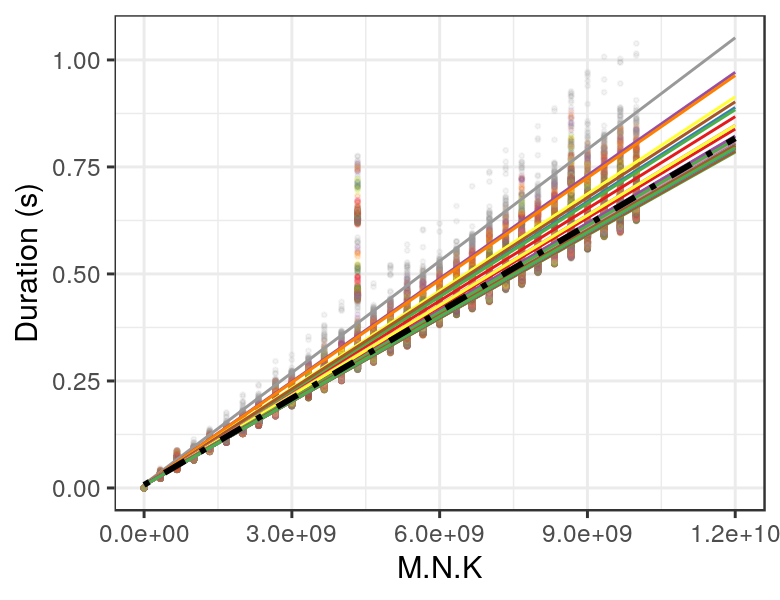
\includegraphics[height=.25\textheight]{img/prediction/modeling/kernels/dgemm_heterogeneity_calib.png}}
                \subfigure[\dgemm
                model\label{fig:dgemm_poly}]{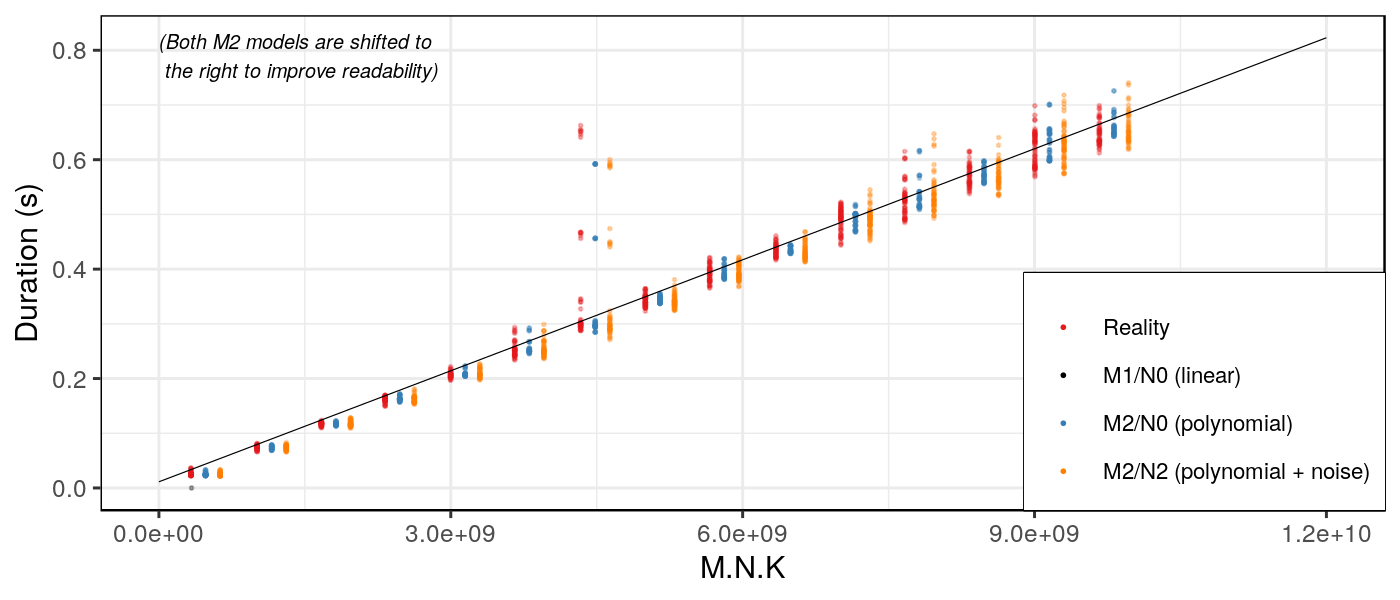
\includegraphics[height=.25\textheight]{img/prediction/modeling/kernels/dgemm_model_calib.png}}
                \caption{Illustrating the realism of modeling for \dgemm function}
                \label{fig:blas_var}
            \end{figure}

            HPL spends the most time in the \dgemm kernel, it is therefore of extreme importance to model this
            function very faithfully.  We  evaluated the previous modeling alternatives:
            \model{\{1,2\}}\noise{\{0,1,2\}} and \model[H]{\{1,2\}}\noise[H]{\{0,1,2\}}.  The \modelp{} and \noisep{}
            families were not investigated as nothing in our observations called for such complexity on classical
            multi-core machines.  Figure\ref{fig:blas_var} illustrates various models and their respective quality for
            the \dgemm function. In these figures, the performance of \dgemm is evaluated by calling
            \dgemm with randomized sizes over all the cores of each node (to reproduce experimental conditions
            similar to the one of HPL). The first observation (Figure\ref{fig:dgemm_het}) is that a few nodes exhibit
            quite a different behavior (each color and each regression line under model \model[H]{1} corresponds to a
            different cpu, whereas the black dotted line corresponds to model \model{1} over all the nodes). These nodes
            will systematically be slightly slower than other nodes and accounting for this spatial heterogeneity is
            likely to be rather important for HPL.  Second, we took care of covering a wide variety of combinations for
            \(M\), \(N\), and \(K\) and it can be observed that \(M.N.K\) is not sufficient to describe correctly the
            performance of \dgemm. Indeed, for \(M.N.K \approx \num{4.5E9}\) some duration are systematically
            higher regardless of the node. This happens for some particular (e.g., tall and skinny) matrix geometries,
            which strongly suggests using the full polynomial model. Figure\ref{fig:dgemm_poly} depicts the performance
            (red dots) of a given node as well as the prediction using a simple linear model (\model[H]{1}, black line),
            a full polynomial model (\model[H]{2}, blue dots) and a full polynomial model with heteroscedastic noise
            (\model[H]{2}\noise[H]{2}, orange dots). A close inspection reveals that all experimental variability is
            actually very well explained by both the polynomial model (better fit for particular parameter combinations)
            and some temporal variability.

            \begin{figure}[ht]
                \centering
                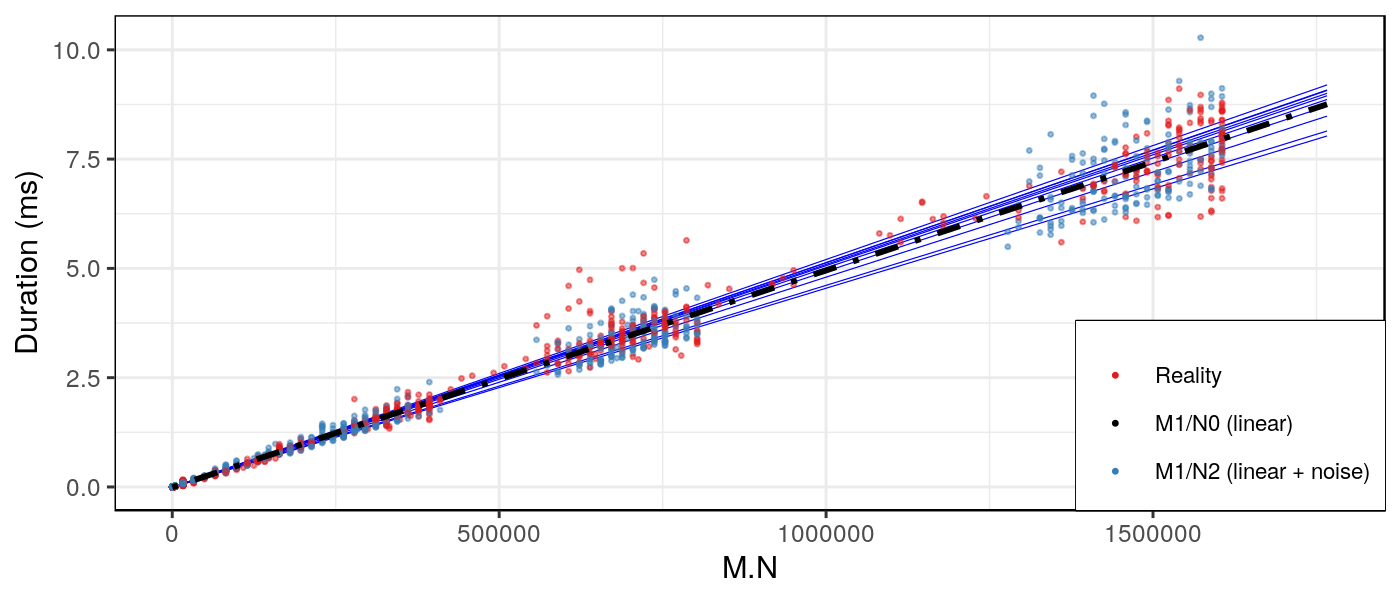
\includegraphics[height=.25\textheight]{img/prediction/modeling/kernels/dlatcpy_model.png}
                \caption{Illustrating the realism of modeling for \texttt{HPL\_dlatcpy} function}
                \label{fig:HPL_var}
            \end{figure}

            Four other BLAS kernels and a few other very small HPL compute kernels (often related to memory management)
            are deeply intertwined with collective operations to allow HPL to be as efficient as possible. Although the
            total duration of these kernels is extremely small compared to the total execution time, they may perturb
            collective communication by introducing late sends and receives. The behavior of one of these kernels is
            illustrated in Figure\ref{fig:HPL_var}. This kind of data can only be obtained by running HPL for a small
            input matrix over each node individually. Again, for all these kernels a single parameter combination
            explains most of the performance and there is some variability from one node to another (one blue regression
            line per CPU) but it remains quite limited (black dotted line for the platform as a whole), especially since
            these kernels are very short and infrequently called compared to \dgemm. Finally, since variability
            significantly increases with the value of the input parameters, a \noise{2} model is clearly required. The
            blue dots in Figure\ref{fig:HPL_var} represent the outcome of a \model{1}\noise{2} model and are hardly
            distinguishable from the real behavior. Similar results can be obtained with this category of model for all
            other kernels.

        \subsection{Bayesian modeling and generative models}%
        \label{sub:dgemm_model:generative_models}

            %% TODO
            %% - Présenter la structure du modèle et la justifier
            %% - Commencer par la régression linéaire + la méthode des moments, STAN
            %%   n'était pas nécessaire pour le papier JPDC.
            %% - Avec Stan pour génerer de nouvelles instances (cf. début de la
            %%   section whatif du JPDC). Stan est overkill et un peu lent finalement
            %%   mais ça pourrait être utile avec un modèle plus complexe (mixture)
            %%   et des données différentes.
            %%   - Note: pourquoi ne pas donner les données brutes à STAN (trop lent
            %%     car trop de données, et convergence super difficile à moins de
            %%     mettre un modèle super sioux).
            In Chapter~\ref{chapter:prediction:validation}, we will show that the model \model[H]{2}\noise[H]{2} is
            required for the \dgemm kernel to make reliable performance predictions for HPL. We recall here the meaning
            of this notation:
            \begin{equation}
                \label{eq:dgemm.complex}
                \begin{split}
                    \text{For each processor $p$, } \textsf{dgemm}_{p}(M, N, K) \sim \mathcal{H}(\mu_{p}, \sigma_{p})\\
                    \begin{cases}
                        \mu_p &= \alpha_pMNK + \beta_pMN + \gamma_pMK + \delta_pNK + \epsilon_p\\
                        \sigma_p &= \omega_pMNK + \psi_pMN + \phi_pMK + \tau_pNK + \rho_p
                    \end{cases},
                \end{split}
            \end{equation}
            where \(\mathcal{H}(\mu, \sigma)\) denotes a random variable following a half-normal distribution with
            parameters \(\mu,\sigma\) accounting for the expectation and the standard deviation. The dependency on \(p\)
            allows to account for platform heterogeneity (since \(\alpha_p,\beta_p, \dots,\rho_p\) can be specific to
            each node), \ie the aforementioned spatial variability. The \(\sigma_p\) parameter allows to account for
            (short-term) temporal variability, \ie to model the fact that the duration of two successive calls to \dgemm
            with the same parameters \(M, N, K\) are never identical.

            As we will show, the performance of nodes exhibits several kinds of variability: i) a spatial variability
            (between nodes) ii) a ``short-term'' temporal variability (the one experienced within an HPL run) but also
            iii) a ``long term'' temporal variability (from a day to another). As illustrated in
            Chapter~\ref{chapter:prediction:validation}, accounting for the first two kinds of variability is essential
            but during our investigation of the simulation validity, which spanned over several months, we also had to
            deal with the fact that the node performance from a day to another could significantly vary, thereby making
            our comparisons between a real experiment and the simulation driven by model obtained with past measurements
            sometimes irrelevant.

            This section explains how all sources of variability can be accounted for in a single unified model. This
            will mainly be used in Chapter~\ref{chapter:prediction:sensibility}. From our observations, we assume that
            on a given node \(p\) and a given day \(d\), the duration of the \dgemm kernel can be modeled as follows:
            \begin{equation}
                \label{eq:dgemm.basic}
                \forall M,N,K, \textsf{dgemm}_{p,d}(M, N, K) \sim \mathcal{H}(\alpha_{p,d}MNK + \beta_{p,d}, \,\, \gamma_{p,d}MNK)\\
            \end{equation}
            Compared to the model~\eqref{eq:dgemm.complex}, this model includes the daily variability but drops the
            complexity of a full-fledged polynomial. Such complexity may be important whenever trying to model a
            particular platform. However, when performing sensibility analysis, a simpler model is preferred, especially
            as not all terms of the polynomial may be statistically significant. In this model, the short-term temporal
            variability stems from the \(\gamma_{p,d}\) term while the average performance of the node stems from the
            \(\alpha_{p,d}\) and \(\beta_{p,d}\) terms, which we gather in a single 3-dimensional vector
            \begin{equation}
              \mu_{p,d}=(\alpha_{p,d},\beta_{p,d},\gamma_{p,d}).
            \end{equation}
            Now, since every machine is unique it is natural to assume that for each machine:
            \begin{equation}
                \label{eq:dgemm.temporal}
                \forall d, \mu_{p,d} \sim \mathcal{N}(\mu_{p},\Sigma_T)
            \end{equation}
            In this model, \(\mu_{p}\) accounts for the average performance of the machine \(p\), while \(\Sigma_T\)
            accounts for its day-to-day variability. From our observation we had no particular reason to assume that
            this variability was different from a machine to another, hence, \(\Sigma_T\) is not indexed by \(p\) but
            global to all machines. However, the parameters \(\alpha_{p,d},\beta_{p,d},\gamma_{p,d}\) are generally
            correlated to each others, hence \(\Sigma_T\) is full covariance matrix to account for interactions.  The
            choice of a Normal distribution is natural since it is the simpler distribution that accounts for a specific
            mean and variance, but we will discuss its relevance later in this section.

            Finally, we need to account for the spatial variability, which we propose to model as follows:
            \begin{equation}
                \label{eq:dgemm.spatial}
                \forall p, \mu_{p} \sim \mathcal{N}(\mu,\Sigma_S)
            \end{equation}
            Again, in such a model \(\mu\) accounts for the machines' average performance while \(\Sigma_S\) accounts
            for the (weak) heterogeneity. This hierarchical model is depicted in Figure~\ref{fig:model:generative}.
            \begin{figure}[pt]
                \centering
                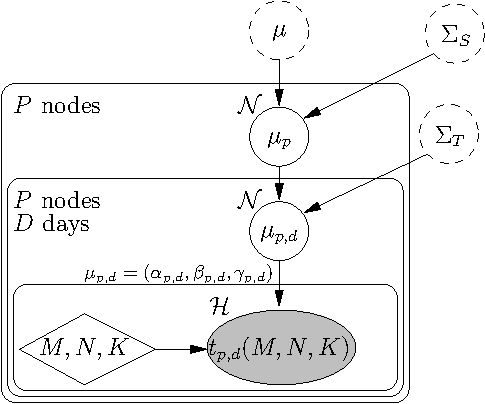
\includegraphics{img/prediction/modeling/kernels//generative_model.pdf}

                \caption{Generative model of kernel duration accounting for the
                  spatial ($\Sigma_S$), long-term ($\Sigma_T$) and short-term variability ($\gamma_{p,d}$). The shaded node
                  represents observed variables and diamond node represents
                  deterministic variables, while non-shaded nodes represent latent
                  variables. The solid node is the variable which is estimated
                  when conducting (in)validation studies while the dashed ones are
                  useful when conducting sensibility analysis and extrapolating to
                  an hypothetical cluster.}
                \label{fig:model:generative}
            \end{figure}

            The relevance of model~\eqref{eq:dgemm.basic} will be discussed in
            Chapter~\ref{chapter:prediction:validation}, but the relevance of models~\eqref{eq:dgemm.temporal}
            and~\eqref{eq:dgemm.spatial} requires some attention.
            Figure\ref{fig:whatif_calibration} represent the empirical distribution of \(\mu_{p,d} =
            (\alpha_{p,d},\beta_{p,d},\gamma_{p,d})\) (the result of the linear regression) for the 32 nodes of the Dahu
            cluster on 40 different days from November 2019 to February 2020. The distribution for each node appears
            approximately normal and passed a Shapiro-Wilk normality test. Although the distribution of the
            \(\beta_{p,d}\) appears slightly skewed toward larger values and one of the nodes (the one with the larger
            \(\alpha_{p,d}\)) stands out, there is no good reason for using a more complex distribution than a Gaussian
            one. Although the correlation between \(\alpha\), \(\beta\), and \(\gamma\) is very weak, it appeared to be
            statistically significant (most ellipses are slightly tilted toward North-East), hence a full variance
            matrix is needed (at least for \(\Sigma_T\)).

            \begin{figure}[pt]
                \centering
                \subfigure[Distribution of $\alpha$, $\beta$, and $\gamma$ (observations on $2\times32$ CPUs from
                    November 2019 to February 2020).  \label{fig:whatif_calibration}]{
                    \raisebox{2em}{\rotatebox{90}{\fbox{\vphantom{y}Real data}}}~%
                    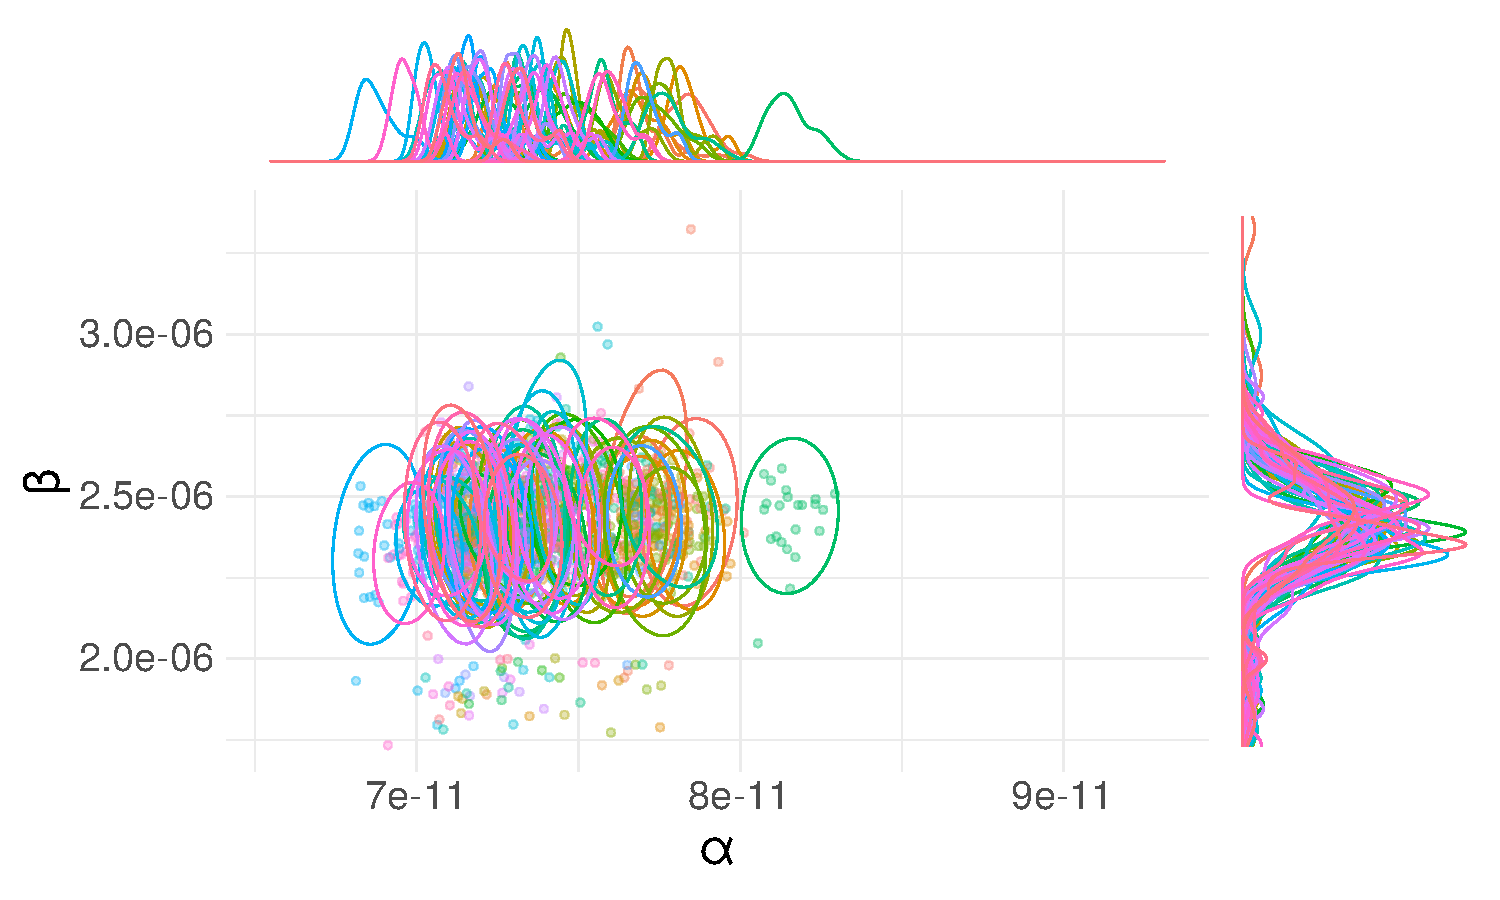
\includegraphics[width=.48\linewidth]{img/prediction/modeling/kernels/whatif_calibration_1.pdf}%
                    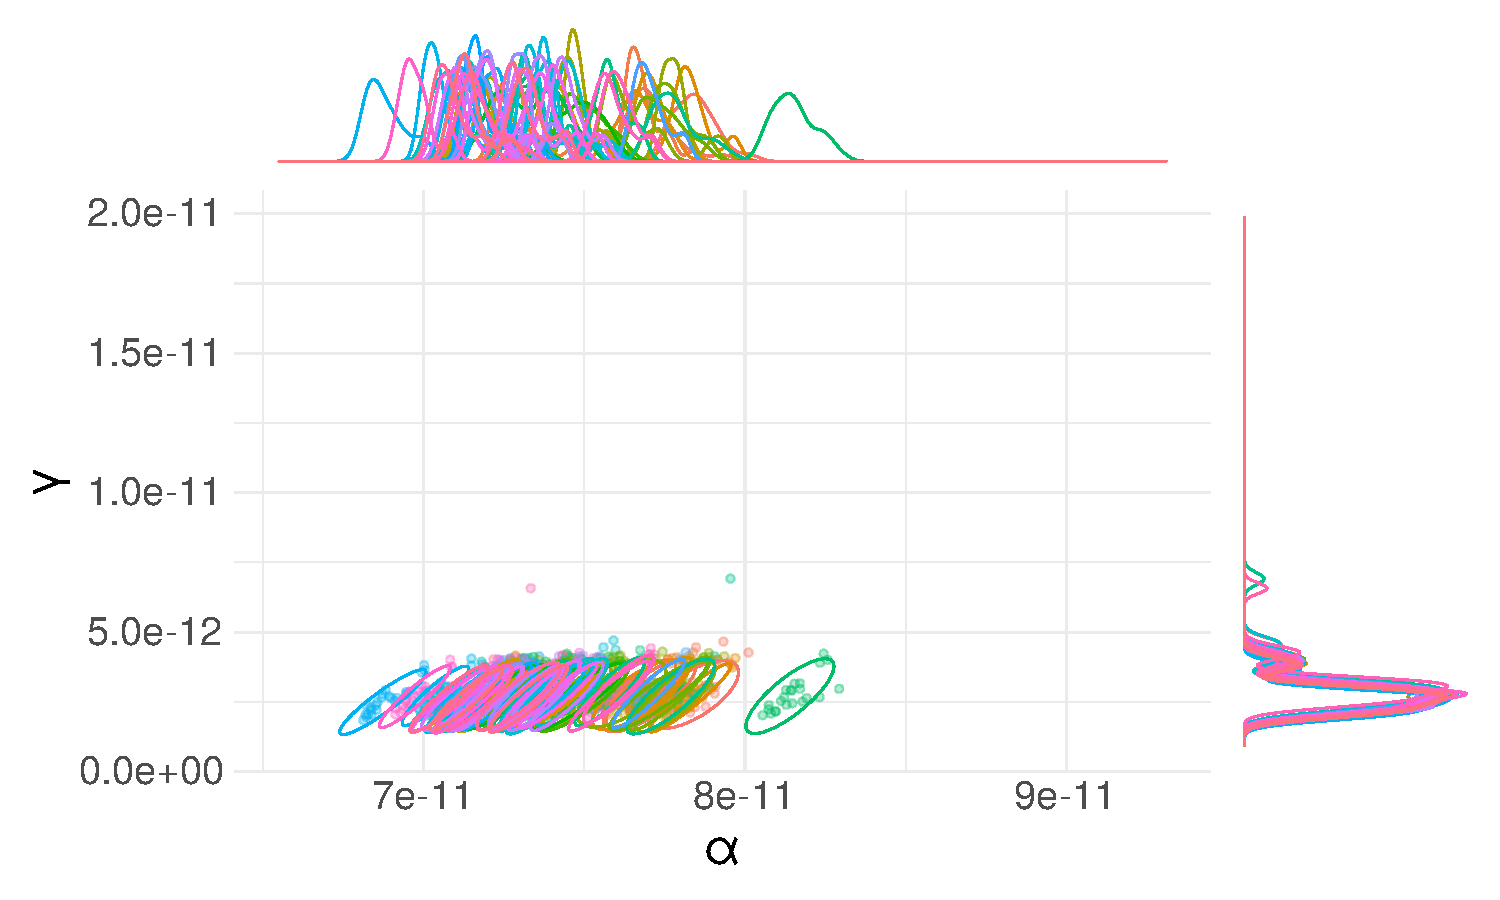
\includegraphics[width=.48\linewidth]{img/prediction/modeling/kernels/whatif_calibration_2.pdf}
                }

                \subfigure[ Distribution of $\alpha$, $\beta$, and $\gamma$ (synthetic data for 16 CPUs).
                    \label{fig:whatif_model}]{
                    \raisebox{1em}{\rotatebox{90}{\fbox{Synthetic data}}}~%
                    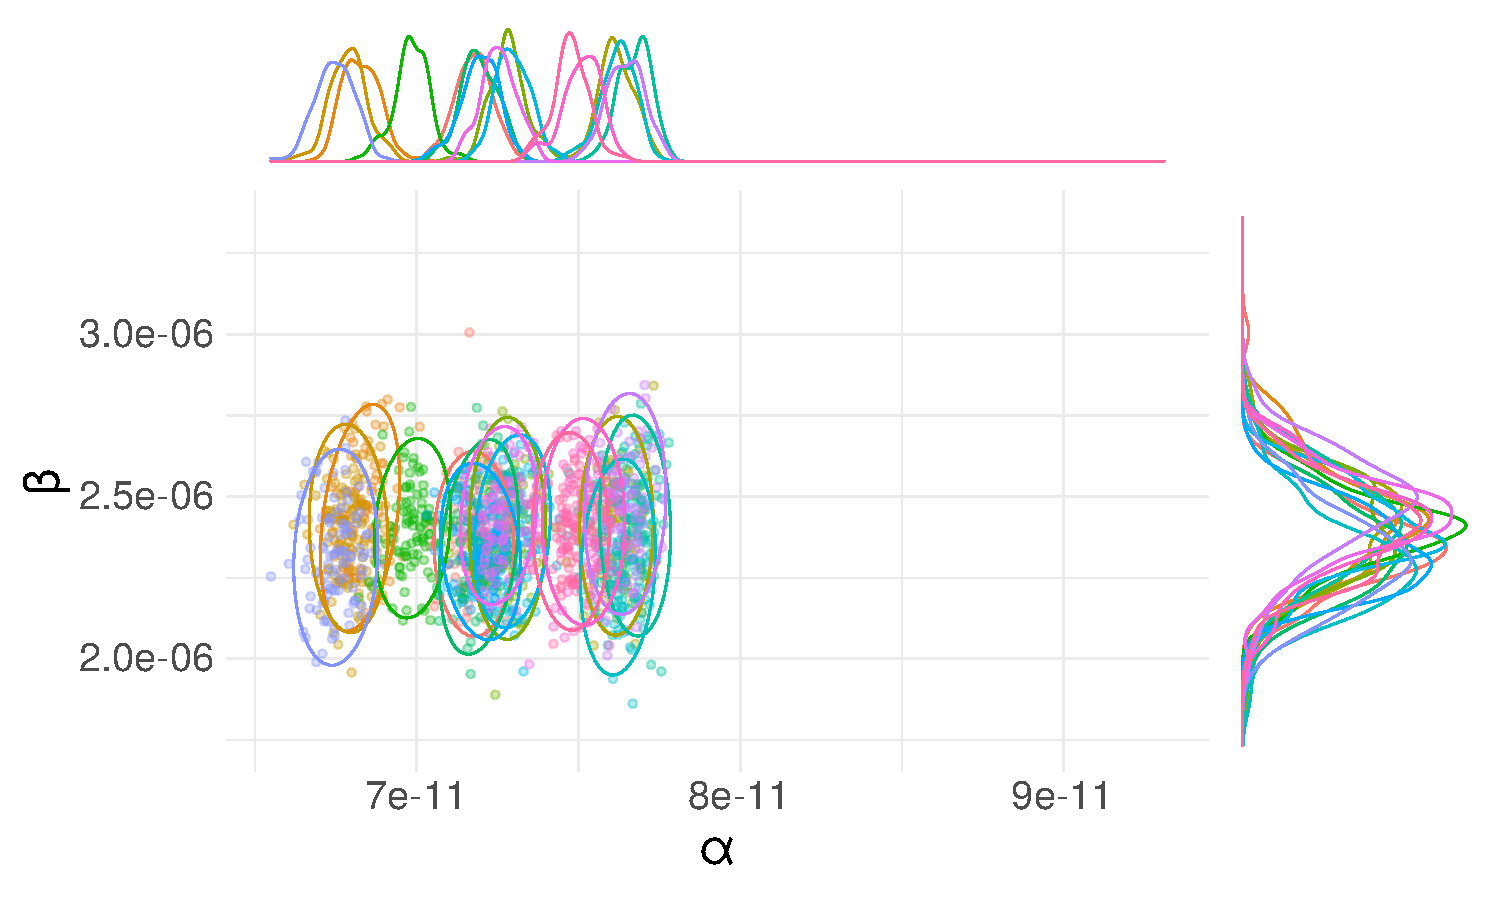
\includegraphics[width=.48\linewidth]{img/prediction/modeling/kernels/whatif_model_1.pdf}%
                    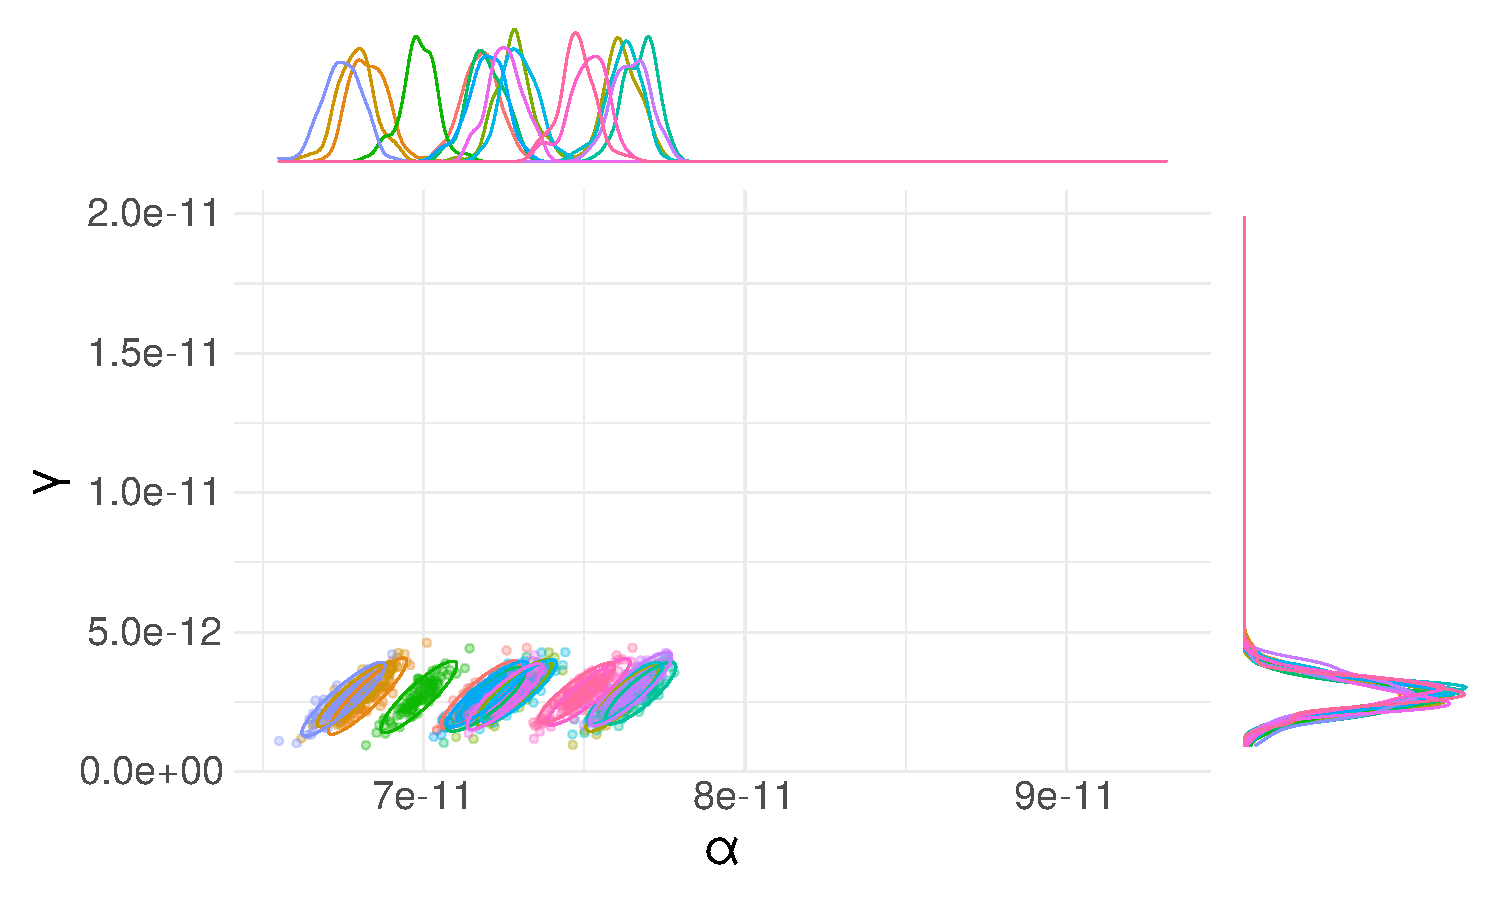
\includegraphics[width=.48\linewidth]{img/prediction/modeling/kernels/whatif_model_2.pdf}
                }
                \caption{Distribution of the regression parameters for around 20 \dgemm calibrations made on
                each of the 32 nodes. Each color/ellipse corresponds to a different CPU.}
                \label{fig:whatif}
                \subfigure[Distribution of $\alpha$, $\beta$, and $\gamma$ (observations on $2\times32$ CPUs
                    from October to November 2019). \label{fig:whatif_slow_calibration}]{
                    \centering
                    \raisebox{2em}{\rotatebox{90}{\fbox{\vphantom{y}Real data}}}~%
                    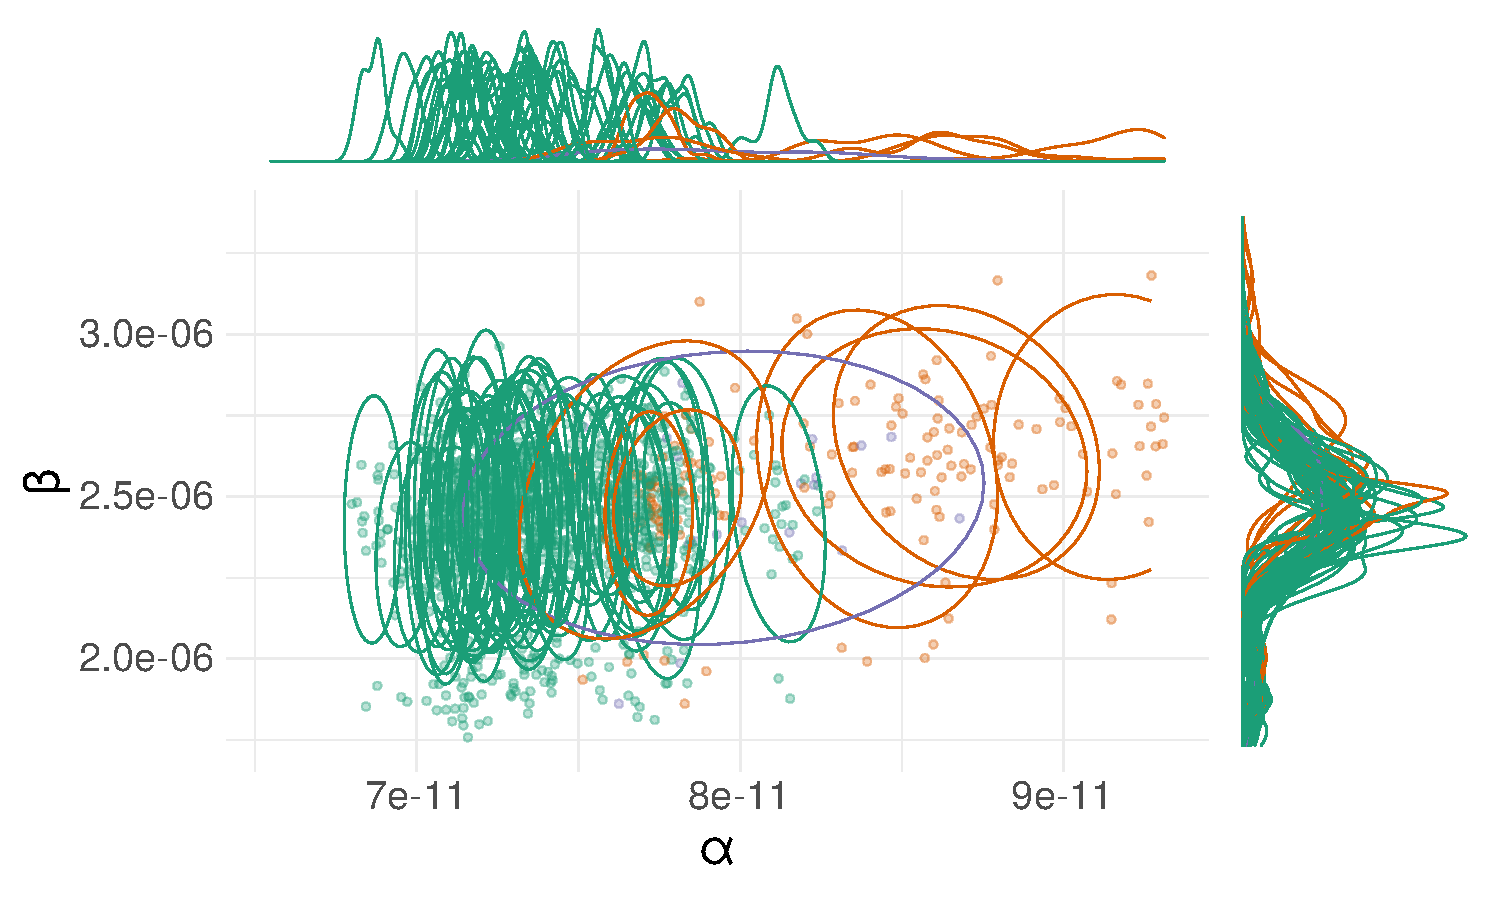
\includegraphics[width=.48\linewidth]{img/prediction/modeling/kernels/whatif_calibration_slownodes_1.pdf}%
                    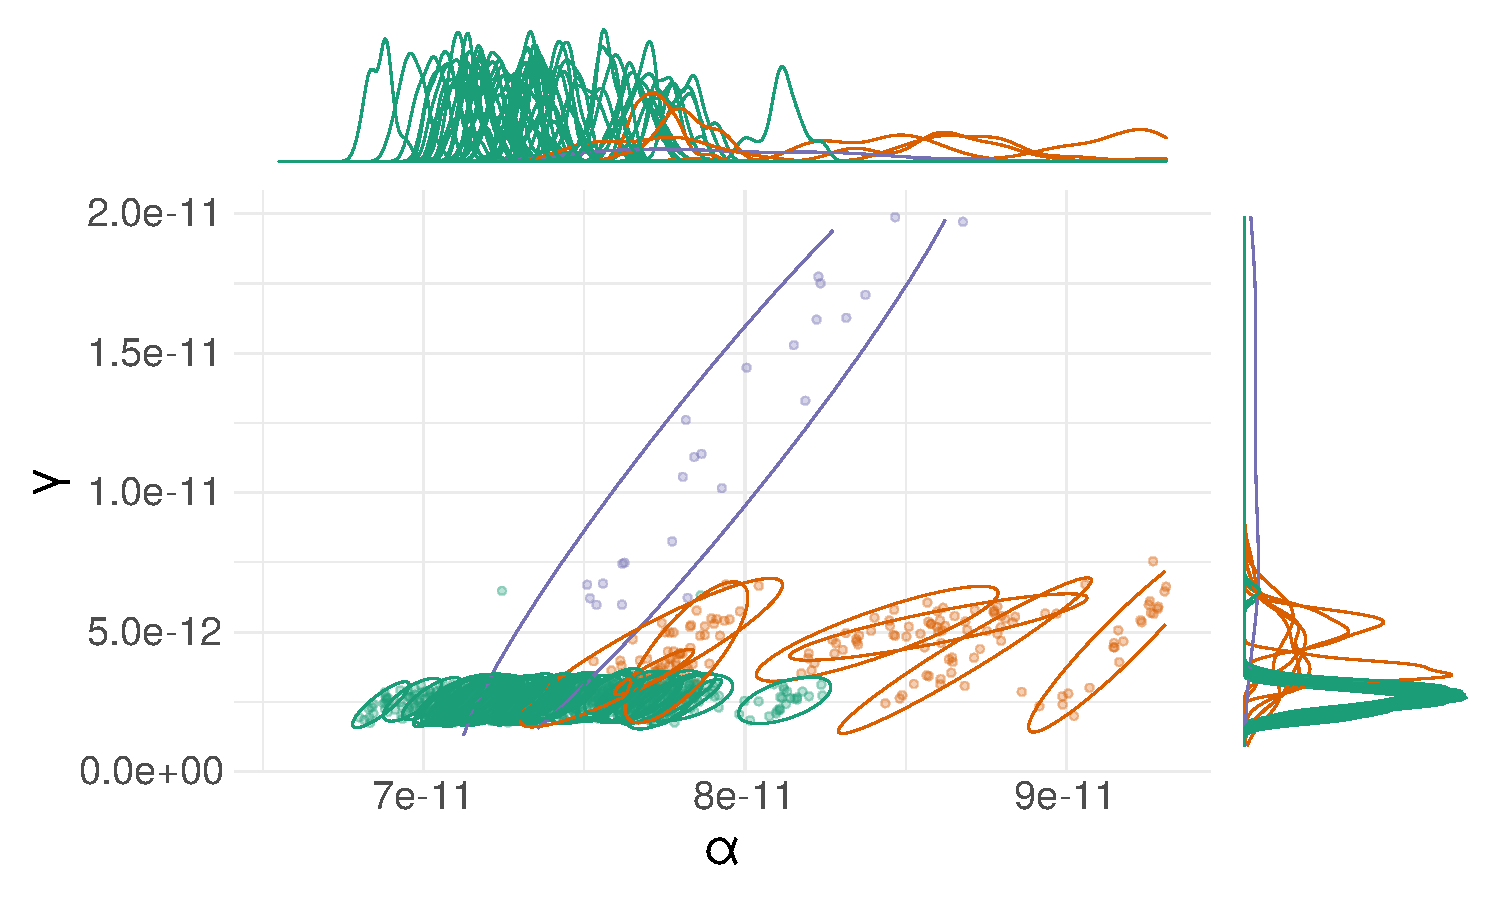
\includegraphics[width=.48\linewidth]{img/prediction/modeling/kernels/whatif_calibration_slownodes_2.pdf}
                }

                \subfigure[Distribution of $\alpha$, $\beta$, and $\gamma$ (synthetic data for 16 CPUs).
                    \label{fig:whatif_slow_model}]{
                    \raisebox{1em}{\rotatebox{90}{\fbox{Synthetic data}}}~%
                    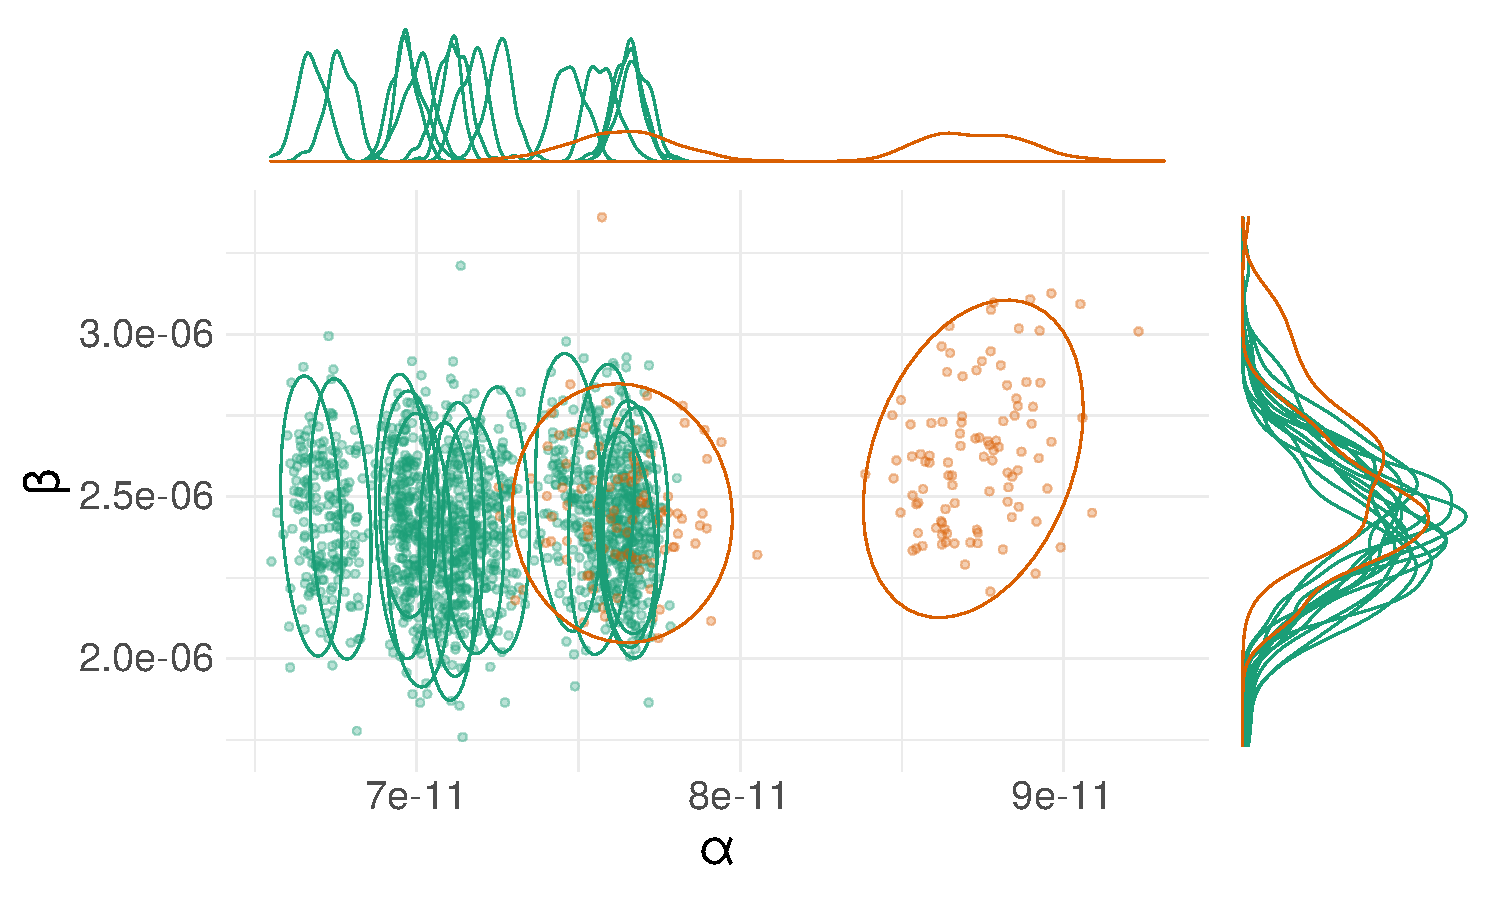
\includegraphics[width=.48\linewidth]{img/prediction/modeling/kernels/whatif_model_slow_1.pdf}%
                    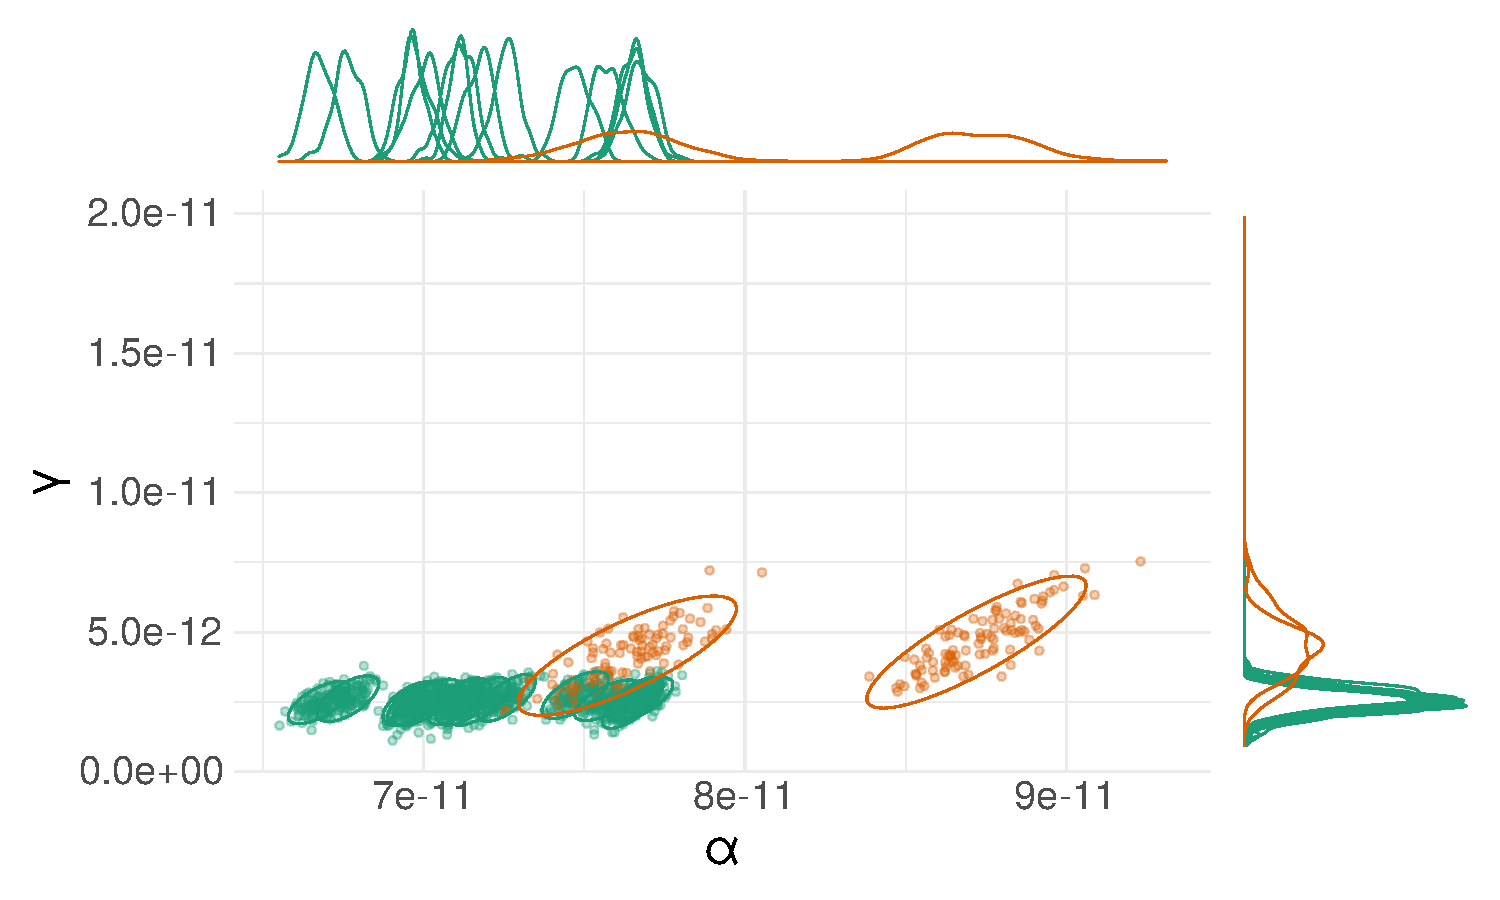
\includegraphics[width=.48\linewidth]{img/prediction/modeling/kernels/whatif_model_slow_2.pdf}
                }
                \caption{Distribution of the regression parameters for around 20
                    \dgemm calibrations made on each of the 32 nodes. 4 of
                    these nodes had a cooling problem, leading to longer and more
                    variable durations. Each
                    color/ellipse corresponds to a different group of CPUs.}
                \label{fig:whatif_slow}
            \end{figure}

            It is thus easy to estimate \(\mu_{p}\) and \(\Sigma_T\) by averaging over the \(\mu_{p,d}\) of each node,
            and then to estimate \(\mu\) and \(\Sigma_S\) by averaging over all the nodes. This moment-matching method
            is simple and provides very good estimates for \(\mu\), \(\Sigma_T\), and \(\Sigma_S\) because we have
            enough measurements at our disposal and because it is particularly suited to the Gaussian modeling
            assumption. Should more complex models (e.g., a mixture to account for ``outlier'' nodes or a SkewNormal
            distribution to account for the distribution's skewness) be used, a general Bayesian sampling framework like
            STAN\cite{stan} would be more adapted. Such frameworks allow to easily specify hierarchical generative
            models like the one presented in Figure~\ref{fig:model:generative} and to draw samples from the posterior
            distribution of \(\mu\), \(\Sigma_T\), and \(\Sigma_S\), which can be used to generate realistic
            \(\mu_{p,d}\) values for a new hypothetical cluster easily.

            Such a process is depicted in Figure~\ref{fig:whatif_model} where hypothetical regression parameters for 16
            nodes have been generated. Comparing such synthetic data with the original samples from
            Figures~\ref{fig:whatif_calibration} allows us to evaluate the model's potential weaknesses. Although the
            orders of magnitude of all parameters and the ellipses are excellent, a few subtle differences are visible.
            First, the variability of \(\alpha_{p}\) seems a bit overestimated (the spread along the x-axis is larger).
            This can be explained by the fact that one of the nodes seemed to be significantly slower (with much larger
            \(\alpha_{p}\)), which artificially increased the spatial variability. Second, as expected from a Gaussian
            model, the distributions of the \(\beta_{p,d}\) are symmetrical whereas there was a slight negative skew in
            the original samples but this should be of little significance for our study. The distributions of the
            \(\gamma_{p,d}\) however are particularly realistic.

            We also illustrate the generality of this model with the data from Figure~\ref{fig:whatif_slow_calibration}.
            These measurements were obtained from October to November 2019 where the cluster was less stable and where
            some nodes particularly misbehaved. Three nodes (in orange, hence a total of 6 CPUs) are distinguished from
            the 28 others (in green) and have lower performance (higher values for \(\alpha\), \(\beta\), and
            \(\gamma\)) and one node (in blue) is particularly unstable. Although this last node may be considered too
            abnormal to represent anything, it would be reasonable to assume that a larger cluster would present at
            least the two kinds of behaviors (green for stable nodes, and orange for slower nodes). The higher layer of
            the model in Figure~\ref{fig:model:generative} should then be replaced by a mixture of normal distributions
            (whose weights would then be sampled from a Dirichlet distribution). Again, hypothetical regression
            parameters for 16 CPUs have been generated with such a process on Figure~\ref{fig:whatif_slow_model} are
            very similar, although different, to the original measurements.

            Overall this model is therefore of excellent quality and can be used to generate large configurations very
            easily and evaluate the influence of different kinds of variability on the performance of HPL.

        \subsection{Conclusion}%
            %% TODO
            %% - Limitation: distinction niveaux de caches, ou bien comportement
            %%   spécifique de la MKL sur KNL. Du piece-wise serait probablement
            %%   bienvenu. Attention aux tailles spécifiques.
            We have described in Section~\ref{sub:dgemm_model:different_models} different models with various levels of
            complexity, from the most basic linear, homogeneous and deterministic model to more elaborated ones with
            heterogeneity and random noise. The objective of Chapter~\ref{chapter:prediction:validation} will be to
            discuss the required level of complexity and (in)validate the quality of these models for faithful
            performance predictions of HPL.

            Then in Section~\ref{sub:dgemm_model:generative_models} we have presented a method for generating new model
            instances based on observed data. This allows to \emph{extrapolate} a given cluster to a larger one or even
            to modify some characteristics of the model such as the temporal or spatial variability. This will be used
            in Chapter~\ref{chapter:prediction:sensibility} for sensibility analysis.

    \section{Modeling the network}
    \label{sec:network_model}

        \subsection{Modelisation in Simgrid}%

            %% TODO
            %% 1. fluide, contention, expérience de saturation des switchs
            %% 2. piecewise, semantic breaks, breaks "multiplicatifs", donc DoE en
            %%    exp(unif) et régression linéaire à la main.
            %% Reprendre de "vieilles figures" pour montrer que c'était fait mais
            %% c'était très manuel. Tentatives d'utilisation de régression linéaire
            %% segmentée mais rien de concluant/fonctionnel jusqu'ici.
            %%
            %% Mentionner le fait qu'on pourrait faire l'analyse et la mesure en même
            %% temps mais que le papier qui faisait ça est assez "naïf" en terme
            %% d'analyse (avec des seuils arbitraires).
            %%
            %% À quoi ressemblent les données brutes avec les breaks et les
            %% mixtures. Pas de structure apparente dans les moment où les mixtures
            %% sont utilisées.
            %%
            %% Mini-conclusion: le modèle de nos rêves (breakpoints + mixture). Bien
            %% plus compliqué que pour le CPU car paramètres à trouver et bruit
            %% vraiment compliqué. Il existe des choses pour les mixtures seules,
            %% sous certaines hypothèses (homoscedastique). Pour les breakpoints, on
            %% va expliquer dans la suite.

            Prior to this work, the standard way of accounting for protocol changes in SMPI was to estimate breakpoints
            visually and to conduct a linear regression for each range. The expected duration was then used directly in
            the simulation with no particular effort with respect to the temporal variability (\modelp{1}\noise{0}).
            Yet, as illustrated in Figure\ref{fig:nw_var}, the variability of high speed networks is quite particular,
            for some intervals of message sizes the observed durations have several modes. These modes happen
            homogeneously during the calibration experiment, they are not caused by a transient perturbation of the
            system.

            \begin{figure}[ht]
                \vspace{-1em}
                \centering 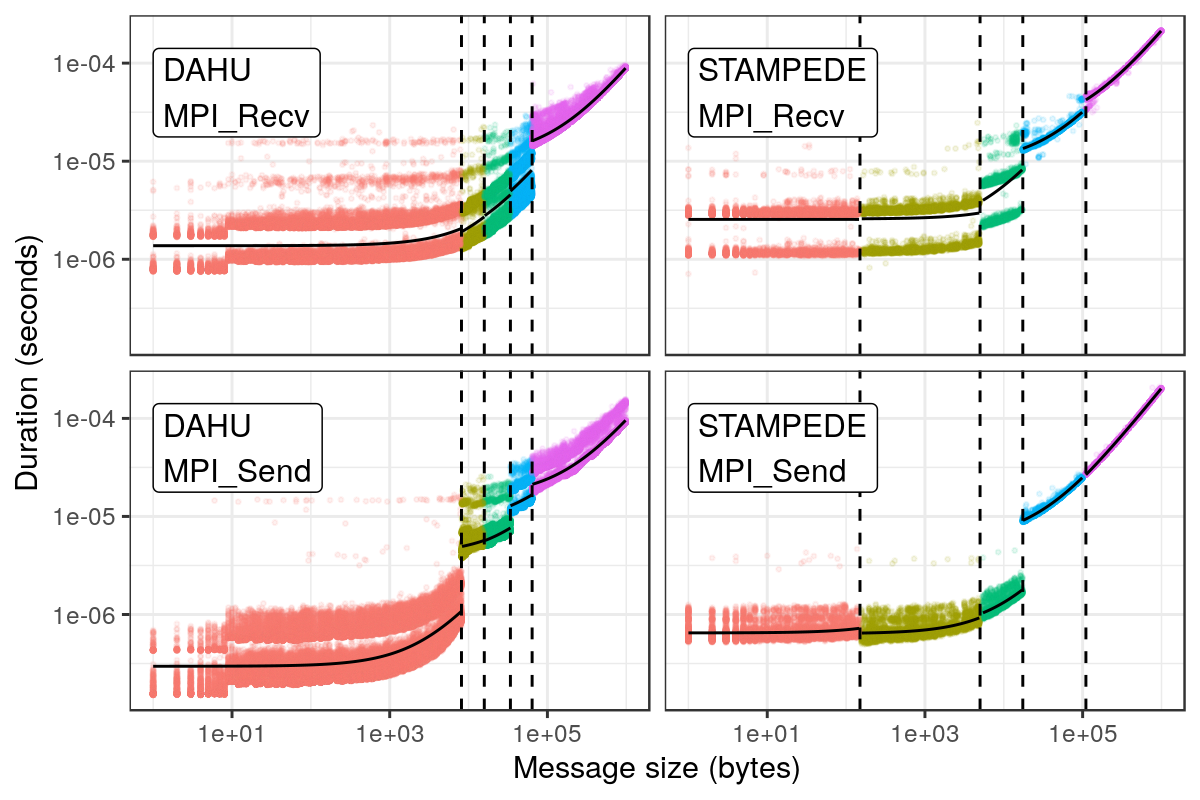
\includegraphics[width=.9\linewidth]{./img/prediction/modeling/network/mpi_calibration.png}
                \caption{Illustrating piecewise linearity and temporal variability of high-speed communications on two
                systems.}
                \label{fig:nw_var}
            \end{figure}

            The ideal model for such observed data would be \modelp{1}\noisep{1}, several intervals of message sizes
            with abrupt breakpoints, and a noise distributed as a Gaussian mixture for each range.  Such temporal
            variability could explain some (overall bad) performance since they generally get amplified by broadcast and
            pipelined communication patterns.

            Automatically computing the best fit for a complex model like the abovementionned one is way more difficult
            than for the \dgemm model proposed in Section~\ref{sec:network_model}. It should be possible to compute it
            in one go with a Bayesian framework like STAN, but it would probably be computationally prohibitive. A more
            realistic solution is to perform two steps: (1) average the durations per message size and find the
            breakpoints using this aggregated data, and (2) on each segment, compute the linear regression with a noise
            mixture.
            \begin{enumerate}
                \item We have tested two different solutions for computing a piecewise linear regression, a Python
                    package named \texttt{datadog-piecewise}~\cite{datadog}, and an R package named
                    \texttt{cubist}~\cite{cubist}.  Although both of them work perfectly on the simplest generated
                    datasets, they did not produce satisfying results with our real data. The likely reason is both the
                    exponential distribution of the predictor variable and the heteroscedasticity of the noise. We made
                    the choice  to implement our own solution, detailed in Section~\ref{sub:pycewise}.
                \item We tested an existing R package named \texttt{flexmix} for computing a linear regression with a
                    Gaussian mixture noise~\cite{flexmix}. It revealed to be fragile, the result being
                    non-deterministic: the number of modes found by the algorithm was not constant. We ended up
                    clustering the data manually with a visual inspection and then computing a simple linear regression
                    for each mode.
            \end{enumerate}

        \subsection{Learning breakpoints}%
        \label{sub:pycewise}

            %% TODO
            %% - Algorithme "haut-niveau" avec les deux phases, top-down & bottom-up.
            %% - Implémentation efficace pour la régression linéaire classique.
            %% - Faiblesse de la recherche automatique de breakpoints sur certains exemples.
            %% - Implémentations alternatives : régression pondérée, régression log (y a-t-il
            %%   un nom officiel pour ce que l'on a fait ?).
            %%   - Maximum Likelihood avec modèle log-normal.
            %%   - Note: si lognormal avec mixtures, pourquoi ne pas donner les
            %%     données brutes à STAN. Convergence déjà super difficile avec
            %%     notre approche adhoc et s'il fallait rajouter un algorithme d'EM
            %%     en plus pour les mixtures et les breakpoints, c'est juste pas
            %%     raisonnable.
            %% - Détailler un peu l'implémentation, ces méthodes sont moins rapides
            %%   que la première version.
            %% - Comparaison des trois méthodes sur tous les exemples que j'ai.
            In this section, we present our solution for automatically computing a piecewise linear regression. This has
            been implemented as a Python package named
            \texttt{pycewise}\footnote{\url{https://github.com/Ezibenroc/pycewise}}.

            \subsubsection{Model}%

                We define here the base asumptions and notations for our optimization problem. The predictor variables
                (\eg the message size) will be noted \(X\), the response variables (\eg the communication duration) will
                be noted \(Y\). We will note \(\ell\) the list of tuples \((X,Y)\). We suppose there are \(N\) different
                unknown breakpoints \(B_1 < \dots < B_N\), where \(N\) itself is also unknown. For convenience, we will
                note \(B_0=-\infty\) and \(B_{N+1} = +\infty\).  Then, there are \(N+1\) tuples \((\alpha_i, \beta_i,
                \gamma_i, \delta_i)\) such that:
                \begin{align}\label{eqn:prediction:pycewise_model}
                    Y \sim \alpha_i X + \beta_i + \mathcal{N}\left(0, \gamma_i X + \delta_i\right)
                        && \text{ if } B_i \leq X < B_{i+1}
                \end{align}

                Here, \(\gamma_i\) may be null (homoscedastic data) or non-null (heteroscedastic data). This hypothesis
                will be discussed later. Likewise, the distribution of the \(B_i\) will be discussed when comparing
                different solutions, no assumption is made yet.

                A \emph{solution} \(\theta\) to the optimization problem consists in the list of breakpoints \((B_i)\)
                and tuples \((\alpha_i,\beta_i)\). The values \((\gamma_i, \delta_i)\) are not computed here, they could
                be estimated in a second phase. We will write \(f_\theta\) the (deterministic) prediction function
                associated with the solution:
                \begin{align}
                    f_{\theta}(X) = \alpha_i X + \beta_i
                        && \text{ if } B_i \leq X < B_{i+1}
                \end{align}

                Two objective functions are considered:
                \begin{itemize}
                    \item \(\text{RSS}(\ell, \theta) = \sum_{(X,Y)\in\ell} (Y-f_\theta(X))^2\) is the usual residual sum
                        of squares.
                    \item \(\text{BIC}(\ell, \theta) = K\log(S) + S\log(\text{RSS}(\ell, \theta))\) where \(S=|\ell|\)
                        is the number of observations, \(K = 3(N+1)+N = 4N+3\) is the number of parameters in the
                        model. This is the usual bayesian information criterion.
                \end{itemize}

                The goal of the optimization problem is to minimize the BIC. The \(K\log(S)\) term in this function is
                intended to penalize the model size and thus prevent overfitting.

                By an abuse of notation, we will write \(\text{BIC}(\ell)\) the BIC for the observations \(\ell\) with a
                simple linear regression without breakpoint (\ie \(N=0\)). We will write
                \(\text{BIC}(\ell_1\oplus\ell_2)\) the BIC for the observations \(\ell_1 \cup \ell_2\) with a single
                breakpoint between the two lists and a simple linear regression for each list (\ie \(N=1\)).
                The concatenation of lists will be noted \(\ell_1 \bullet \ell_2\), hence
                \(\text{BIC}(\ell_1\bullet\ell_2)\) will denote the BIC of a linear regression without breakpoint
                (\(N=0\)).

            \subsubsection{Main algorithm}%

                The algorithm is made of two steps, it starts by a top-down step where new breakpoints are
                greedily added, it finishes by a bottom-up step where some breakpoints are greedily removed to simpify
                the solution. The first step is inspired by the work of Malerba~\etal~\cite{Malerba_2004}.

                In the top-down step (Algorithm~\ref{algo:pycewise:topdown}), we recursively build a tree, where the inner
                nodes represent a breakpoint and the leaves represent a simple linear regression. The function
                \texttt{topdown} takes as input a list \(\ell\) of tuples \((X,Y)\) sorted by increasing \(X\) and
                returns a list of sublists, each sublist representing an interval for the piecewise regression. On a
                given call, we iterate on the list to test all the \(X\) as a possible breakpoint, we search for the
                \(X\) that minimizes the objective function.  If the objective with the new breakpoint is smaller than
                the objective without breakpoint, then we recursively call the function on the two sub-lists.
                \begin{algorithm}
                    \DontPrintSemicolon
                    \SetKwFunction{Ftopdown}{topdown}
                    \SetKwProg{Fn}{Function}{:}{}
                    \Fn{\Ftopdown{\(\ell\)}}{
                        \(\text{best\_BIC} = +\infty\)\;
                        \ForEach{\((X,Y) \in \ell\)}{
                            split \(\ell\) into \(\ell_1\) and \(\ell_2\) such that
                                \(\forall X'\in\ell_1, X'\leq X\)
                                and \(\forall X'\in\ell_2, X'> X\)\;
                            \(\text{new\_BIC} = \text{BIC}(\ell_1 \oplus \ell_2)\)\;
                            \If{\(\text{new\_BIC} < \text{best\_BIC}\)}{
                                \(\text{best\_BIC} = \text{new\_BIC}\)\;
                                \(\text{best\_solution} = (\ell_1, \ell_2)\)\;
                            }\;
                        }\;
                        \uIf{\(\text{new\_BIC} < \text{BIC}(\ell)\)}{
                            \((\ell_1, \ell_2) = \text{best\_solution}\)\;
                            \(\text{lists}_1\) = \Ftopdown{\(\ell_1\)}\;
                            \(\text{lists}_2\) = \Ftopdown{\(\ell_2\)}\;
                            \KwRet{\(\text{lists}_1 \oplus \text{lists}_2\)}\;
                        }
                        \Else{
                            \KwRet{\(\ell\)}\;
                        }
                    }
                    \caption{Top-down step for computing the piecewise linear regression}
                    \label{algo:pycewise:topdown}
                \end{algorithm}

                In our implementation, each iteration of the \texttt{foreach} loop from
                Algorithm~\ref{algo:pycewise:topdown} is executed in a constant time. This is possible because the list
                \(\ell\) is sorted by increasing \(X\), no copies are made when splitting the list, and both the new linear
                regressions and the new BIC are computed with online algorithms (\ie adding or removing one tuple
                \((X,Y)\) from the sublists \(\ell_1\) and \(\ell_2\) does not require to recompute from scratch the new
                regression coefficients nor the BIC, it is possible to update the values from the previous iterations).
                In the next sections, we changed the objective function and had to drop this quality of doing an
                iteration in constant time, the effect on the computation duration will be discussed.

                In the bottom-up step (Algorithm~\ref{algo:pycewise:bottomup}), adjacent intervals are greedily merged
                (thereby removing breakpoints), starting by fusions that decrease the least the RSS. All the different
                iterations of the loop are kept in memory, the merging operation is carried until there is no breakpoint
                left. In the end, we keep the iteration that minimized the BIC.
                \begin{algorithm}
                    \DontPrintSemicolon
                    \SetKwFunction{Fbottomup}{bottomup}
                    \SetKwProg{Fn}{Function}{:}{}
                    \Fn{\Fbottomup{\(L = (\ell_1,\dots,\ell_{N})\)}}{
                        \(S\) = []\;
                        add \(L\) to \(S\)\;
                        \For{\(i=1\) \KwTo \(N-1\)}{
                            \(\text{best\_diff} = +\infty\)\;
                            \(n = N-i\)\;
                            \For{\(j=1\) \KwTo \(n-1\)}{
                                \(\text{new\_diff} = \text{RSS}(\ell_j \bullet \ell_{j+1}) - \left(\text{RSS}(\ell_j) +
                                    \text{RSS}(\ell_{j+1})\right)\)\;
                                \If{\(\text{new\_diff} < \text{best\_diff}\)}{
                                    \(\text{best\_diff} = \text{new\_diff}\)\;
                                    \(k = j\)\;
                                }\;
                            }\;
                            \(L = (\ell_1,\dots,\ell_{k}\bullet\ell_{k+1},\dots,\ell_n)\)\;
                            add \(L\) to \(S\)\;
                        }\;
                        let \(L \in S\) be the solution with minimal BIC\;
                        \KwRet{\(L\)}\;
                    }
                    \caption{Bottom-up step for computing the piecewise linear regression}
                    \label{algo:pycewise:bottomup}
                \end{algorithm}

                \pagebreak

            \subsubsection{Objective function}%
                The breakpoint learning process relies entirely on the objective function we defined, based on the
                residual sum of squares (RSS) and its BIC counterpart that penalizes the model size:
                \begin{equation}
                    \text{RSS}(\ell, \theta) = \sum_{(X,Y)\in\ell} (Y-f_\theta(X))^2
                \end{equation}
                The algorithm is an heuristic to minimize the BIC, but the parameters of the linear regressions are
                also the optimal estimators for this objective function.

                In the case of heteroscedastic data, the noise is by definition not constant, it grows linearly with the
                predictor variable. In this case, the RSS is not the best choice, as it does not penalize errors
                relatively to the predictor variable. It will give much more weight to the larger noise observed for
                larger predictor variables, hence a bias towards those large values.

                A classical solution for this problem is the use of weighted least square (WLS) instead of the ordinary
                least square (OLS). A weight function \(w\) gives a different weight for each predictor variable. We
                define the new objective function as such:
                \begin{equation}
                    \text{RSS}_\text{weight}(\ell,\theta) = \sum_{(X,Y)\in\ell} (w(X)(Y - f_\theta(X)))^2
                \end{equation}
                The \(\text{BIC}_\text{weighted}\) value is defined like the BIC, replacing the RSS value by
                \(\text{RSS}_\text{weight}\).
                In our case, we used \(w(X) = 1/X\), a classical choice for linear regressions in the presence of
                heteroscedasticity.

                As said previously, the optimal values for the regression parameters are not the same with this
                objective function. A closed formula can be found by taking the derivative of the function, very
                similarly to the ordinary least square.
                \begin{equation}
                    \hat\alpha_\text{weight} = \frac{\sum_{(X,Y) \in \ell}
                    w(X)(X-\hat{X}_\text{weight})(Y-\hat{Y}_\text{weight})}
                    {\sum_{(X,Y) \in \ell} w(X)(X-\hat{X}_\text{weight})^2}
                \end{equation}
                \begin{equation}
                    \hat\beta_\text{weight} = \hat{Y}_\text{weight} - \hat{\alpha}_\text{weight}\hat{X}_\text{weight}
                \end{equation}
                Here, \(\hat{X}_\text{weight}\) (resp. \(\hat{Y}_\text{weight}\)) denotes the weighted sample mean of
                the variables \(X\) (resp. \(Y\)), computed as:
                \begin{equation}
                    \hat{X}_\text{weight} = \frac{\sum_{(X,Y)\in\ell}w(X)X}{\sum_{(X,Y)\in\ell}w(X)}
                \end{equation}
                \begin{equation}
                    \hat{Y}_\text{weight} = \frac{\sum_{(X,Y)\in\ell}w(X)Y}{\sum_{(X,Y)\in\ell}w(X)}
                \end{equation}

                An alternative objective function is based on the logarithm of the observations and the predictions:
                \begin{equation}
                    \text{RSS}_{\log}(\ell,\theta) = \sum_{(X,Y)\in\ell} (\log Y - \log f_\theta(X))^2
                \end{equation}
                Likewise, the value \(\text{BIC}_{\log}\) is naturally defined based on \(\text{RSS}_{\log}\). The main
                motivation here is to penalize the prediction error relatively to the predictor variable and not in
                absolute value.

                With such an objective function, there is no closed form for the optimal regression parameters. Instead,
                we implemented a gradient descent algorithm to find the optimum.
                The downside of using a gradient descent is that the whole regression is now significantly slower, the
                extent of this will be discussed later. On the other hand, a nice benefit is the possibility to tune the
                objective function to better suit our needs. For instance, in the case of network calibrations, the
                regression parameters \(\alpha\) and \(\beta\) represent respectively the inverse of the bandwidth and
                the latency, it would make no sense for them to be negative. With the gradient descent approach, the
                search space can easily be restricted to limit the possible solutions to positive values.

            \subsubsection{Comparison of the solutions}%

                We compared different approaches for computing a piecewise linear regression. We used a typical dataset
                for our context that has similar characteristics than the network calibration data (see
                Figure~\ref{fig:nw_var}): the predictor variable is sampled exponentially and the noise is
                heteroscedastic.

                The different approaches are presented in Figure~\ref{fig:prediction:pycewise}. Each row presents one
                solution, the first two rows are Datadog-piecewise~\cite{datadog} and Cubist~\cite{cubist}. The last
                three rows are our proposed implementation with the three discussed objective functions. The black
                points represent the observations, the colored lines represent the linear regressions, while the
                different breakpoints are marked with a dashed vertical line.

                \begin{figure}[htpb]
                    \centering
                    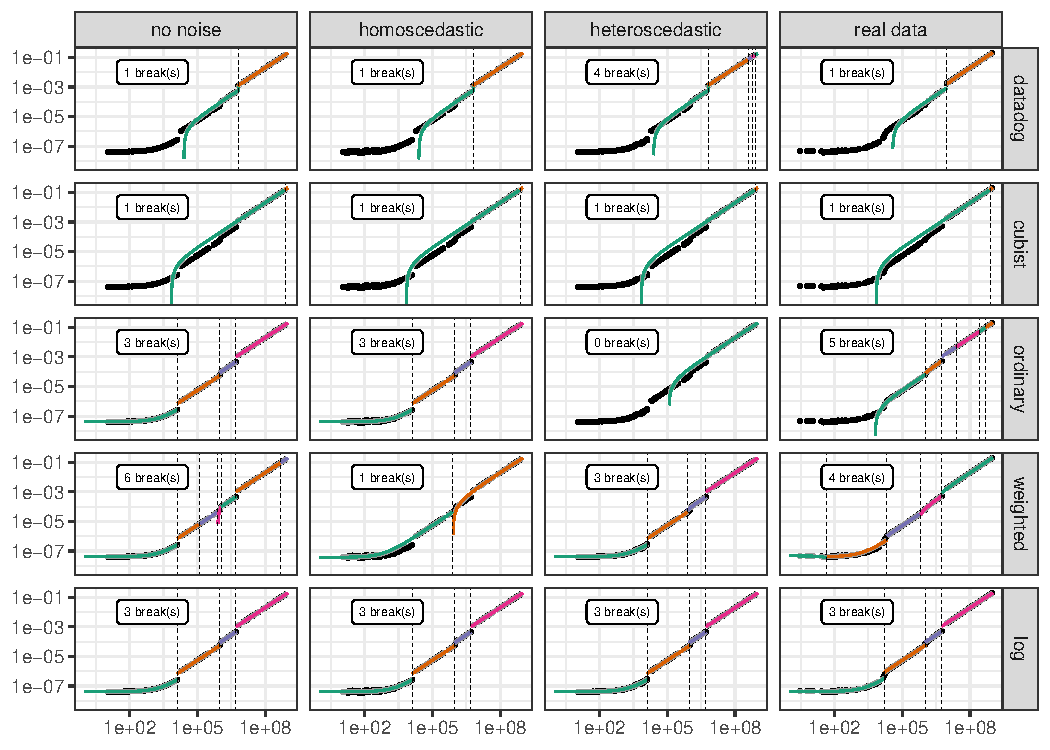
\includegraphics[width=\linewidth]{img/prediction/modeling/network/pycewise.pdf}
                    \caption{Illustrating different piecewise linear regression approaches on different datasets. Only
                    the logarithmic objective function works well for all datasets.}%
                    \label{fig:prediction:pycewise}
                \end{figure}

                Four variations of the dataset are used, one variation per column:
                \begin{itemize}
                    \item The real data comes from a real experiment we performed on a node, these are durations of
                        calls to \texttt{memcpy} function for various buffer sizes. Each point is the average of several
                        measures with a same size, so we can reasonably expect the noise to be normally distributed.
                    \item The three other variations are generated data. We performed a piecewise linear regression on
                        the real data with three manually selected breakpoints, we sampled a new series of predictor
                        variables, then we computed the expected durations. The response variables of the \emph{no
                        noise} dataset are entirely deterministic.
                    \item The \emph{homoscedastic} dataset has been generated by adding a normally distributed noise of
                        mean 0 and standard deviation \Num{5e-9} to the \emph{no noise} dataset.
                    \item The \emph{heteroscedastic} dataset has been generated by adding a normally distributed noise
                        of mean 0 and standard deviation \(\Num{2e-12}\times X\) to the \emph{no noise} dataset, where
                        \(X\) denotes the predictor variable.
                \end{itemize}

                The goal of using generated data was to understand better the limitations of each approach. From
                Figure~\ref{fig:prediction:pycewise}, it is clear that both Datadog-piecewise and Cubist are unfit for
                our needs (first and second rows), as they could not even find the three breakpoints with the generated
                data without noise. The likely reason is the exponential sampling of the predictor variable, the points
                on the left part of the plots would get compressed into a single point if the data was plotted in linear
                scale.

                As expected, the ordinary least square method (third row) works perfectly in the absence of noise or
                with homoscedastic noise, as it finds the three breakpoints. Unfortunately, it fails to find any
                breakpoint with the heteroscedastic noise. With the real data, it finds too many of them for large
                values but misses an obvious breakpoint for smaller values near \Num{1e4}.

                The weighted least square method (fourth row) works as expected with heteroscedastic data, finding the
                three breakpoints. It also performs quite well with the real data, finding three obvious breakpoints,
                but it also detects a spurious one near the smallest values. It also fails spectacularly with the two
                other datasets, missing obvious breakpoints with the homoscedastic data and finding too many with the
                no-noise data.

                In the end, only the logarithmic least square method (last row) works perfectly for all the datasets.

                Another interesting feature of the last method is the positivity constraint. With this approach, it is
                possible to force the two parameters of each linear regression to be positive, as discussed previously.
                The three other methods all have an issue for at least one dataset where the intercept of one regression
                is negative, resulting in negative predictions when the predictor variable is too low. This can be seen
                when the prediction lines falls very sharply on the left. Note that this positivity constraint is only
                due to the gradient descent implementation and not to the objective function, we could very well
                add a similar constraint for the other objective functions if they were also implemented with a gradient
                descent instead of a simple formula.

                The quality of the fit computed by pycewise with the logarithmic objective function is demonstrated in
                Figure~\ref{fig:prediction:pycewise_demo}. We executed our MPI calibration program on four clusters of
                Grid'5000: dahu, gros, paravance and pyxis. For each of them, we measured the duration of individual
                \recv, \send and a whole ping-pong for various message sizes. Once again, we aggregated the data by
                taking the average duration for each message size. In this figure, one piecewise regression is computed
                for each cluster/operation pair.

                \begin{figure}[htpb]
                    \centering
                    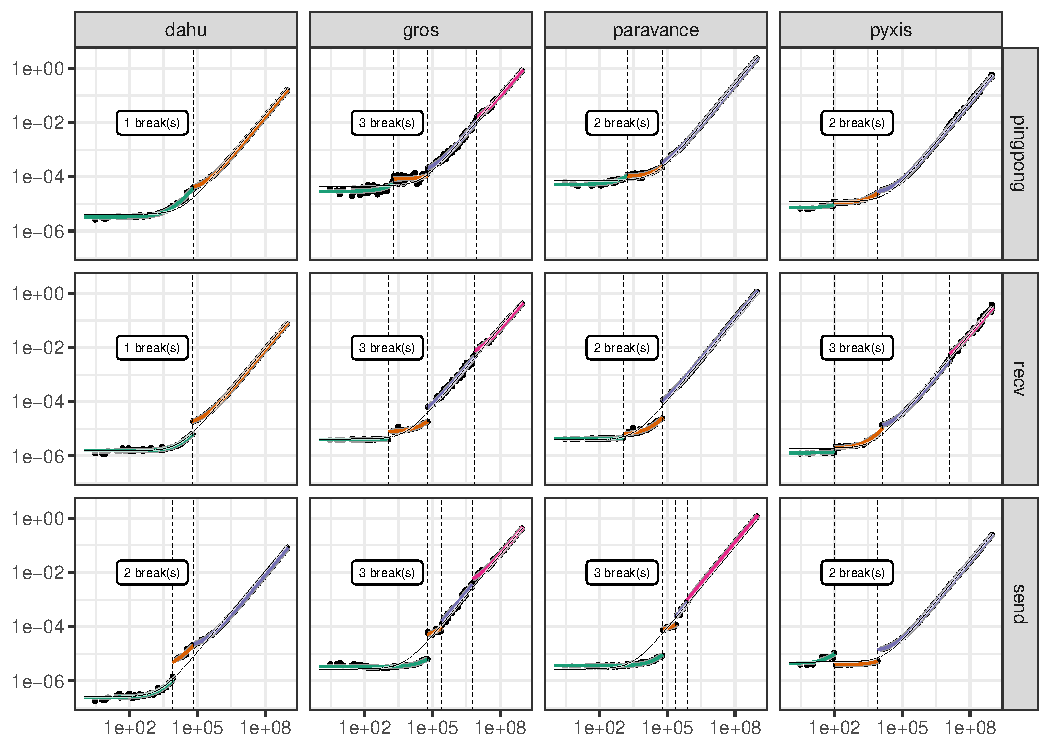
\includegraphics[width=\linewidth]{img/prediction/modeling/network/pycewise_demo.pdf}
                    \caption{With the logarithmic objective function, pycewise finds acceptable fits for the 12 datasets}%
                    \label{fig:prediction:pycewise_demo}
                \end{figure}

                Since this is real experimental data, there is no "ground truth" that could serve as reference for
                evaluating the quality of the fit. Computing the optimal solution which minimizes the objective function
                would be computationally intractable. Therefore, we can only rely on a visual evalution of the
                regression lines to decide if the fits are satisfying. In Figure~\ref{fig:prediction:pycewise_demo}, all
                the obvious breaks have been found and the lines match the points very closely.

                This gradient descent comes with a cost, computing the piecewise linear regression is now significantly
                slower. Figure~\ref{fig:prediction:pycewise_duration} compares the three different objective functions
                from our implementation. The logarithmic least square is one order of magnitude slower than the weighted
                least square, which is itself one order of magnitude slower than the ordinary least square. The nature
                of the noise does not affect the duration, but we expect that a dataset with more breakpoints would lead
                to a larger duration.
                \begin{figure}[htpb]
                    \centering
                    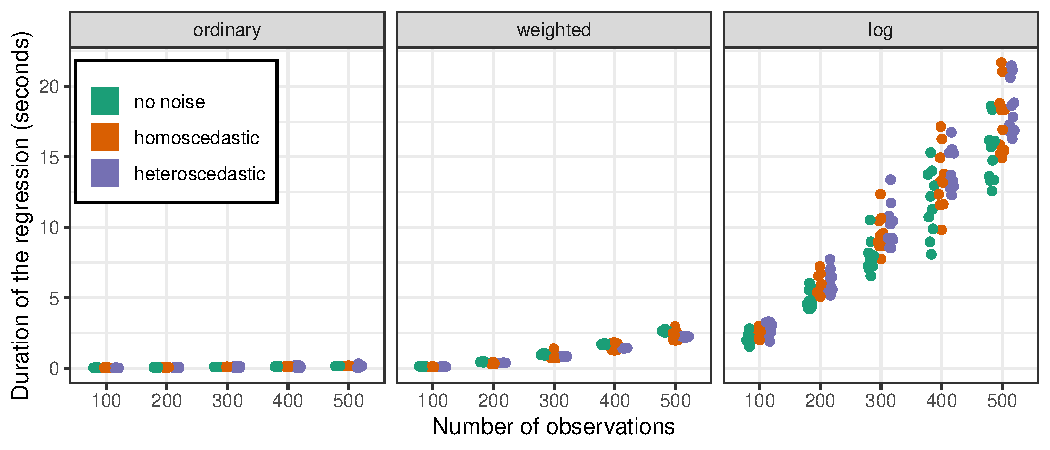
\includegraphics[width=\linewidth]{img/prediction/modeling/network/pycewise_duration.pdf}
                    \caption{Duration of a complete regression with pycewise for different numbers of observations.}%
                    \label{fig:prediction:pycewise_duration}
                \end{figure}

                In our context of network calibration, each communication for a given message size is repeated several
                time. Then, to generate a model, we start by averaging the durations per message size before doing the
                regression, as discussed previously. We can therefore safely expect to have only a few hundreds of
                observations: the logarithmic approach is perfectly reasonable.

    \section{Conclusion}%
        %% TODO
        %% - Formalisme Bayesian Sampling STAN intéressant mais rarement
        %%   applicable directement avec nos données. Besoin de solutions un peu
        %%   ad hoc.
        %% - Note: le fit dépendra des données fournies, d'où l'importance du
        %%   plan d'expérience choisi. Ça sera discuté en partie...
        %% - Pas parfait, c'est un modèle, mais une fois tout ça posé proprement
        %%   on va pouvoir 1) essayer de trouver le bon niveau de modélisation 2)
        %%   détecter des situations à problème 3) faire du whatif.
        We have presented different models for both the network communications and the computation kernels. One
        diffuclty resides in instanciating the models, \ie computing the best fit for some observations, in the most
        automated way possible. Bayesian formalism is an interesting candidate for such a task. With bayesian sampling
        tools like Stan, we should be able to fit arbitrarily complex models and even have an estimation of the
        uncertainty of the resulting paremeters. However, the benefit of these tools is not clear for our context, their
        computation time was particularly slow and we had great difficulties in writing down our models in their
        formalism. In the end, a simpler approach like the method of moments revealed to be enough for our needs.

        The model instance, \ie the fit we compute, will obviously depend on the input data. The experimental protocol
        for collecting the said data will therefore be as important as the statistical tools. This will be further
        discussed in Part~\ref{part:experiment}.

        No model can capture the complexity of the real world perfectly. In Chapter~\ref{chapter:prediction:validation},
        we will discuss what level of complexity is required for achieving a sufficiently faithful performance
        prediction. We will also demonstrate in Chapter~\ref{chapter:prediction:sensibility} how these models can be
        used for sensibility analysis.


\chapter{Validation}%
\label{chapter:prediction:validation}

    \section{Experimental setup}%
    \label{sec:experimental_setup}
        To evaluate the soundness of our approach, we compare several real executions of HPL with simulations using the
        previous models.  We used the Dahu cluster from the Grid'5000 testbed. It has 32 nodes connected through a
        single switch by \SI{100}{\giga\bit\per\second} Omnipath links. Each node has two Intel Xeon Gold 6130 CPU with
        16 cores per CPU and we disabled hyperthreading.  We used HPL version 2.2 compiled with GCC version 6.3.0. We
        also used the libraries OpenMPI version 2.0.2 and OpenBLAS version 0.3.1. We used one single-threaded
        MPI rank per core.

        Although this machine is much smaller than top supercomputers,  faithfully simulating an HPL execution with such
        settings is already quite challenging.
        \begin{itemize}
        \item We used one rank per core to obtain a higher number (1024) of MPI process. This is more difficult than
            simulating one rank per node, as (1) this increases the amount of data transferred through MPI and (2) the
            performance is then subject to memory interference and network heterogeneity (we used a different model for
            local and remote communications).
        \item We used a smaller block size than commonly used, which leads to a higher number of iterations and hence
            more complex communication patterns.
        \item We used relatively small input matrices, which reduces the makespan and makes good predictions harder to
            obtain.
        \end{itemize}

    \section{Different problem sizes}%
    \label{sec:different_problem_sizes}
        %% TODO Importance du modlèe dgemm. Validation qualitative (Gantt chart) et quantitative (scatter plot).

        In this section, HPL executions were done using a block size of 128 and a matrix of varying size (from
        \num{50000} to \num{500000}). We used a a look-ahead \texttt{depth} of 1, the \texttt{increasing-2-ring}
        broadcast with the \texttt{Crout} panel factorization algorithms.

        Our first evaluation consists in comparing the traces of the simulations with reality. We instrumented HPL to
        collect the start and end timestamps of each kernel and MPI call. We limited the execution to 256 ranks and the
        first five iterations.  A first qualitative validation can be done by visually comparing the Gantt charts of the
        simulations with reality (see Figure~\ref{fig:gantt_simulation}). Calls to \dgemm are depicted in yellow, \send
        in red, \recv in blue. Although the structure is similar in all charts, the shape and the duration of the
        communication phases can be overly optimistic in simulations compared to reality.  The charts show that, at this
        scale, using a deterministic or a stochastic model for the network has no noticeable impact on HPL simulation.
        However, having a more complex model for the kernels leads to much more realistic traces. The variability in the
        computation durations leads to an increase of the time spent in communications and an overall slightly longer
        execution. In HPL, computation variability directly translates to late senders/receivers that destroy the
        efficiency of collective operations.

        \newcommand{\ganttcaption}[2]{\rotatebox{90}{\hspace{.6cm}$\text{#1}\atop \text{#2}$\hspace{-1cm}}}
        \begin{figure}[htpb]
            \centering
            \begin{tabular}{c@{}c}
            \ganttcaption{\hspace{.3cm}Reality}{}                        &
            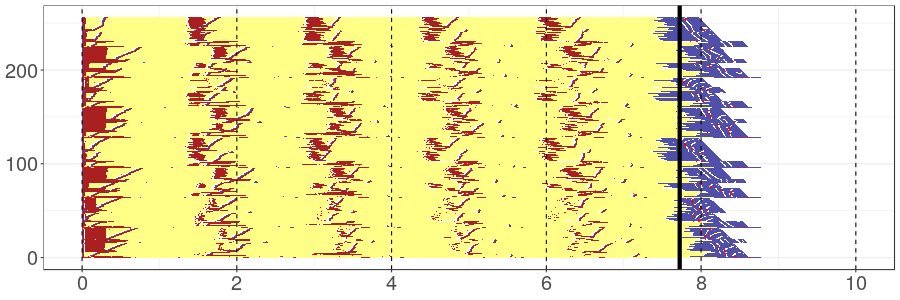
\includegraphics[width=.93\linewidth]{img/prediction/validation/traces/gantt_reality.png} \\
            \ganttcaption{Simple kernel}{Simple network}    &
            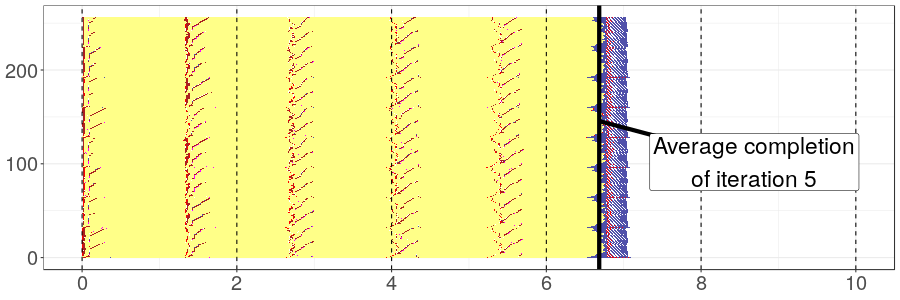
\includegraphics[width=.93\linewidth]{img/prediction/validation/traces/gantt_simulation_deterministic-CPU_linear-DGEMM_deterministic-network.png}\\
            \ganttcaption{Complex kernel}{Simple network}   &
            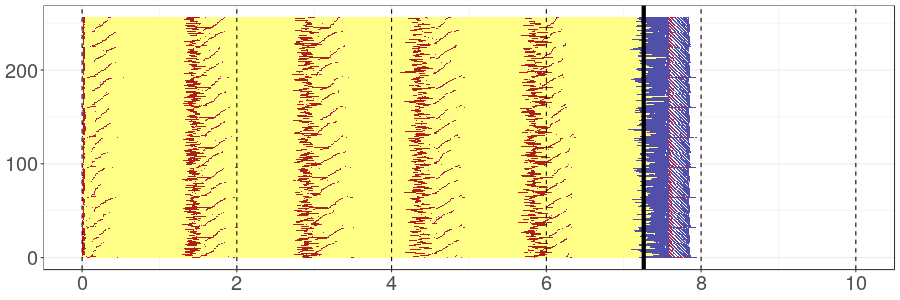
\includegraphics[width=.93\linewidth]{img/prediction/validation/traces/gantt_simulation_stochastic-CPU_polynomial-DGEMM_deterministic-network.png}\\
            \ganttcaption{Complex kernel}{Complex network}  &
            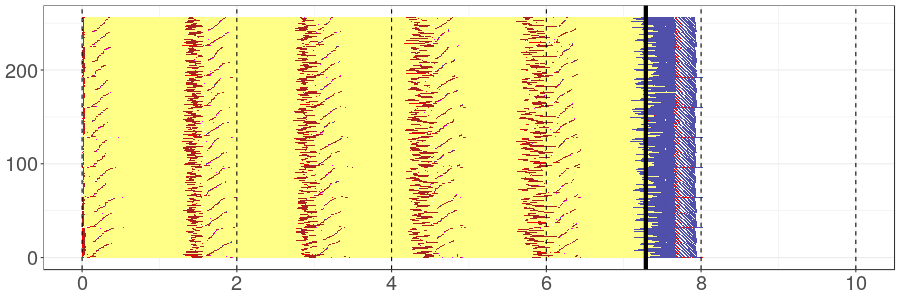
\includegraphics[width=.93\linewidth]{img/prediction/validation/traces/gantt_simulation_stochastic-CPU_polynomial-DGEMM_stochastic-network.png}\\
            \end{tabular}
            \caption{Gantt charts of HPL first iterations in simulation}\vspace{-1em}
            \label{fig:gantt_simulation}
        \end{figure}

        We now provide a more quantitative comparison using the whole cluster and varying matrix sizes, focusing on the
        \si{\giga\flops} rate reported by HPL (see Figure\ref{fig:validation_performance}).  The real executions are
        depicted in black, for each matrix size we performed 8 runs of HPL, to illustrate the temporal variability of
        the performance.  The line (a), on the top, is our first attempt to simulate HPL. The simulation was done with a
        simple model: \model{1} for the kernels and \modelp{1} for the network with no noise (\noise{0}) in both cases.
        This model overestimates HPL performance by more than \SI{30}{\percent}. We initially thought that the network
        model was too optimistic, however, switching to a stochastic multi-modal network model (\noisep{1}, the line
        (b)), does not significantly improve the prediction precision.

        Figure \ref{fig:blas_var} shows that there is an important heterogeneity in the cluster. For this reason, we
        started using a \model[H]{1}/\noise{0} model for \dgemm while keeping the models for the other kernels and the
        network as before. This increases very significantly the realism of the simulation as the performance is now
        overestimated by only \SI{9}{\percent} (the line (c)).  Using a polynomial model for \dgemm instead of a linear
        model (thus switching from \model[H]{1} to \model[H]{2}) further improves the performance prediction, in
        particular for smaller matrices.  This new model (the line (d)), is very close to reality at the beginning but
        becomes equivalent to the previous model for larger matrices.  We found that adding the temporal variability
        noise (\noise{2} for all kernels, \noise[H]{2} for \dgemm) is the key ingredient to obtain the last bit of
        realism. The prediction (the line (e)) is now extremely close to reality as it slightly underestimates the
        performance by less than \SI{5}{\percent} and even as little as \SI{1}{\percent} for the larger matrices. Adding
        back temporal variability to the network model (\noisep{1}, line (f)) still has no significant effect but this
        can be explained by the fact that HPL mostly communicates very large amounts of data in bulk. Network temporal
        variability is however very important aspect to model for applications that are more \emph{latency-bound}.

        \tikzstyle{model_label}=[anchor=south west, font=\scriptsize]
        \begin{figure}[htpb]
            \centering
            \begin{minipage}{0.8\linewidth}
                \begin{tikzpicture}
                    \node[anchor=south west,inner sep=0] at (0,0)
                    {\hbox{\hspace{-.05\linewidth}\resizebox{\linewidth}{!}{% Created by tikzDevice version 0.12 on 2021-06-19 15:41:28
% !TEX encoding = UTF-8 Unicode
\begin{tikzpicture}[x=1pt,y=1pt]
\definecolor{fillColor}{RGB}{255,255,255}
\path[use as bounding box,fill=fillColor,fill opacity=0.00] (0,0) rectangle (361.35,216.81);
\begin{scope}
\path[clip] (  0.00,  0.00) rectangle (361.35,216.81);
\definecolor{drawColor}{RGB}{255,255,255}
\definecolor{fillColor}{RGB}{255,255,255}

\path[draw=drawColor,line width= 0.6pt,line join=round,line cap=round,fill=fillColor] (  0.00,  0.00) rectangle (361.35,216.81);
\end{scope}
\begin{scope}
\path[clip] ( 44.91, 30.69) rectangle (355.85,211.31);
\definecolor{fillColor}{RGB}{255,255,255}

\path[fill=fillColor] ( 44.91, 30.69) rectangle (355.85,211.31);
\definecolor{drawColor}{gray}{0.92}

\path[draw=drawColor,line width= 0.3pt,line join=round] ( 44.91, 66.75) --
	(355.85, 66.75);

\path[draw=drawColor,line width= 0.3pt,line join=round] ( 44.91,122.45) --
	(355.85,122.45);

\path[draw=drawColor,line width= 0.3pt,line join=round] ( 44.91,178.15) --
	(355.85,178.15);

\path[draw=drawColor,line width= 0.3pt,line join=round] ( 59.04, 30.69) --
	( 59.04,211.31);

\path[draw=drawColor,line width= 0.3pt,line join=round] (117.33, 30.69) --
	(117.33,211.31);

\path[draw=drawColor,line width= 0.3pt,line join=round] (175.61, 30.69) --
	(175.61,211.31);

\path[draw=drawColor,line width= 0.3pt,line join=round] (233.89, 30.69) --
	(233.89,211.31);

\path[draw=drawColor,line width= 0.3pt,line join=round] (292.18, 30.69) --
	(292.18,211.31);

\path[draw=drawColor,line width= 0.3pt,line join=round] (350.46, 30.69) --
	(350.46,211.31);

\path[draw=drawColor,line width= 0.6pt,line join=round] ( 44.91, 38.90) --
	(355.85, 38.90);

\path[draw=drawColor,line width= 0.6pt,line join=round] ( 44.91, 94.60) --
	(355.85, 94.60);

\path[draw=drawColor,line width= 0.6pt,line join=round] ( 44.91,150.30) --
	(355.85,150.30);

\path[draw=drawColor,line width= 0.6pt,line join=round] ( 44.91,206.00) --
	(355.85,206.00);

\path[draw=drawColor,line width= 0.6pt,line join=round] ( 88.18, 30.69) --
	( 88.18,211.31);

\path[draw=drawColor,line width= 0.6pt,line join=round] (146.47, 30.69) --
	(146.47,211.31);

\path[draw=drawColor,line width= 0.6pt,line join=round] (204.75, 30.69) --
	(204.75,211.31);

\path[draw=drawColor,line width= 0.6pt,line join=round] (263.03, 30.69) --
	(263.03,211.31);

\path[draw=drawColor,line width= 0.6pt,line join=round] (321.32, 30.69) --
	(321.32,211.31);
\definecolor{drawColor}{RGB}{0,0,0}

\path[draw=drawColor,line width= 0.4pt,line join=round,line cap=round] (321.32,163.27) circle (  0.89);

\path[draw=drawColor,line width= 0.4pt,line join=round,line cap=round] ( 59.04,110.08) circle (  0.89);

\path[draw=drawColor,line width= 0.4pt,line join=round,line cap=round] (204.75,156.65) circle (  0.89);

\path[draw=drawColor,line width= 0.4pt,line join=round,line cap=round] (263.03,159.54) circle (  0.89);

\path[draw=drawColor,line width= 0.4pt,line join=round,line cap=round] (117.33,149.79) circle (  0.89);

\path[draw=drawColor,line width= 0.4pt,line join=round,line cap=round] (175.61,153.47) circle (  0.89);

\path[draw=drawColor,line width= 0.4pt,line join=round,line cap=round] (292.18,161.66) circle (  0.89);

\path[draw=drawColor,line width= 0.4pt,line join=round,line cap=round] (233.89,162.22) circle (  0.89);

\path[draw=drawColor,line width= 0.4pt,line join=round,line cap=round] (146.47,153.75) circle (  0.89);

\path[draw=drawColor,line width= 0.4pt,line join=round,line cap=round] ( 88.18,142.16) circle (  0.89);

\path[draw=drawColor,line width= 0.4pt,line join=round,line cap=round] ( 73.61,133.53) circle (  0.89);

\path[draw=drawColor,line width= 0.4pt,line join=round,line cap=round] (102.76,147.18) circle (  0.89);

\path[draw=drawColor,line width= 0.4pt,line join=round,line cap=round] (161.04,157.93) circle (  0.89);

\path[draw=drawColor,line width= 0.4pt,line join=round,line cap=round] ( 73.61,133.36) circle (  0.89);

\path[draw=drawColor,line width= 0.4pt,line join=round,line cap=round] (204.75,160.54) circle (  0.89);

\path[draw=drawColor,line width= 0.4pt,line join=round,line cap=round] (292.18,163.33) circle (  0.89);

\path[draw=drawColor,line width= 0.4pt,line join=round,line cap=round] (146.47,156.59) circle (  0.89);

\path[draw=drawColor,line width= 0.4pt,line join=round,line cap=round] (131.90,147.73) circle (  0.89);

\path[draw=drawColor,line width= 0.4pt,line join=round,line cap=round] ( 59.04,110.14) circle (  0.89);

\path[draw=drawColor,line width= 0.4pt,line join=round,line cap=round] (161.04,160.93) circle (  0.89);

\path[draw=drawColor,line width= 0.4pt,line join=round,line cap=round] (175.61,157.26) circle (  0.89);

\path[draw=drawColor,line width= 0.4pt,line join=round,line cap=round] (102.76,140.94) circle (  0.89);

\path[draw=drawColor,line width= 0.4pt,line join=round,line cap=round] (117.33,146.62) circle (  0.89);

\path[draw=drawColor,line width= 0.4pt,line join=round,line cap=round] ( 88.18,142.44) circle (  0.89);

\path[draw=drawColor,line width= 0.4pt,line join=round,line cap=round] (321.32,162.05) circle (  0.89);

\path[draw=drawColor,line width= 0.4pt,line join=round,line cap=round] (263.03,160.77) circle (  0.89);

\path[draw=drawColor,line width= 0.4pt,line join=round,line cap=round] (233.89,158.71) circle (  0.89);

\path[draw=drawColor,line width= 0.4pt,line join=round,line cap=round] ( 59.04,110.41) circle (  0.89);

\path[draw=drawColor,line width= 0.4pt,line join=round,line cap=round] (102.76,140.77) circle (  0.89);

\path[draw=drawColor,line width= 0.4pt,line join=round,line cap=round] (321.32,160.21) circle (  0.89);

\path[draw=drawColor,line width= 0.4pt,line join=round,line cap=round] (161.04,153.69) circle (  0.89);

\path[draw=drawColor,line width= 0.4pt,line join=round,line cap=round] (117.33,148.90) circle (  0.89);

\path[draw=drawColor,line width= 0.4pt,line join=round,line cap=round] (263.03,159.99) circle (  0.89);

\path[draw=drawColor,line width= 0.4pt,line join=round,line cap=round] ( 73.61,128.68) circle (  0.89);

\path[draw=drawColor,line width= 0.4pt,line join=round,line cap=round] (204.75,158.43) circle (  0.89);

\path[draw=drawColor,line width= 0.4pt,line join=round,line cap=round] (233.89,160.27) circle (  0.89);

\path[draw=drawColor,line width= 0.4pt,line join=round,line cap=round] (292.18,161.27) circle (  0.89);

\path[draw=drawColor,line width= 0.4pt,line join=round,line cap=round] (175.61,154.59) circle (  0.89);

\path[draw=drawColor,line width= 0.4pt,line join=round,line cap=round] (146.47,155.92) circle (  0.89);

\path[draw=drawColor,line width= 0.4pt,line join=round,line cap=round] ( 88.18,135.98) circle (  0.89);

\path[draw=drawColor,line width= 0.4pt,line join=round,line cap=round] (131.90,148.01) circle (  0.89);

\path[draw=drawColor,line width= 0.4pt,line join=round,line cap=round] (175.61,156.31) circle (  0.89);

\path[draw=drawColor,line width= 0.4pt,line join=round,line cap=round] ( 59.04,108.58) circle (  0.89);

\path[draw=drawColor,line width= 0.4pt,line join=round,line cap=round] (204.75,158.37) circle (  0.89);

\path[draw=drawColor,line width= 0.4pt,line join=round,line cap=round] (102.76,141.27) circle (  0.89);

\path[draw=drawColor,line width= 0.4pt,line join=round,line cap=round] ( 88.18,136.71) circle (  0.89);

\path[draw=drawColor,line width= 0.4pt,line join=round,line cap=round] (321.32,162.61) circle (  0.89);

\path[draw=drawColor,line width= 0.4pt,line join=round,line cap=round] ( 73.61,132.14) circle (  0.89);

\path[draw=drawColor,line width= 0.4pt,line join=round,line cap=round] (117.33,145.23) circle (  0.89);

\path[draw=drawColor,line width= 0.4pt,line join=round,line cap=round] (146.47,153.25) circle (  0.89);

\path[draw=drawColor,line width= 0.4pt,line join=round,line cap=round] (263.03,159.99) circle (  0.89);

\path[draw=drawColor,line width= 0.4pt,line join=round,line cap=round] (161.04,155.31) circle (  0.89);

\path[draw=drawColor,line width= 0.4pt,line join=round,line cap=round] (292.18,159.38) circle (  0.89);

\path[draw=drawColor,line width= 0.4pt,line join=round,line cap=round] (131.90,148.24) circle (  0.89);

\path[draw=drawColor,line width= 0.4pt,line join=round,line cap=round] (233.89,159.65) circle (  0.89);

\path[draw=drawColor,line width= 0.4pt,line join=round,line cap=round] (146.47,150.85) circle (  0.89);

\path[draw=drawColor,line width= 0.4pt,line join=round,line cap=round] (292.18,160.21) circle (  0.89);

\path[draw=drawColor,line width= 0.4pt,line join=round,line cap=round] (131.90,149.85) circle (  0.89);

\path[draw=drawColor,line width= 0.4pt,line join=round,line cap=round] (263.03,158.43) circle (  0.89);

\path[draw=drawColor,line width= 0.4pt,line join=round,line cap=round] (175.61,155.42) circle (  0.89);

\path[draw=drawColor,line width= 0.4pt,line join=round,line cap=round] ( 59.04,111.08) circle (  0.89);

\path[draw=drawColor,line width= 0.4pt,line join=round,line cap=round] (204.75,158.82) circle (  0.89);

\path[draw=drawColor,line width= 0.4pt,line join=round,line cap=round] (321.32,159.88) circle (  0.89);

\path[draw=drawColor,line width= 0.4pt,line join=round,line cap=round] ( 73.61,133.14) circle (  0.89);

\path[draw=drawColor,line width= 0.4pt,line join=round,line cap=round] (102.76,147.62) circle (  0.89);

\path[draw=drawColor,line width= 0.4pt,line join=round,line cap=round] (117.33,151.08) circle (  0.89);

\path[draw=drawColor,line width= 0.4pt,line join=round,line cap=round] ( 88.18,135.15) circle (  0.89);

\path[draw=drawColor,line width= 0.4pt,line join=round,line cap=round] (161.04,154.31) circle (  0.89);

\path[draw=drawColor,line width= 0.4pt,line join=round,line cap=round] (233.89,158.54) circle (  0.89);

\path[draw=drawColor,line width= 0.4pt,line join=round,line cap=round] (321.32,160.77) circle (  0.89);

\path[draw=drawColor,line width= 0.4pt,line join=round,line cap=round] ( 59.04,110.19) circle (  0.89);

\path[draw=drawColor,line width= 0.4pt,line join=round,line cap=round] (204.75,156.70) circle (  0.89);

\path[draw=drawColor,line width= 0.4pt,line join=round,line cap=round] (263.03,159.32) circle (  0.89);

\path[draw=drawColor,line width= 0.4pt,line join=round,line cap=round] (117.33,145.73) circle (  0.89);

\path[draw=drawColor,line width= 0.4pt,line join=round,line cap=round] (175.61,156.98) circle (  0.89);

\path[draw=drawColor,line width= 0.4pt,line join=round,line cap=round] (292.18,160.27) circle (  0.89);

\path[draw=drawColor,line width= 0.4pt,line join=round,line cap=round] (233.89,159.54) circle (  0.89);

\path[draw=drawColor,line width= 0.4pt,line join=round,line cap=round] (146.47,150.35) circle (  0.89);

\path[draw=drawColor,line width= 0.4pt,line join=round,line cap=round] ( 88.18,136.26) circle (  0.89);

\path[draw=drawColor,line width= 0.4pt,line join=round,line cap=round] ( 73.61,130.24) circle (  0.89);

\path[draw=drawColor,line width= 0.4pt,line join=round,line cap=round] (102.76,147.68) circle (  0.89);

\path[draw=drawColor,line width= 0.4pt,line join=round,line cap=round] (161.04,157.15) circle (  0.89);

\path[draw=drawColor,line width= 0.4pt,line join=round,line cap=round] ( 73.61,127.29) circle (  0.89);

\path[draw=drawColor,line width= 0.4pt,line join=round,line cap=round] (204.75,159.99) circle (  0.89);

\path[draw=drawColor,line width= 0.4pt,line join=round,line cap=round] (292.18,159.99) circle (  0.89);

\path[draw=drawColor,line width= 0.4pt,line join=round,line cap=round] (146.47,152.19) circle (  0.89);

\path[draw=drawColor,line width= 0.4pt,line join=round,line cap=round] (131.90,153.81) circle (  0.89);

\path[draw=drawColor,line width= 0.4pt,line join=round,line cap=round] ( 59.04,110.41) circle (  0.89);

\path[draw=drawColor,line width= 0.4pt,line join=round,line cap=round] (161.04,152.86) circle (  0.89);

\path[draw=drawColor,line width= 0.4pt,line join=round,line cap=round] (175.61,152.91) circle (  0.89);

\path[draw=drawColor,line width= 0.4pt,line join=round,line cap=round] (102.76,143.50) circle (  0.89);

\path[draw=drawColor,line width= 0.4pt,line join=round,line cap=round] (117.33,143.45) circle (  0.89);

\path[draw=drawColor,line width= 0.4pt,line join=round,line cap=round] ( 88.18,136.37) circle (  0.89);

\path[draw=drawColor,line width= 0.4pt,line join=round,line cap=round] (321.32,161.05) circle (  0.89);

\path[draw=drawColor,line width= 0.4pt,line join=round,line cap=round] (263.03,160.43) circle (  0.89);

\path[draw=drawColor,line width= 0.4pt,line join=round,line cap=round] (233.89,160.88) circle (  0.89);

\path[draw=drawColor,line width= 0.4pt,line join=round,line cap=round] ( 59.04,110.53) circle (  0.89);

\path[draw=drawColor,line width= 0.4pt,line join=round,line cap=round] (102.76,142.22) circle (  0.89);

\path[draw=drawColor,line width= 0.4pt,line join=round,line cap=round] (321.32,161.83) circle (  0.89);

\path[draw=drawColor,line width= 0.4pt,line join=round,line cap=round] (161.04,157.76) circle (  0.89);

\path[draw=drawColor,line width= 0.4pt,line join=round,line cap=round] (117.33,145.00) circle (  0.89);

\path[draw=drawColor,line width= 0.4pt,line join=round,line cap=round] (263.03,159.04) circle (  0.89);

\path[draw=drawColor,line width= 0.4pt,line join=round,line cap=round] ( 73.61,131.97) circle (  0.89);

\path[draw=drawColor,line width= 0.4pt,line join=round,line cap=round] (204.75,159.32) circle (  0.89);

\path[draw=drawColor,line width= 0.4pt,line join=round,line cap=round] (233.89,161.21) circle (  0.89);

\path[draw=drawColor,line width= 0.4pt,line join=round,line cap=round] (292.18,160.66) circle (  0.89);

\path[draw=drawColor,line width= 0.4pt,line join=round,line cap=round] (175.61,158.37) circle (  0.89);

\path[draw=drawColor,line width= 0.4pt,line join=round,line cap=round] (146.47,156.37) circle (  0.89);

\path[draw=drawColor,line width= 0.4pt,line join=round,line cap=round] ( 88.18,140.44) circle (  0.89);

\path[draw=drawColor,line width= 0.4pt,line join=round,line cap=round] (131.90,147.57) circle (  0.89);
\definecolor{drawColor}{RGB}{230,171,2}
\definecolor{fillColor}{RGB}{230,171,2}

\path[draw=drawColor,line width= 0.4pt,line join=round,line cap=round,fill=fillColor] ( 73.61,127.63) circle (  0.89);

\path[draw=drawColor,line width= 0.4pt,line join=round,line cap=round,fill=fillColor] (131.90,148.57) circle (  0.89);

\path[draw=drawColor,line width= 0.4pt,line join=round,line cap=round,fill=fillColor] (233.89,158.48) circle (  0.89);
\definecolor{drawColor}{RGB}{217,95,2}
\definecolor{fillColor}{RGB}{217,95,2}

\path[draw=drawColor,line width= 0.4pt,line join=round,line cap=round,fill=fillColor] ( 59.04,116.32) circle (  0.89);

\path[draw=drawColor,line width= 0.4pt,line join=round,line cap=round,fill=fillColor] (117.33,153.14) circle (  0.89);

\path[draw=drawColor,line width= 0.4pt,line join=round,line cap=round,fill=fillColor] (204.75,167.84) circle (  0.89);

\path[draw=drawColor,line width= 0.4pt,line join=round,line cap=round,fill=fillColor] (321.32,172.07) circle (  0.89);
\definecolor{drawColor}{RGB}{230,171,2}
\definecolor{fillColor}{RGB}{230,171,2}

\path[draw=drawColor,line width= 0.4pt,line join=round,line cap=round,fill=fillColor] ( 88.18,137.49) circle (  0.89);

\path[draw=drawColor,line width= 0.4pt,line join=round,line cap=round,fill=fillColor] (146.47,151.02) circle (  0.89);

\path[draw=drawColor,line width= 0.4pt,line join=round,line cap=round,fill=fillColor] (263.03,158.04) circle (  0.89);

\path[draw=drawColor,line width= 0.4pt,line join=round,line cap=round,fill=fillColor] ( 59.04,111.42) circle (  0.89);

\path[draw=drawColor,line width= 0.4pt,line join=round,line cap=round,fill=fillColor] (117.33,145.00) circle (  0.89);

\path[draw=drawColor,line width= 0.4pt,line join=round,line cap=round,fill=fillColor] (204.75,157.37) circle (  0.89);

\path[draw=drawColor,line width= 0.4pt,line join=round,line cap=round,fill=fillColor] (321.32,160.10) circle (  0.89);
\definecolor{drawColor}{RGB}{231,41,138}
\definecolor{fillColor}{RGB}{231,41,138}

\path[draw=drawColor,line width= 0.4pt,line join=round,line cap=round,fill=fillColor] ( 73.61,130.91) circle (  0.89);

\path[draw=drawColor,line width= 0.4pt,line join=round,line cap=round,fill=fillColor] (131.90,154.42) circle (  0.89);

\path[draw=drawColor,line width= 0.4pt,line join=round,line cap=round,fill=fillColor] (233.89,168.79) circle (  0.89);
\definecolor{drawColor}{RGB}{102,166,30}
\definecolor{fillColor}{RGB}{102,166,30}

\path[draw=drawColor,line width= 0.4pt,line join=round,line cap=round,fill=fillColor] ( 59.04,112.36) circle (  0.89);

\path[draw=drawColor,line width= 0.4pt,line join=round,line cap=round,fill=fillColor] (117.33,144.95) circle (  0.89);

\path[draw=drawColor,line width= 0.4pt,line join=round,line cap=round,fill=fillColor] (204.75,156.70) circle (  0.89);

\path[draw=drawColor,line width= 0.4pt,line join=round,line cap=round,fill=fillColor] (321.32,159.82) circle (  0.89);
\definecolor{drawColor}{RGB}{231,41,138}
\definecolor{fillColor}{RGB}{231,41,138}

\path[draw=drawColor,line width= 0.4pt,line join=round,line cap=round,fill=fillColor] ( 59.04,113.87) circle (  0.89);

\path[draw=drawColor,line width= 0.4pt,line join=round,line cap=round,fill=fillColor] (117.33,150.18) circle (  0.89);

\path[draw=drawColor,line width= 0.4pt,line join=round,line cap=round,fill=fillColor] (204.75,166.39) circle (  0.89);

\path[draw=drawColor,line width= 0.4pt,line join=round,line cap=round,fill=fillColor] (321.32,171.30) circle (  0.89);

\path[draw=drawColor,line width= 0.4pt,line join=round,line cap=round,fill=fillColor] (102.76,144.56) circle (  0.89);

\path[draw=drawColor,line width= 0.4pt,line join=round,line cap=round,fill=fillColor] (175.61,163.00) circle (  0.89);

\path[draw=drawColor,line width= 0.4pt,line join=round,line cap=round,fill=fillColor] (292.18,170.13) circle (  0.89);
\definecolor{drawColor}{RGB}{217,95,2}
\definecolor{fillColor}{RGB}{217,95,2}

\path[draw=drawColor,line width= 0.4pt,line join=round,line cap=round,fill=fillColor] ( 73.61,134.59) circle (  0.89);

\path[draw=drawColor,line width= 0.4pt,line join=round,line cap=round,fill=fillColor] (131.90,157.15) circle (  0.89);

\path[draw=drawColor,line width= 0.4pt,line join=round,line cap=round,fill=fillColor] (233.89,170.07) circle (  0.89);

\path[draw=drawColor,line width= 0.4pt,line join=round,line cap=round,fill=fillColor] (102.76,147.90) circle (  0.89);

\path[draw=drawColor,line width= 0.4pt,line join=round,line cap=round,fill=fillColor] (175.61,164.72) circle (  0.89);

\path[draw=drawColor,line width= 0.4pt,line join=round,line cap=round,fill=fillColor] (292.18,171.02) circle (  0.89);
\definecolor{drawColor}{RGB}{102,166,30}
\definecolor{fillColor}{RGB}{102,166,30}

\path[draw=drawColor,line width= 0.4pt,line join=round,line cap=round,fill=fillColor] (102.76,140.44) circle (  0.89);

\path[draw=drawColor,line width= 0.4pt,line join=round,line cap=round,fill=fillColor] (175.61,155.25) circle (  0.89);

\path[draw=drawColor,line width= 0.4pt,line join=round,line cap=round,fill=fillColor] (292.18,159.04) circle (  0.89);
\definecolor{drawColor}{RGB}{230,171,2}
\definecolor{fillColor}{RGB}{230,171,2}

\path[draw=drawColor,line width= 0.4pt,line join=round,line cap=round,fill=fillColor] (102.76,140.60) circle (  0.89);

\path[draw=drawColor,line width= 0.4pt,line join=round,line cap=round,fill=fillColor] (175.61,154.70) circle (  0.89);

\path[draw=drawColor,line width= 0.4pt,line join=round,line cap=round,fill=fillColor] (292.18,159.21) circle (  0.89);
\definecolor{drawColor}{RGB}{102,166,30}
\definecolor{fillColor}{RGB}{102,166,30}

\path[draw=drawColor,line width= 0.4pt,line join=round,line cap=round,fill=fillColor] ( 73.61,128.13) circle (  0.89);

\path[draw=drawColor,line width= 0.4pt,line join=round,line cap=round,fill=fillColor] (131.90,148.57) circle (  0.89);

\path[draw=drawColor,line width= 0.4pt,line join=round,line cap=round,fill=fillColor] (233.89,158.32) circle (  0.89);

\path[draw=drawColor,line width= 0.4pt,line join=round,line cap=round,fill=fillColor] ( 88.18,137.76) circle (  0.89);

\path[draw=drawColor,line width= 0.4pt,line join=round,line cap=round,fill=fillColor] (146.47,151.30) circle (  0.89);

\path[draw=drawColor,line width= 0.4pt,line join=round,line cap=round,fill=fillColor] (263.03,158.09) circle (  0.89);
\definecolor{drawColor}{RGB}{217,95,2}
\definecolor{fillColor}{RGB}{217,95,2}

\path[draw=drawColor,line width= 0.4pt,line join=round,line cap=round,fill=fillColor] ( 88.18,144.89) circle (  0.89);

\path[draw=drawColor,line width= 0.4pt,line join=round,line cap=round,fill=fillColor] (146.47,160.21) circle (  0.89);

\path[draw=drawColor,line width= 0.4pt,line join=round,line cap=round,fill=fillColor] (263.03,169.68) circle (  0.89);
\definecolor{drawColor}{RGB}{231,41,138}
\definecolor{fillColor}{RGB}{231,41,138}

\path[draw=drawColor,line width= 0.4pt,line join=round,line cap=round,fill=fillColor] ( 88.18,141.33) circle (  0.89);

\path[draw=drawColor,line width= 0.4pt,line join=round,line cap=round,fill=fillColor] (146.47,157.82) circle (  0.89);

\path[draw=drawColor,line width= 0.4pt,line join=round,line cap=round,fill=fillColor] (263.03,168.62) circle (  0.89);
\definecolor{drawColor}{RGB}{27,158,119}
\definecolor{fillColor}{RGB}{27,158,119}

\path[draw=drawColor,line width= 0.4pt,line join=round,line cap=round,fill=fillColor] (321.32,201.99) circle (  0.89);

\path[draw=drawColor,line width= 0.4pt,line join=round,line cap=round,fill=fillColor] ( 59.04,119.38) circle (  0.89);

\path[draw=drawColor,line width= 0.4pt,line join=round,line cap=round,fill=fillColor] (204.75,192.85) circle (  0.89);

\path[draw=drawColor,line width= 0.4pt,line join=round,line cap=round,fill=fillColor] (263.03,198.48) circle (  0.89);

\path[draw=drawColor,line width= 0.4pt,line join=round,line cap=round,fill=fillColor] (117.33,172.02) circle (  0.89);

\path[draw=drawColor,line width= 0.4pt,line join=round,line cap=round,fill=fillColor] (146.47,181.93) circle (  0.89);

\path[draw=drawColor,line width= 0.4pt,line join=round,line cap=round,fill=fillColor] ( 88.18,155.81) circle (  0.89);

\path[draw=drawColor,line width= 0.4pt,line join=round,line cap=round,fill=fillColor] (131.90,177.48) circle (  0.89);

\path[draw=drawColor,line width= 0.4pt,line join=round,line cap=round,fill=fillColor] (175.61,188.12) circle (  0.89);

\path[draw=drawColor,line width= 0.4pt,line join=round,line cap=round,fill=fillColor] (292.18,200.48) circle (  0.89);

\path[draw=drawColor,line width= 0.4pt,line join=round,line cap=round,fill=fillColor] (233.89,196.08) circle (  0.89);

\path[draw=drawColor,line width= 0.4pt,line join=round,line cap=round,fill=fillColor] ( 73.61,141.89) circle (  0.89);

\path[draw=drawColor,line width= 0.4pt,line join=round,line cap=round,fill=fillColor] (102.76,164.89) circle (  0.89);
\definecolor{drawColor}{RGB}{117,112,179}
\definecolor{fillColor}{RGB}{117,112,179}

\path[draw=drawColor,line width= 0.4pt,line join=round,line cap=round,fill=fillColor] (321.32,201.93) circle (  0.89);

\path[draw=drawColor,line width= 0.4pt,line join=round,line cap=round,fill=fillColor] ( 59.04,118.49) circle (  0.89);

\path[draw=drawColor,line width= 0.4pt,line join=round,line cap=round,fill=fillColor] (204.75,192.74) circle (  0.89);

\path[draw=drawColor,line width= 0.4pt,line join=round,line cap=round,fill=fillColor] (263.03,198.42) circle (  0.89);

\path[draw=drawColor,line width= 0.4pt,line join=round,line cap=round,fill=fillColor] (117.33,171.85) circle (  0.89);

\path[draw=drawColor,line width= 0.4pt,line join=round,line cap=round,fill=fillColor] (146.47,181.77) circle (  0.89);

\path[draw=drawColor,line width= 0.4pt,line join=round,line cap=round,fill=fillColor] ( 88.18,154.92) circle (  0.89);

\path[draw=drawColor,line width= 0.4pt,line join=round,line cap=round,fill=fillColor] (131.90,177.25) circle (  0.89);

\path[draw=drawColor,line width= 0.4pt,line join=round,line cap=round,fill=fillColor] (175.61,188.23) circle (  0.89);

\path[draw=drawColor,line width= 0.4pt,line join=round,line cap=round,fill=fillColor] (292.18,200.48) circle (  0.89);

\path[draw=drawColor,line width= 0.4pt,line join=round,line cap=round,fill=fillColor] (233.89,196.03) circle (  0.89);

\path[draw=drawColor,line width= 0.4pt,line join=round,line cap=round,fill=fillColor] ( 73.61,141.50) circle (  0.89);

\path[draw=drawColor,line width= 0.4pt,line join=round,line cap=round,fill=fillColor] (102.76,164.89) circle (  0.89);
\definecolor{drawColor}{RGB}{27,158,119}

\path[draw=drawColor,line width= 0.6pt,dash pattern=on 4pt off 4pt ,line join=round] ( 59.04,119.38) --
	( 73.61,141.89) --
	( 88.18,155.81) --
	(102.76,164.89) --
	(117.33,172.02) --
	(131.90,177.48) --
	(146.47,181.93) --
	(175.61,188.12) --
	(204.75,192.85) --
	(233.89,196.08) --
	(263.03,198.48) --
	(292.18,200.48) --
	(321.32,201.99);
\definecolor{drawColor}{RGB}{217,95,2}

\path[draw=drawColor,line width= 0.6pt,dash pattern=on 4pt off 4pt ,line join=round] ( 59.04,116.32) --
	( 73.61,134.59) --
	( 88.18,144.89) --
	(102.76,147.90) --
	(117.33,153.14) --
	(131.90,157.15) --
	(146.47,160.21) --
	(175.61,164.72) --
	(204.75,167.84) --
	(233.89,170.07) --
	(263.03,169.68) --
	(292.18,171.02) --
	(321.32,172.07);
\definecolor{drawColor}{RGB}{117,112,179}

\path[draw=drawColor,line width= 0.6pt,dash pattern=on 4pt off 4pt ,line join=round] ( 59.04,118.49) --
	( 73.61,141.50) --
	( 88.18,154.92) --
	(102.76,164.89) --
	(117.33,171.85) --
	(131.90,177.25) --
	(146.47,181.77) --
	(175.61,188.23) --
	(204.75,192.74) --
	(233.89,196.03) --
	(263.03,198.42) --
	(292.18,200.48) --
	(321.32,201.93);
\definecolor{drawColor}{RGB}{231,41,138}

\path[draw=drawColor,line width= 0.6pt,dash pattern=on 4pt off 4pt ,line join=round] ( 59.04,113.87) --
	( 73.61,130.91) --
	( 88.18,141.33) --
	(102.76,144.56) --
	(117.33,150.18) --
	(131.90,154.42) --
	(146.47,157.82) --
	(175.61,163.00) --
	(204.75,166.39) --
	(233.89,168.79) --
	(263.03,168.62) --
	(292.18,170.13) --
	(321.32,171.30);
\definecolor{drawColor}{RGB}{102,166,30}

\path[draw=drawColor,line width= 0.6pt,dash pattern=on 4pt off 4pt ,line join=round] ( 59.04,112.36) --
	( 73.61,128.13) --
	( 88.18,137.76) --
	(102.76,140.44) --
	(117.33,144.95) --
	(131.90,148.57) --
	(146.47,151.30) --
	(175.61,155.25) --
	(204.75,156.70) --
	(233.89,158.32) --
	(263.03,158.09) --
	(292.18,159.04) --
	(321.32,159.82);
\definecolor{drawColor}{RGB}{230,171,2}

\path[draw=drawColor,line width= 0.6pt,dash pattern=on 4pt off 4pt ,line join=round] ( 59.04,111.42) --
	( 73.61,127.63) --
	( 88.18,137.49) --
	(102.76,140.60) --
	(117.33,145.00) --
	(131.90,148.57) --
	(146.47,151.02) --
	(175.61,154.70) --
	(204.75,157.37) --
	(233.89,158.48) --
	(263.03,158.04) --
	(292.18,159.21) --
	(321.32,160.10);
\definecolor{drawColor}{RGB}{0,0,0}

\path[draw=drawColor,line width= 0.6pt,line join=round] ( 59.04,110.18) --
	( 73.61,131.30) --
	( 88.18,138.19) --
	(102.76,143.90) --
	(117.33,146.98) --
	(131.90,149.20) --
	(146.47,153.66) --
	(161.04,156.24) --
	(175.61,155.66) --
	(204.75,158.60) --
	(233.89,160.13) --
	(263.03,159.69) --
	(292.18,160.84) --
	(321.32,161.46);
\definecolor{drawColor}{RGB}{230,171,2}

\path[draw=drawColor,line width= 0.6pt,line join=round] (263.03, 55.20) -- (321.32,160.10);
\definecolor{drawColor}{RGB}{102,166,30}

\path[draw=drawColor,line width= 0.6pt,line join=round] (140.64, 55.20) -- (321.32,159.82);
\definecolor{drawColor}{RGB}{231,41,138}

\path[draw=drawColor,line width= 0.6pt,line join=round] (228.06,104.13) -- (175.61,163.00);
\definecolor{drawColor}{RGB}{217,95,2}

\path[draw=drawColor,line width= 0.6pt,line join=round] (117.33,104.13) -- (175.61,164.72);
\definecolor{drawColor}{RGB}{27,158,119}

\path[draw=drawColor,line width= 0.6pt,line join=round] (102.76,193.83) -- (204.75,192.85);
\definecolor{drawColor}{RGB}{117,112,179}

\path[draw=drawColor,line width= 0.6pt,line join=round] (263.03,185.68) -- (204.75,192.74);
\definecolor{drawColor}{RGB}{255,255,255}
\definecolor{fillColor}{RGB}{255,255,255}

\path[draw=drawColor,line width= 0.3pt,line join=round,line cap=round,fill=fillColor] (216.90, 43.11) --
	(309.17, 43.11) --
	(309.09, 43.11) --
	(309.38, 43.12) --
	(309.67, 43.18) --
	(309.94, 43.28) --
	(310.19, 43.43) --
	(310.42, 43.61) --
	(310.61, 43.83) --
	(310.77, 44.08) --
	(310.88, 44.34) --
	(310.95, 44.63) --
	(310.97, 44.92) --
	(310.97, 44.92) --
	(310.97, 65.49) --
	(310.97, 65.49) --
	(310.95, 65.78) --
	(310.88, 66.07) --
	(310.77, 66.33) --
	(310.61, 66.58) --
	(310.42, 66.80) --
	(310.19, 66.98) --
	(309.94, 67.13) --
	(309.67, 67.23) --
	(309.38, 67.29) --
	(309.17, 67.30) --
	(216.90, 67.30) --
	(217.12, 67.29) --
	(216.83, 67.30) --
	(216.54, 67.26) --
	(216.26, 67.18) --
	(216.00, 67.06) --
	(215.76, 66.89) --
	(215.55, 66.69) --
	(215.37, 66.46) --
	(215.24, 66.20) --
	(215.15, 65.93) --
	(215.10, 65.64) --
	(215.09, 65.49) --
	(215.09, 44.92) --
	(215.10, 45.06) --
	(215.10, 44.77) --
	(215.15, 44.48) --
	(215.24, 44.21) --
	(215.37, 43.95) --
	(215.55, 43.72) --
	(215.76, 43.52) --
	(216.00, 43.35) --
	(216.26, 43.23) --
	(216.54, 43.14) --
	(216.83, 43.11) --
	cycle;
\end{scope}
\begin{scope}
\path[clip] ( 44.91, 30.69) rectangle (355.85,211.31);
\definecolor{drawColor}{RGB}{255,255,255}

\node[text=drawColor,anchor=base,inner sep=0pt, outer sep=0pt, scale=  0.85] at (263.03, 58.41) {\textbf{(f)} model (e) with};

\node[text=drawColor,anchor=base,inner sep=0pt, outer sep=0pt, scale=  0.85] at (263.03, 46.12) {\vspace{1cm} network$\sim\mathbf{M'}\!-\!1 \mathbf{N'}\!-\!1$ \vspace{1cm}};
\definecolor{fillColor}{RGB}{255,255,255}

\path[draw=drawColor,line width= 0.3pt,line join=round,line cap=round,fill=fillColor] ( 91.74, 36.96) --
	(189.54, 36.96) --
	(189.46, 36.96) --
	(189.75, 36.98) --
	(190.04, 37.03) --
	(190.31, 37.14) --
	(190.56, 37.28) --
	(190.79, 37.47) --
	(190.98, 37.68) --
	(191.14, 37.93) --
	(191.25, 38.20) --
	(191.32, 38.48) --
	(191.34, 38.77) --
	(191.34, 38.77) --
	(191.34, 71.64) --
	(191.34, 71.64) --
	(191.32, 71.93) --
	(191.25, 72.21) --
	(191.14, 72.48) --
	(190.98, 72.73) --
	(190.79, 72.94) --
	(190.56, 73.13) --
	(190.31, 73.27) --
	(190.04, 73.38) --
	(189.75, 73.43) --
	(189.54, 73.45) --
	( 91.74, 73.45) --
	( 91.96, 73.43) --
	( 91.67, 73.45) --
	( 91.38, 73.41) --
	( 91.10, 73.33) --
	( 90.84, 73.21) --
	( 90.60, 73.04) --
	( 90.39, 72.84) --
	( 90.22, 72.61) --
	( 90.08, 72.35) --
	( 89.99, 72.07) --
	( 89.94, 71.79) --
	( 89.94, 71.64) --
	( 89.94, 38.77) --
	( 89.94, 38.91) --
	( 89.94, 38.62) --
	( 89.99, 38.34) --
	( 90.08, 38.06) --
	( 90.22, 37.80) --
	( 90.39, 37.57) --
	( 90.60, 37.37) --
	( 90.84, 37.20) --
	( 91.10, 37.08) --
	( 91.38, 37.00) --
	( 91.67, 36.96) --
	cycle;
\end{scope}
\begin{scope}
\path[clip] ( 44.91, 30.69) rectangle (355.85,211.31);
\definecolor{drawColor}{RGB}{255,255,255}

\node[text=drawColor,anchor=base,inner sep=0pt, outer sep=0pt, scale=  0.85] at (140.64, 64.56) {\textbf{(e)} model (a) with};

\node[text=drawColor,anchor=base,inner sep=0pt, outer sep=0pt, scale=  0.85] at (140.64, 52.27) {\vspace{1cm} kernels$\sim\mathbf{M}\!-\!1 \mathbf{N}\!-\!2$ \vspace{1cm}};

\node[text=drawColor,anchor=base,inner sep=0pt, outer sep=0pt, scale=  0.85] at (140.64, 39.97) {\vspace{1cm} dgemm$\sim\mathbf{M}_{H}\!-\!2 \mathbf{N}_{H}\!-\!2$ \vspace{1cm}};
\definecolor{fillColor}{RGB}{255,255,255}

\path[draw=drawColor,line width= 0.3pt,line join=round,line cap=round,fill=fillColor] (182.40, 92.04) --
	(273.72, 92.04) --
	(273.65, 92.04) --
	(273.94, 92.05) --
	(274.23, 92.11) --
	(274.50, 92.21) --
	(274.75, 92.36) --
	(274.98, 92.54) --
	(275.17, 92.76) --
	(275.32, 93.00) --
	(275.44, 93.27) --
	(275.51, 93.55) --
	(275.53, 93.84) --
	(275.53, 93.84) --
	(275.53,114.42) --
	(275.53,114.42) --
	(275.51,114.71) --
	(275.44,114.99) --
	(275.32,115.26) --
	(275.17,115.51) --
	(274.98,115.72) --
	(274.75,115.91) --
	(274.50,116.05) --
	(274.23,116.16) --
	(273.94,116.22) --
	(273.72,116.23) --
	(182.40,116.23) --
	(182.62,116.22) --
	(182.33,116.23) --
	(182.04,116.19) --
	(181.76,116.11) --
	(181.50,115.99) --
	(181.26,115.82) --
	(181.05,115.62) --
	(180.88,115.39) --
	(180.74,115.13) --
	(180.65,114.85) --
	(180.60,114.57) --
	(180.60,114.42) --
	(180.60, 93.84) --
	(180.60, 93.99) --
	(180.60, 93.70) --
	(180.65, 93.41) --
	(180.74, 93.13) --
	(180.88, 92.88) --
	(181.05, 92.64) --
	(181.26, 92.44) --
	(181.50, 92.28) --
	(181.76, 92.15) --
	(182.04, 92.07) --
	(182.33, 92.04) --
	cycle;
\end{scope}
\begin{scope}
\path[clip] ( 44.91, 30.69) rectangle (355.85,211.31);
\definecolor{drawColor}{RGB}{255,255,255}

\node[text=drawColor,anchor=base,inner sep=0pt, outer sep=0pt, scale=  0.85] at (228.06,107.34) {\textbf{(d)} model (a) with};

\node[text=drawColor,anchor=base,inner sep=0pt, outer sep=0pt, scale=  0.85] at (228.06, 95.05) {\vspace{1cm} dgemm$\sim\mathbf{M}_{H}\!-\!2 \mathbf{N}\!-\!0$ \vspace{1cm}};
\definecolor{fillColor}{RGB}{255,255,255}

\path[draw=drawColor,line width= 0.3pt,line join=round,line cap=round,fill=fillColor] ( 71.67, 92.04) --
	(162.99, 92.04) --
	(162.91, 92.04) --
	(163.20, 92.05) --
	(163.49, 92.11) --
	(163.76, 92.21) --
	(164.01, 92.36) --
	(164.24, 92.54) --
	(164.43, 92.76) --
	(164.59, 93.00) --
	(164.70, 93.27) --
	(164.77, 93.55) --
	(164.79, 93.84) --
	(164.79, 93.84) --
	(164.79,114.42) --
	(164.79,114.42) --
	(164.77,114.71) --
	(164.70,114.99) --
	(164.59,115.26) --
	(164.43,115.51) --
	(164.24,115.72) --
	(164.01,115.91) --
	(163.76,116.05) --
	(163.49,116.16) --
	(163.20,116.22) --
	(162.99,116.23) --
	( 71.67,116.23) --
	( 71.88,116.22) --
	( 71.59,116.23) --
	( 71.30,116.19) --
	( 71.03,116.11) --
	( 70.76,115.99) --
	( 70.52,115.82) --
	( 70.31,115.62) --
	( 70.14,115.39) --
	( 70.00,115.13) --
	( 69.91,114.85) --
	( 69.87,114.57) --
	( 69.86,114.42) --
	( 69.86, 93.84) --
	( 69.87, 93.99) --
	( 69.87, 93.70) --
	( 69.91, 93.41) --
	( 70.00, 93.13) --
	( 70.14, 92.88) --
	( 70.31, 92.64) --
	( 70.52, 92.44) --
	( 70.76, 92.28) --
	( 71.03, 92.15) --
	( 71.30, 92.07) --
	( 71.59, 92.04) --
	cycle;
\end{scope}
\begin{scope}
\path[clip] ( 44.91, 30.69) rectangle (355.85,211.31);
\definecolor{drawColor}{RGB}{255,255,255}

\node[text=drawColor,anchor=base,inner sep=0pt, outer sep=0pt, scale=  0.85] at (117.33,107.34) {\textbf{(c)} model (a) with};

\node[text=drawColor,anchor=base,inner sep=0pt, outer sep=0pt, scale=  0.85] at (117.33, 95.05) {\vspace{1cm} dgemm$\sim\mathbf{M}_{H}\!-\!1 \mathbf{N}\!-\!0$ \vspace{1cm}};
\definecolor{fillColor}{RGB}{255,255,255}

\path[draw=drawColor,line width= 0.3pt,line join=round,line cap=round,fill=fillColor] ( 53.38,181.73) --
	(152.13,181.73) --
	(152.05,181.74) --
	(152.34,181.75) --
	(152.63,181.81) --
	(152.90,181.91) --
	(153.15,182.05) --
	(153.38,182.24) --
	(153.57,182.46) --
	(153.73,182.70) --
	(153.84,182.97) --
	(153.91,183.25) --
	(153.93,183.54) --
	(153.93,183.54) --
	(153.93,204.12) --
	(153.93,204.12) --
	(153.91,204.41) --
	(153.84,204.69) --
	(153.73,204.96) --
	(153.57,205.21) --
	(153.38,205.42) --
	(153.15,205.61) --
	(152.90,205.75) --
	(152.63,205.86) --
	(152.34,205.91) --
	(152.13,205.93) --
	( 53.38,205.93) --
	( 53.60,205.91) --
	( 53.31,205.93) --
	( 53.02,205.89) --
	( 52.74,205.81) --
	( 52.48,205.69) --
	( 52.24,205.52) --
	( 52.03,205.32) --
	( 51.86,205.09) --
	( 51.72,204.83) --
	( 51.63,204.55) --
	( 51.58,204.27) --
	( 51.58,204.12) --
	( 51.58,183.54) --
	( 51.58,183.69) --
	( 51.58,183.40) --
	( 51.63,183.11) --
	( 51.72,182.83) --
	( 51.86,182.58) --
	( 52.03,182.34) --
	( 52.24,182.14) --
	( 52.48,181.98) --
	( 52.74,181.85) --
	( 53.02,181.77) --
	( 53.31,181.74) --
	cycle;
\end{scope}
\begin{scope}
\path[clip] ( 44.91, 30.69) rectangle (355.85,211.31);
\definecolor{drawColor}{RGB}{255,255,255}

\node[text=drawColor,anchor=base,inner sep=0pt, outer sep=0pt, scale=  0.85] at (102.76,197.04) {\vspace{1cm} \textbf{(a)} kernels$\sim\mathbf{M}\!-\!1 \mathbf{N}\!-\!0$ \vspace{1cm}};

\node[text=drawColor,anchor=base,inner sep=0pt, outer sep=0pt, scale=  0.85] at (102.76,184.75) {\vspace{1cm} network$\sim\mathbf{M'}\!-\!1 \mathbf{N}\!-\!0$ \vspace{1cm}};
\definecolor{fillColor}{RGB}{255,255,255}

\path[draw=drawColor,line width= 0.3pt,line join=round,line cap=round,fill=fillColor] (216.90,173.58) --
	(309.17,173.58) --
	(309.09,173.58) --
	(309.38,173.59) --
	(309.67,173.65) --
	(309.94,173.75) --
	(310.19,173.90) --
	(310.42,174.08) --
	(310.61,174.30) --
	(310.77,174.55) --
	(310.88,174.81) --
	(310.95,175.10) --
	(310.97,175.39) --
	(310.97,175.39) --
	(310.97,195.97) --
	(310.97,195.97) --
	(310.95,196.26) --
	(310.88,196.54) --
	(310.77,196.81) --
	(310.61,197.05) --
	(310.42,197.27) --
	(310.19,197.45) --
	(309.94,197.60) --
	(309.67,197.70) --
	(309.38,197.76) --
	(309.17,197.77) --
	(216.90,197.77) --
	(217.12,197.76) --
	(216.83,197.77) --
	(216.54,197.74) --
	(216.26,197.66) --
	(216.00,197.53) --
	(215.76,197.37) --
	(215.55,197.16) --
	(215.37,196.93) --
	(215.24,196.67) --
	(215.15,196.40) --
	(215.10,196.11) --
	(215.09,195.97) --
	(215.09,175.39) --
	(215.10,175.53) --
	(215.10,175.24) --
	(215.15,174.95) --
	(215.24,174.68) --
	(215.37,174.42) --
	(215.55,174.19) --
	(215.76,173.99) --
	(216.00,173.82) --
	(216.26,173.70) --
	(216.54,173.62) --
	(216.83,173.58) --
	cycle;
\end{scope}
\begin{scope}
\path[clip] ( 44.91, 30.69) rectangle (355.85,211.31);
\definecolor{drawColor}{RGB}{255,255,255}

\node[text=drawColor,anchor=base,inner sep=0pt, outer sep=0pt, scale=  0.85] at (263.03,188.88) {\textbf{(b)} model (a) with};

\node[text=drawColor,anchor=base,inner sep=0pt, outer sep=0pt, scale=  0.85] at (263.03,176.59) {\vspace{1cm} network$\sim\mathbf{M'}\!-\!1 \mathbf{N'}\!-\!1$ \vspace{1cm}};
\definecolor{drawColor}{RGB}{0,0,0}
\definecolor{fillColor}{RGB}{230,171,2}

\path[draw=drawColor,line width= 0.3pt,line join=round,line cap=round,fill=fillColor,fill opacity=0.30] (216.90, 43.11) --
	(309.17, 43.11) --
	(309.09, 43.11) --
	(309.38, 43.12) --
	(309.67, 43.18) --
	(309.94, 43.28) --
	(310.19, 43.43) --
	(310.42, 43.61) --
	(310.61, 43.83) --
	(310.77, 44.08) --
	(310.88, 44.34) --
	(310.95, 44.63) --
	(310.97, 44.92) --
	(310.97, 44.92) --
	(310.97, 65.49) --
	(310.97, 65.49) --
	(310.95, 65.78) --
	(310.88, 66.07) --
	(310.77, 66.33) --
	(310.61, 66.58) --
	(310.42, 66.80) --
	(310.19, 66.98) --
	(309.94, 67.13) --
	(309.67, 67.23) --
	(309.38, 67.29) --
	(309.17, 67.30) --
	(216.90, 67.30) --
	(217.12, 67.29) --
	(216.83, 67.30) --
	(216.54, 67.26) --
	(216.26, 67.18) --
	(216.00, 67.06) --
	(215.76, 66.89) --
	(215.55, 66.69) --
	(215.37, 66.46) --
	(215.24, 66.20) --
	(215.15, 65.93) --
	(215.10, 65.64) --
	(215.09, 65.49) --
	(215.09, 44.92) --
	(215.10, 45.06) --
	(215.10, 44.77) --
	(215.15, 44.48) --
	(215.24, 44.21) --
	(215.37, 43.95) --
	(215.55, 43.72) --
	(215.76, 43.52) --
	(216.00, 43.35) --
	(216.26, 43.23) --
	(216.54, 43.14) --
	(216.83, 43.11) --
	cycle;
\end{scope}
\begin{scope}
\path[clip] ( 44.91, 30.69) rectangle (355.85,211.31);
\definecolor{drawColor}{RGB}{0,0,0}

\node[text=drawColor,anchor=base,inner sep=0pt, outer sep=0pt, scale=  0.85] at (263.03, 58.41) {\textbf{(f)} model (e) with};

\node[text=drawColor,anchor=base,inner sep=0pt, outer sep=0pt, scale=  0.85] at (263.03, 46.12) {\vspace{1cm} network$\sim\mathbf{M'}\!-\!1 \mathbf{N'}\!-\!1$ \vspace{1cm}};
\definecolor{fillColor}{RGB}{102,166,30}

\path[draw=drawColor,line width= 0.3pt,line join=round,line cap=round,fill=fillColor,fill opacity=0.30] ( 91.74, 36.96) --
	(189.54, 36.96) --
	(189.46, 36.96) --
	(189.75, 36.98) --
	(190.04, 37.03) --
	(190.31, 37.14) --
	(190.56, 37.28) --
	(190.79, 37.47) --
	(190.98, 37.68) --
	(191.14, 37.93) --
	(191.25, 38.20) --
	(191.32, 38.48) --
	(191.34, 38.77) --
	(191.34, 38.77) --
	(191.34, 71.64) --
	(191.34, 71.64) --
	(191.32, 71.93) --
	(191.25, 72.21) --
	(191.14, 72.48) --
	(190.98, 72.73) --
	(190.79, 72.94) --
	(190.56, 73.13) --
	(190.31, 73.27) --
	(190.04, 73.38) --
	(189.75, 73.43) --
	(189.54, 73.45) --
	( 91.74, 73.45) --
	( 91.96, 73.43) --
	( 91.67, 73.45) --
	( 91.38, 73.41) --
	( 91.10, 73.33) --
	( 90.84, 73.21) --
	( 90.60, 73.04) --
	( 90.39, 72.84) --
	( 90.22, 72.61) --
	( 90.08, 72.35) --
	( 89.99, 72.07) --
	( 89.94, 71.79) --
	( 89.94, 71.64) --
	( 89.94, 38.77) --
	( 89.94, 38.91) --
	( 89.94, 38.62) --
	( 89.99, 38.34) --
	( 90.08, 38.06) --
	( 90.22, 37.80) --
	( 90.39, 37.57) --
	( 90.60, 37.37) --
	( 90.84, 37.20) --
	( 91.10, 37.08) --
	( 91.38, 37.00) --
	( 91.67, 36.96) --
	cycle;
\end{scope}
\begin{scope}
\path[clip] ( 44.91, 30.69) rectangle (355.85,211.31);
\definecolor{drawColor}{RGB}{0,0,0}

\node[text=drawColor,anchor=base,inner sep=0pt, outer sep=0pt, scale=  0.85] at (140.64, 64.56) {\textbf{(e)} model (a) with};

\node[text=drawColor,anchor=base,inner sep=0pt, outer sep=0pt, scale=  0.85] at (140.64, 52.27) {\vspace{1cm} kernels$\sim\mathbf{M}\!-\!1 \mathbf{N}\!-\!2$ \vspace{1cm}};

\node[text=drawColor,anchor=base,inner sep=0pt, outer sep=0pt, scale=  0.85] at (140.64, 39.97) {\vspace{1cm} dgemm$\sim\mathbf{M}_{H}\!-\!2 \mathbf{N}_{H}\!-\!2$ \vspace{1cm}};
\definecolor{fillColor}{RGB}{231,41,138}

\path[draw=drawColor,line width= 0.3pt,line join=round,line cap=round,fill=fillColor,fill opacity=0.30] (182.40, 92.04) --
	(273.72, 92.04) --
	(273.65, 92.04) --
	(273.94, 92.05) --
	(274.23, 92.11) --
	(274.50, 92.21) --
	(274.75, 92.36) --
	(274.98, 92.54) --
	(275.17, 92.76) --
	(275.32, 93.00) --
	(275.44, 93.27) --
	(275.51, 93.55) --
	(275.53, 93.84) --
	(275.53, 93.84) --
	(275.53,114.42) --
	(275.53,114.42) --
	(275.51,114.71) --
	(275.44,114.99) --
	(275.32,115.26) --
	(275.17,115.51) --
	(274.98,115.72) --
	(274.75,115.91) --
	(274.50,116.05) --
	(274.23,116.16) --
	(273.94,116.22) --
	(273.72,116.23) --
	(182.40,116.23) --
	(182.62,116.22) --
	(182.33,116.23) --
	(182.04,116.19) --
	(181.76,116.11) --
	(181.50,115.99) --
	(181.26,115.82) --
	(181.05,115.62) --
	(180.88,115.39) --
	(180.74,115.13) --
	(180.65,114.85) --
	(180.60,114.57) --
	(180.60,114.42) --
	(180.60, 93.84) --
	(180.60, 93.99) --
	(180.60, 93.70) --
	(180.65, 93.41) --
	(180.74, 93.13) --
	(180.88, 92.88) --
	(181.05, 92.64) --
	(181.26, 92.44) --
	(181.50, 92.28) --
	(181.76, 92.15) --
	(182.04, 92.07) --
	(182.33, 92.04) --
	cycle;
\end{scope}
\begin{scope}
\path[clip] ( 44.91, 30.69) rectangle (355.85,211.31);
\definecolor{drawColor}{RGB}{0,0,0}

\node[text=drawColor,anchor=base,inner sep=0pt, outer sep=0pt, scale=  0.85] at (228.06,107.34) {\textbf{(d)} model (a) with};

\node[text=drawColor,anchor=base,inner sep=0pt, outer sep=0pt, scale=  0.85] at (228.06, 95.05) {\vspace{1cm} dgemm$\sim\mathbf{M}_{H}\!-\!2 \mathbf{N}\!-\!0$ \vspace{1cm}};
\definecolor{fillColor}{RGB}{217,95,2}

\path[draw=drawColor,line width= 0.3pt,line join=round,line cap=round,fill=fillColor,fill opacity=0.30] ( 71.67, 92.04) --
	(162.99, 92.04) --
	(162.91, 92.04) --
	(163.20, 92.05) --
	(163.49, 92.11) --
	(163.76, 92.21) --
	(164.01, 92.36) --
	(164.24, 92.54) --
	(164.43, 92.76) --
	(164.59, 93.00) --
	(164.70, 93.27) --
	(164.77, 93.55) --
	(164.79, 93.84) --
	(164.79, 93.84) --
	(164.79,114.42) --
	(164.79,114.42) --
	(164.77,114.71) --
	(164.70,114.99) --
	(164.59,115.26) --
	(164.43,115.51) --
	(164.24,115.72) --
	(164.01,115.91) --
	(163.76,116.05) --
	(163.49,116.16) --
	(163.20,116.22) --
	(162.99,116.23) --
	( 71.67,116.23) --
	( 71.88,116.22) --
	( 71.59,116.23) --
	( 71.30,116.19) --
	( 71.03,116.11) --
	( 70.76,115.99) --
	( 70.52,115.82) --
	( 70.31,115.62) --
	( 70.14,115.39) --
	( 70.00,115.13) --
	( 69.91,114.85) --
	( 69.87,114.57) --
	( 69.86,114.42) --
	( 69.86, 93.84) --
	( 69.87, 93.99) --
	( 69.87, 93.70) --
	( 69.91, 93.41) --
	( 70.00, 93.13) --
	( 70.14, 92.88) --
	( 70.31, 92.64) --
	( 70.52, 92.44) --
	( 70.76, 92.28) --
	( 71.03, 92.15) --
	( 71.30, 92.07) --
	( 71.59, 92.04) --
	cycle;
\end{scope}
\begin{scope}
\path[clip] ( 44.91, 30.69) rectangle (355.85,211.31);
\definecolor{drawColor}{RGB}{0,0,0}

\node[text=drawColor,anchor=base,inner sep=0pt, outer sep=0pt, scale=  0.85] at (117.33,107.34) {\textbf{(c)} model (a) with};

\node[text=drawColor,anchor=base,inner sep=0pt, outer sep=0pt, scale=  0.85] at (117.33, 95.05) {\vspace{1cm} dgemm$\sim\mathbf{M}_{H}\!-\!1 \mathbf{N}\!-\!0$ \vspace{1cm}};
\definecolor{fillColor}{RGB}{27,158,119}

\path[draw=drawColor,line width= 0.3pt,line join=round,line cap=round,fill=fillColor,fill opacity=0.30] ( 53.38,181.73) --
	(152.13,181.73) --
	(152.05,181.74) --
	(152.34,181.75) --
	(152.63,181.81) --
	(152.90,181.91) --
	(153.15,182.05) --
	(153.38,182.24) --
	(153.57,182.46) --
	(153.73,182.70) --
	(153.84,182.97) --
	(153.91,183.25) --
	(153.93,183.54) --
	(153.93,183.54) --
	(153.93,204.12) --
	(153.93,204.12) --
	(153.91,204.41) --
	(153.84,204.69) --
	(153.73,204.96) --
	(153.57,205.21) --
	(153.38,205.42) --
	(153.15,205.61) --
	(152.90,205.75) --
	(152.63,205.86) --
	(152.34,205.91) --
	(152.13,205.93) --
	( 53.38,205.93) --
	( 53.60,205.91) --
	( 53.31,205.93) --
	( 53.02,205.89) --
	( 52.74,205.81) --
	( 52.48,205.69) --
	( 52.24,205.52) --
	( 52.03,205.32) --
	( 51.86,205.09) --
	( 51.72,204.83) --
	( 51.63,204.55) --
	( 51.58,204.27) --
	( 51.58,204.12) --
	( 51.58,183.54) --
	( 51.58,183.69) --
	( 51.58,183.40) --
	( 51.63,183.11) --
	( 51.72,182.83) --
	( 51.86,182.58) --
	( 52.03,182.34) --
	( 52.24,182.14) --
	( 52.48,181.98) --
	( 52.74,181.85) --
	( 53.02,181.77) --
	( 53.31,181.74) --
	cycle;
\end{scope}
\begin{scope}
\path[clip] ( 44.91, 30.69) rectangle (355.85,211.31);
\definecolor{drawColor}{RGB}{0,0,0}

\node[text=drawColor,anchor=base,inner sep=0pt, outer sep=0pt, scale=  0.85] at (102.76,197.04) {\vspace{1cm} \textbf{(a)} kernels$\sim\mathbf{M}\!-\!1 \mathbf{N}\!-\!0$ \vspace{1cm}};

\node[text=drawColor,anchor=base,inner sep=0pt, outer sep=0pt, scale=  0.85] at (102.76,184.75) {\vspace{1cm} network$\sim\mathbf{M'}\!-\!1 \mathbf{N}\!-\!0$ \vspace{1cm}};
\definecolor{fillColor}{RGB}{117,112,179}

\path[draw=drawColor,line width= 0.3pt,line join=round,line cap=round,fill=fillColor,fill opacity=0.30] (216.90,173.58) --
	(309.17,173.58) --
	(309.09,173.58) --
	(309.38,173.59) --
	(309.67,173.65) --
	(309.94,173.75) --
	(310.19,173.90) --
	(310.42,174.08) --
	(310.61,174.30) --
	(310.77,174.55) --
	(310.88,174.81) --
	(310.95,175.10) --
	(310.97,175.39) --
	(310.97,175.39) --
	(310.97,195.97) --
	(310.97,195.97) --
	(310.95,196.26) --
	(310.88,196.54) --
	(310.77,196.81) --
	(310.61,197.05) --
	(310.42,197.27) --
	(310.19,197.45) --
	(309.94,197.60) --
	(309.67,197.70) --
	(309.38,197.76) --
	(309.17,197.77) --
	(216.90,197.77) --
	(217.12,197.76) --
	(216.83,197.77) --
	(216.54,197.74) --
	(216.26,197.66) --
	(216.00,197.53) --
	(215.76,197.37) --
	(215.55,197.16) --
	(215.37,196.93) --
	(215.24,196.67) --
	(215.15,196.40) --
	(215.10,196.11) --
	(215.09,195.97) --
	(215.09,175.39) --
	(215.10,175.53) --
	(215.10,175.24) --
	(215.15,174.95) --
	(215.24,174.68) --
	(215.37,174.42) --
	(215.55,174.19) --
	(215.76,173.99) --
	(216.00,173.82) --
	(216.26,173.70) --
	(216.54,173.62) --
	(216.83,173.58) --
	cycle;
\end{scope}
\begin{scope}
\path[clip] ( 44.91, 30.69) rectangle (355.85,211.31);
\definecolor{drawColor}{RGB}{0,0,0}

\node[text=drawColor,anchor=base,inner sep=0pt, outer sep=0pt, scale=  0.85] at (263.03,188.88) {\textbf{(b)} model (a) with};

\node[text=drawColor,anchor=base,inner sep=0pt, outer sep=0pt, scale=  0.85] at (263.03,176.59) {\vspace{1cm} network$\sim\mathbf{M'}\!-\!1 \mathbf{N'}\!-\!1$ \vspace{1cm}};

\path[draw=drawColor,line width= 0.6pt,line join=round] (248.46,136.75) -- (292.18,160.84);

\path[draw=drawColor,line width= 0.6pt,line join=round] (248.46,136.75) -- (292.18,160.84);

\path[draw=drawColor,line width= 0.6pt,line join=round] (248.46,136.75) -- (292.18,160.84);

\path[draw=drawColor,line width= 0.6pt,line join=round] (248.46,136.75) -- (292.18,160.84);

\path[draw=drawColor,line width= 0.6pt,line join=round] (248.46,136.75) -- (292.18,160.84);

\path[draw=drawColor,line width= 0.6pt,line join=round] (248.46,136.75) -- (292.18,160.84);
\definecolor{fillColor}{RGB}{255,255,255}

\path[draw=drawColor,line width= 0.3pt,line join=round,line cap=round,fill=fillColor] (233.45,130.80) --
	(263.48,130.80) --
	(263.41,130.80) --
	(263.70,130.81) --
	(263.98,130.87) --
	(264.25,130.97) --
	(264.51,131.12) --
	(264.73,131.30) --
	(264.92,131.52) --
	(265.08,131.77) --
	(265.19,132.03) --
	(265.26,132.32) --
	(265.29,132.61) --
	(265.29,132.61) --
	(265.29,140.89) --
	(265.29,140.89) --
	(265.26,141.18) --
	(265.19,141.47) --
	(265.08,141.73) --
	(264.92,141.98) --
	(264.73,142.20) --
	(264.51,142.38) --
	(264.25,142.53) --
	(263.98,142.63) --
	(263.70,142.69) --
	(263.48,142.70) --
	(233.45,142.70) --
	(233.67,142.69) --
	(233.37,142.70) --
	(233.09,142.66) --
	(232.81,142.58) --
	(232.54,142.46) --
	(232.30,142.29) --
	(232.09,142.09) --
	(231.92,141.86) --
	(231.79,141.60) --
	(231.69,141.33) --
	(231.65,141.04) --
	(231.64,140.89) --
	(231.64,132.61) --
	(231.65,132.75) --
	(231.65,132.46) --
	(231.69,132.17) --
	(231.79,131.90) --
	(231.92,131.64) --
	(232.09,131.41) --
	(232.30,131.21) --
	(232.54,131.04) --
	(232.81,130.92) --
	(233.09,130.84) --
	(233.37,130.80) --
	cycle;
\end{scope}
\begin{scope}
\path[clip] ( 44.91, 30.69) rectangle (355.85,211.31);
\definecolor{drawColor}{RGB}{0,0,0}

\node[text=drawColor,anchor=base,inner sep=0pt, outer sep=0pt, scale=  0.85] at (248.46,133.81) {\textbf{reality}};
\definecolor{fillColor}{RGB}{255,255,255}

\path[draw=drawColor,line width= 0.3pt,line join=round,line cap=round,fill=fillColor] (233.45,130.80) --
	(263.48,130.80) --
	(263.41,130.80) --
	(263.70,130.81) --
	(263.98,130.87) --
	(264.25,130.97) --
	(264.51,131.12) --
	(264.73,131.30) --
	(264.92,131.52) --
	(265.08,131.77) --
	(265.19,132.03) --
	(265.26,132.32) --
	(265.29,132.61) --
	(265.29,132.61) --
	(265.29,140.89) --
	(265.29,140.89) --
	(265.26,141.18) --
	(265.19,141.47) --
	(265.08,141.73) --
	(264.92,141.98) --
	(264.73,142.20) --
	(264.51,142.38) --
	(264.25,142.53) --
	(263.98,142.63) --
	(263.70,142.69) --
	(263.48,142.70) --
	(233.45,142.70) --
	(233.67,142.69) --
	(233.37,142.70) --
	(233.09,142.66) --
	(232.81,142.58) --
	(232.54,142.46) --
	(232.30,142.29) --
	(232.09,142.09) --
	(231.92,141.86) --
	(231.79,141.60) --
	(231.69,141.33) --
	(231.65,141.04) --
	(231.64,140.89) --
	(231.64,132.61) --
	(231.65,132.75) --
	(231.65,132.46) --
	(231.69,132.17) --
	(231.79,131.90) --
	(231.92,131.64) --
	(232.09,131.41) --
	(232.30,131.21) --
	(232.54,131.04) --
	(232.81,130.92) --
	(233.09,130.84) --
	(233.37,130.80) --
	cycle;
\end{scope}
\begin{scope}
\path[clip] ( 44.91, 30.69) rectangle (355.85,211.31);
\definecolor{drawColor}{RGB}{0,0,0}

\node[text=drawColor,anchor=base,inner sep=0pt, outer sep=0pt, scale=  0.85] at (248.46,133.81) {\textbf{reality}};
\definecolor{fillColor}{RGB}{255,255,255}

\path[draw=drawColor,line width= 0.3pt,line join=round,line cap=round,fill=fillColor] (233.45,130.80) --
	(263.48,130.80) --
	(263.41,130.80) --
	(263.70,130.81) --
	(263.98,130.87) --
	(264.25,130.97) --
	(264.51,131.12) --
	(264.73,131.30) --
	(264.92,131.52) --
	(265.08,131.77) --
	(265.19,132.03) --
	(265.26,132.32) --
	(265.29,132.61) --
	(265.29,132.61) --
	(265.29,140.89) --
	(265.29,140.89) --
	(265.26,141.18) --
	(265.19,141.47) --
	(265.08,141.73) --
	(264.92,141.98) --
	(264.73,142.20) --
	(264.51,142.38) --
	(264.25,142.53) --
	(263.98,142.63) --
	(263.70,142.69) --
	(263.48,142.70) --
	(233.45,142.70) --
	(233.67,142.69) --
	(233.37,142.70) --
	(233.09,142.66) --
	(232.81,142.58) --
	(232.54,142.46) --
	(232.30,142.29) --
	(232.09,142.09) --
	(231.92,141.86) --
	(231.79,141.60) --
	(231.69,141.33) --
	(231.65,141.04) --
	(231.64,140.89) --
	(231.64,132.61) --
	(231.65,132.75) --
	(231.65,132.46) --
	(231.69,132.17) --
	(231.79,131.90) --
	(231.92,131.64) --
	(232.09,131.41) --
	(232.30,131.21) --
	(232.54,131.04) --
	(232.81,130.92) --
	(233.09,130.84) --
	(233.37,130.80) --
	cycle;
\end{scope}
\begin{scope}
\path[clip] ( 44.91, 30.69) rectangle (355.85,211.31);
\definecolor{drawColor}{RGB}{0,0,0}

\node[text=drawColor,anchor=base,inner sep=0pt, outer sep=0pt, scale=  0.85] at (248.46,133.81) {\textbf{reality}};
\definecolor{fillColor}{RGB}{255,255,255}

\path[draw=drawColor,line width= 0.3pt,line join=round,line cap=round,fill=fillColor] (233.45,130.80) --
	(263.48,130.80) --
	(263.41,130.80) --
	(263.70,130.81) --
	(263.98,130.87) --
	(264.25,130.97) --
	(264.51,131.12) --
	(264.73,131.30) --
	(264.92,131.52) --
	(265.08,131.77) --
	(265.19,132.03) --
	(265.26,132.32) --
	(265.29,132.61) --
	(265.29,132.61) --
	(265.29,140.89) --
	(265.29,140.89) --
	(265.26,141.18) --
	(265.19,141.47) --
	(265.08,141.73) --
	(264.92,141.98) --
	(264.73,142.20) --
	(264.51,142.38) --
	(264.25,142.53) --
	(263.98,142.63) --
	(263.70,142.69) --
	(263.48,142.70) --
	(233.45,142.70) --
	(233.67,142.69) --
	(233.37,142.70) --
	(233.09,142.66) --
	(232.81,142.58) --
	(232.54,142.46) --
	(232.30,142.29) --
	(232.09,142.09) --
	(231.92,141.86) --
	(231.79,141.60) --
	(231.69,141.33) --
	(231.65,141.04) --
	(231.64,140.89) --
	(231.64,132.61) --
	(231.65,132.75) --
	(231.65,132.46) --
	(231.69,132.17) --
	(231.79,131.90) --
	(231.92,131.64) --
	(232.09,131.41) --
	(232.30,131.21) --
	(232.54,131.04) --
	(232.81,130.92) --
	(233.09,130.84) --
	(233.37,130.80) --
	cycle;
\end{scope}
\begin{scope}
\path[clip] ( 44.91, 30.69) rectangle (355.85,211.31);
\definecolor{drawColor}{RGB}{0,0,0}

\node[text=drawColor,anchor=base,inner sep=0pt, outer sep=0pt, scale=  0.85] at (248.46,133.81) {\textbf{reality}};
\definecolor{fillColor}{RGB}{255,255,255}

\path[draw=drawColor,line width= 0.3pt,line join=round,line cap=round,fill=fillColor] (233.45,130.80) --
	(263.48,130.80) --
	(263.41,130.80) --
	(263.70,130.81) --
	(263.98,130.87) --
	(264.25,130.97) --
	(264.51,131.12) --
	(264.73,131.30) --
	(264.92,131.52) --
	(265.08,131.77) --
	(265.19,132.03) --
	(265.26,132.32) --
	(265.29,132.61) --
	(265.29,132.61) --
	(265.29,140.89) --
	(265.29,140.89) --
	(265.26,141.18) --
	(265.19,141.47) --
	(265.08,141.73) --
	(264.92,141.98) --
	(264.73,142.20) --
	(264.51,142.38) --
	(264.25,142.53) --
	(263.98,142.63) --
	(263.70,142.69) --
	(263.48,142.70) --
	(233.45,142.70) --
	(233.67,142.69) --
	(233.37,142.70) --
	(233.09,142.66) --
	(232.81,142.58) --
	(232.54,142.46) --
	(232.30,142.29) --
	(232.09,142.09) --
	(231.92,141.86) --
	(231.79,141.60) --
	(231.69,141.33) --
	(231.65,141.04) --
	(231.64,140.89) --
	(231.64,132.61) --
	(231.65,132.75) --
	(231.65,132.46) --
	(231.69,132.17) --
	(231.79,131.90) --
	(231.92,131.64) --
	(232.09,131.41) --
	(232.30,131.21) --
	(232.54,131.04) --
	(232.81,130.92) --
	(233.09,130.84) --
	(233.37,130.80) --
	cycle;
\end{scope}
\begin{scope}
\path[clip] ( 44.91, 30.69) rectangle (355.85,211.31);
\definecolor{drawColor}{RGB}{0,0,0}

\node[text=drawColor,anchor=base,inner sep=0pt, outer sep=0pt, scale=  0.85] at (248.46,133.81) {\textbf{reality}};
\definecolor{fillColor}{RGB}{255,255,255}

\path[draw=drawColor,line width= 0.3pt,line join=round,line cap=round,fill=fillColor] (233.45,130.80) --
	(263.48,130.80) --
	(263.41,130.80) --
	(263.70,130.81) --
	(263.98,130.87) --
	(264.25,130.97) --
	(264.51,131.12) --
	(264.73,131.30) --
	(264.92,131.52) --
	(265.08,131.77) --
	(265.19,132.03) --
	(265.26,132.32) --
	(265.29,132.61) --
	(265.29,132.61) --
	(265.29,140.89) --
	(265.29,140.89) --
	(265.26,141.18) --
	(265.19,141.47) --
	(265.08,141.73) --
	(264.92,141.98) --
	(264.73,142.20) --
	(264.51,142.38) --
	(264.25,142.53) --
	(263.98,142.63) --
	(263.70,142.69) --
	(263.48,142.70) --
	(233.45,142.70) --
	(233.67,142.69) --
	(233.37,142.70) --
	(233.09,142.66) --
	(232.81,142.58) --
	(232.54,142.46) --
	(232.30,142.29) --
	(232.09,142.09) --
	(231.92,141.86) --
	(231.79,141.60) --
	(231.69,141.33) --
	(231.65,141.04) --
	(231.64,140.89) --
	(231.64,132.61) --
	(231.65,132.75) --
	(231.65,132.46) --
	(231.69,132.17) --
	(231.79,131.90) --
	(231.92,131.64) --
	(232.09,131.41) --
	(232.30,131.21) --
	(232.54,131.04) --
	(232.81,130.92) --
	(233.09,130.84) --
	(233.37,130.80) --
	cycle;
\end{scope}
\begin{scope}
\path[clip] ( 44.91, 30.69) rectangle (355.85,211.31);
\definecolor{drawColor}{RGB}{0,0,0}

\node[text=drawColor,anchor=base,inner sep=0pt, outer sep=0pt, scale=  0.85] at (248.46,133.81) {\textbf{reality}};

\node[text=drawColor,anchor=base,inner sep=0pt, outer sep=0pt, scale=  1.10] at (338.80,169.39) {+9\%};

\node[text=drawColor,anchor=base,inner sep=0pt, outer sep=0pt, scale=  1.10] at (338.80,157.41) {-1\%};

\node[text=drawColor,anchor=base,inner sep=0pt, outer sep=0pt, scale=  1.10] at (338.80,199.30) {+33\%};

\path[draw=drawColor,line width= 0.6pt,dash pattern=on 4pt off 4pt ,line cap=rect] (169.78,148.63) rectangle (181.44,161.44);
\definecolor{drawColor}{gray}{0.20}

\path[draw=drawColor,line width= 0.6pt,line join=round,line cap=round] ( 44.91, 30.69) rectangle (355.85,211.31);
\end{scope}
\begin{scope}
\path[clip] (  0.00,  0.00) rectangle (361.35,216.81);
\definecolor{drawColor}{gray}{0.30}

\node[text=drawColor,anchor=base east,inner sep=0pt, outer sep=0pt, scale=  0.88] at ( 39.96, 35.87) {0};

\node[text=drawColor,anchor=base east,inner sep=0pt, outer sep=0pt, scale=  0.88] at ( 39.96, 91.57) {10000};

\node[text=drawColor,anchor=base east,inner sep=0pt, outer sep=0pt, scale=  0.88] at ( 39.96,147.27) {20000};

\node[text=drawColor,anchor=base east,inner sep=0pt, outer sep=0pt, scale=  0.88] at ( 39.96,202.97) {30000};
\end{scope}
\begin{scope}
\path[clip] (  0.00,  0.00) rectangle (361.35,216.81);
\definecolor{drawColor}{gray}{0.20}

\path[draw=drawColor,line width= 0.6pt,line join=round] ( 42.16, 38.90) --
	( 44.91, 38.90);

\path[draw=drawColor,line width= 0.6pt,line join=round] ( 42.16, 94.60) --
	( 44.91, 94.60);

\path[draw=drawColor,line width= 0.6pt,line join=round] ( 42.16,150.30) --
	( 44.91,150.30);

\path[draw=drawColor,line width= 0.6pt,line join=round] ( 42.16,206.00) --
	( 44.91,206.00);
\end{scope}
\begin{scope}
\path[clip] (  0.00,  0.00) rectangle (361.35,216.81);
\definecolor{drawColor}{gray}{0.20}

\path[draw=drawColor,line width= 0.6pt,line join=round] ( 88.18, 27.94) --
	( 88.18, 30.69);

\path[draw=drawColor,line width= 0.6pt,line join=round] (146.47, 27.94) --
	(146.47, 30.69);

\path[draw=drawColor,line width= 0.6pt,line join=round] (204.75, 27.94) --
	(204.75, 30.69);

\path[draw=drawColor,line width= 0.6pt,line join=round] (263.03, 27.94) --
	(263.03, 30.69);

\path[draw=drawColor,line width= 0.6pt,line join=round] (321.32, 27.94) --
	(321.32, 30.69);
\end{scope}
\begin{scope}
\path[clip] (  0.00,  0.00) rectangle (361.35,216.81);
\definecolor{drawColor}{gray}{0.30}

\node[text=drawColor,anchor=base,inner sep=0pt, outer sep=0pt, scale=  0.88] at ( 88.18, 19.68) {1e+05};

\node[text=drawColor,anchor=base,inner sep=0pt, outer sep=0pt, scale=  0.88] at (146.47, 19.68) {2e+05};

\node[text=drawColor,anchor=base,inner sep=0pt, outer sep=0pt, scale=  0.88] at (204.75, 19.68) {3e+05};

\node[text=drawColor,anchor=base,inner sep=0pt, outer sep=0pt, scale=  0.88] at (263.03, 19.68) {4e+05};

\node[text=drawColor,anchor=base,inner sep=0pt, outer sep=0pt, scale=  0.88] at (321.32, 19.68) {5e+05};
\end{scope}
\begin{scope}
\path[clip] (  0.00,  0.00) rectangle (361.35,216.81);
\definecolor{drawColor}{RGB}{0,0,0}

\node[text=drawColor,anchor=base,inner sep=0pt, outer sep=0pt, scale=  1.10] at (200.38,  7.64) {Matrix rank};
\end{scope}
\begin{scope}
\path[clip] (  0.00,  0.00) rectangle (361.35,216.81);
\definecolor{drawColor}{RGB}{0,0,0}

\node[text=drawColor,rotate= 90.00,anchor=base,inner sep=0pt, outer sep=0pt, scale=  1.10] at ( 13.08,121.00) {Gflop/s};
\end{scope}
\end{tikzpicture}
}\hspace{-.05\linewidth}}};
                    \draw[-latex] (10.35, 6.3) to[bend left] node [midway, right, model_label, anchor=west] {spatial var.}
                    (10.35, 5.25) ;
                    \draw[-latex] (10.35, 5.25) to[bend left] node [midway, right, model_label, anchor=west] {temporal var.}
                    (10.35, 4.8) ;
                \end{tikzpicture}
                \caption{HPL performance: predictions vs. reality for various matrix ranks}
                \label{fig:validation_performance}
            \end{minipage}%
            \begin{minipage}{0.2\linewidth}
                \scalebox{.8}{\begin{tabular}{l|l}
                $N$         & \Num{50000} \dots \Num{500000}               \\
                \texttt{NB}        & \Num{128}          \\
                \texttt{P}$\times$\texttt{Q}             & 32$\times$32        \\
                \texttt{PFACT}     & Crout         \\
                \texttt{RFACT}     & Right         \\
                \texttt{SWAP}      & Binary-exch.  \\
                \texttt{BCAST}     & 2 Ring        \\
                \texttt{DEPTH}     & 1             \\
                \end{tabular}}
            \end{minipage}
        \end{figure}

        As illustrated in Figure~\ref{fig:validation_performance} (rightmost labels), we would like to stress again that
        accurate predictions require a careful modeling of both spatial and temporal variability. Overall, although this
        was not particularly foreseeable and could have been different with an other application, only the \dgemm kernel
        needs to be carefully modeled with a \model[H]{2}-\noise[H]{2}. A detailed modeling of all (BLAS and HPL)
        kernels is possible but a minimal calibration of the \dgemm kernel over a representative set of nodes is thus
        sufficient to consistently predict the performance of HPL on this machine within a few percent of reality.

    \section{A platform change}%
    \label{sec:platform_change}
        %% TODO Problème de température. On est capable de reproduire en simulation un changement de la plateforme, il
        %% suffit de recalibrer.
        This validation study has been carried out over several years (from 2018 to 2020). Despite our efforts to keep
        the experimental setup stable for the sake of reproducibility, the platform has evolved. The Linux kernel had a
        minor update, from version 4.9.0-6 to version 4.9.0-13, and the BIOS and firmware of the nodes have been
        upgraded. During this time frame, the cluster has also suffered from hardware issues, like a cooling malfunction
        on four of its nodes. This malfunction had an enormous impact on the performance of HPL, which significantly
        complicated our validation study but also makes it more meaningful as it has been conducted on a particularly
        challenging setup.

        \begin{figure}[htpb]
            \begin{minipage}{0.8\linewidth}
                \centering
                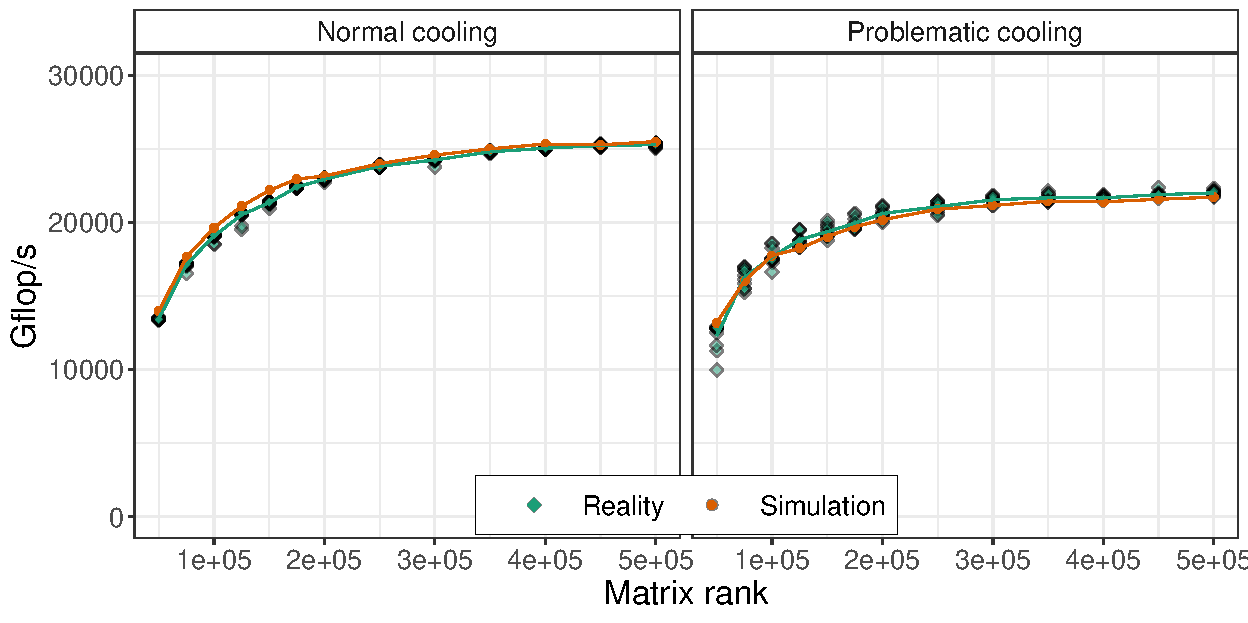
\includegraphics[width=\linewidth]{img/prediction/validation/temperature/validation_temperature.pdf}
            \end{minipage}%
            \begin{minipage}{0.2\linewidth}
                \scalebox{.8}{\begin{tabular}{l|l}
                $N$         & \Num{50000} \dots \Num{500000}               \\
                \texttt{NB}        & \Num{128}          \\
                \texttt{P}$\times$\texttt{Q}             & 32$\times$32        \\
                \texttt{PFACT}     & Crout         \\
                \texttt{RFACT}     & Right         \\
                \texttt{SWAP}      & Binary-exch.  \\
                \texttt{BCAST}     & 2 Ring        \\
                \texttt{DEPTH}     & 1             \\
                \end{tabular}}
            \end{minipage}
            \caption{HPL performance: predictions vs. reality (effect of the cooling issue on the nodes dahu-\{13,14,15,16\}).}
            \label{fig:validation_temperature}
        \end{figure}

        Our simulation approach makes it possible to predict the performance of HPL for a new platform state by merely
        making a new calibration whenever a significant change is detected.  This ability to reflect in simulation a
        platform change is illustrated in Figure~\ref{fig:validation_temperature} which, similarly to
        Figure~\ref{fig:validation_performance} (acquired in March 2019), showcases the influence of matrix size on the
        performance but at different periods.  The left plot represents the \emph{normal} state of the cluster (in
        September 2020), whereas the right plot has been obtained (in March-April 2019) when 4 of the 32 nodes had a
        cooling issue which lowered their performance by about \NSI{10}{\percent}. In all cases, we consistently predict
        performance within a few percent and performing a new \dgemm calibration on these four nodes was all
        that was needed to reflect this platform change in the simulation.
        This result illustrates both the faithfulness of our simulations and a potential use case for predictive
        simulations: a discrepancy between the reality and the predictions can sometimes indicate a real issue on the
        platform (similar situations have already been reported with SMPI\cite{smpi}).

    \section{Different geometries}%
    \label{sec:different_geometries}
        %% TODO - Validation de la géométrie. On arrive également à prédire pour toutes les
        %% géometries. Encore une fois, des difficultés (cette fois qu'on on utilise des
        %% géométries trés élongées, avec un petit P par exemple), voir section
        %% expérimentation.
        Figure~\ref{fig:validation_geometry} illustrates the influence on the performance of the geometry of the virtual
        topology (\texttt{P} and \texttt{Q}) used in HPL\@.  As expected, geometries that are too distorted lead to
        degraded performance.  All the HPL parameters were fixed (matrix rank is fixed to \Num{250000} and the other
        parameters are the same as in Section~\ref{sec:different_problem_sizes}) except for the geometry as we evaluate
        all the pairs (\texttt{P}, \texttt{Q}) such that \(\texttt{P}\times\texttt{Q}=960\).  We used only 30 nodes
        instead of 32 to cover a larger number of geometries, as \Num{960} has more divisors than \Num{1024}.

        \begin{figure}[htpb]
            \centering
            \subfigure[Illustrating the effect of the two MPI calibration methods. The optimistic method merely samples
            message size smaller than \SI{1}{\mega\byte} and extrapolates for larger sizes. Unfortunately, for messages
            larger than \SI{160}{\mega\byte}, the effective bandwidth significantly drops. The more realistic
            calibration measures MPI communication duration for messages up to \SI{2}{\giga\byte} while injecting some
            computation load in the background.  \label{fig:mpi_calibration}]{
                    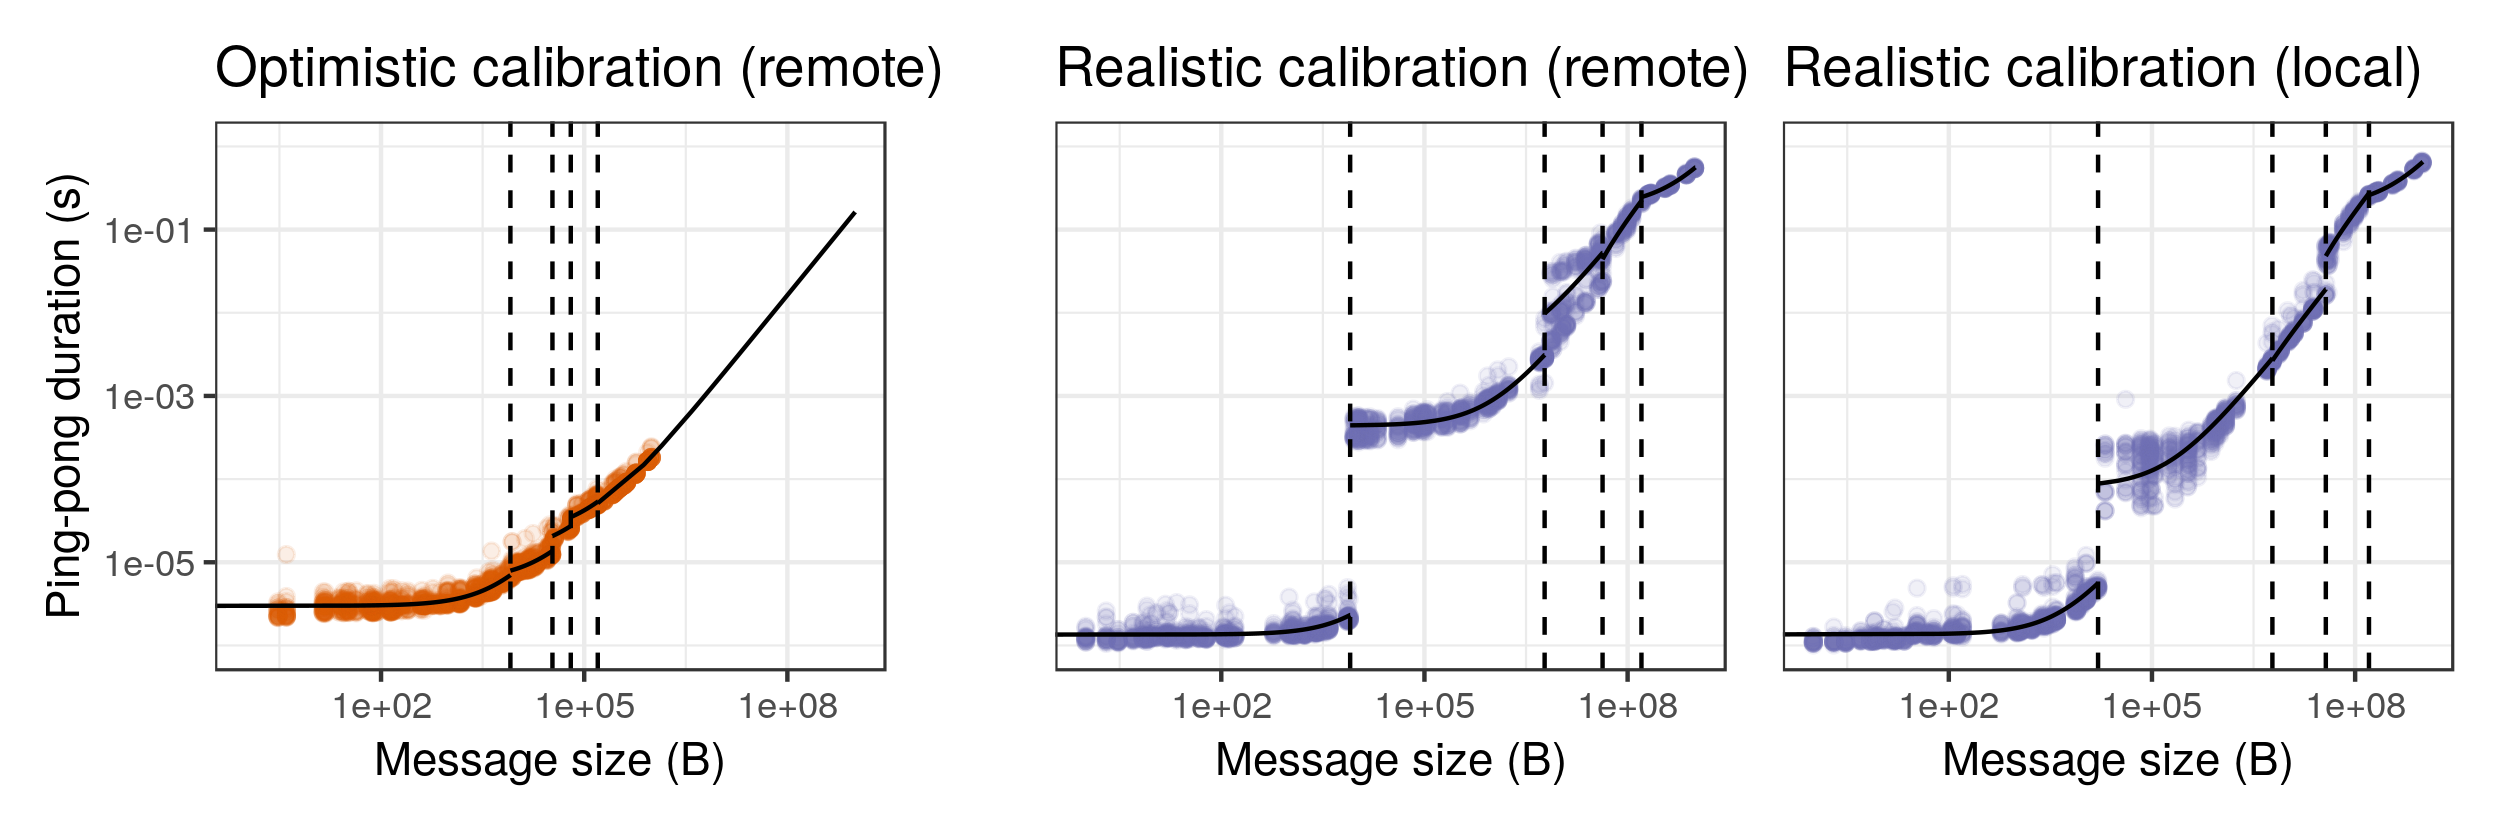
\includegraphics[width=\linewidth]{img/prediction/validation/mpi_calibration/mpi_calibration.png}
            }

            \subfigure[HPL performance: predictions vs. reality (testing all the
            possible geometries for 960 MPI ranks).\label{fig:validation_geometry}]{
                \begin{minipage}{0.8\linewidth}
                    \centering
                    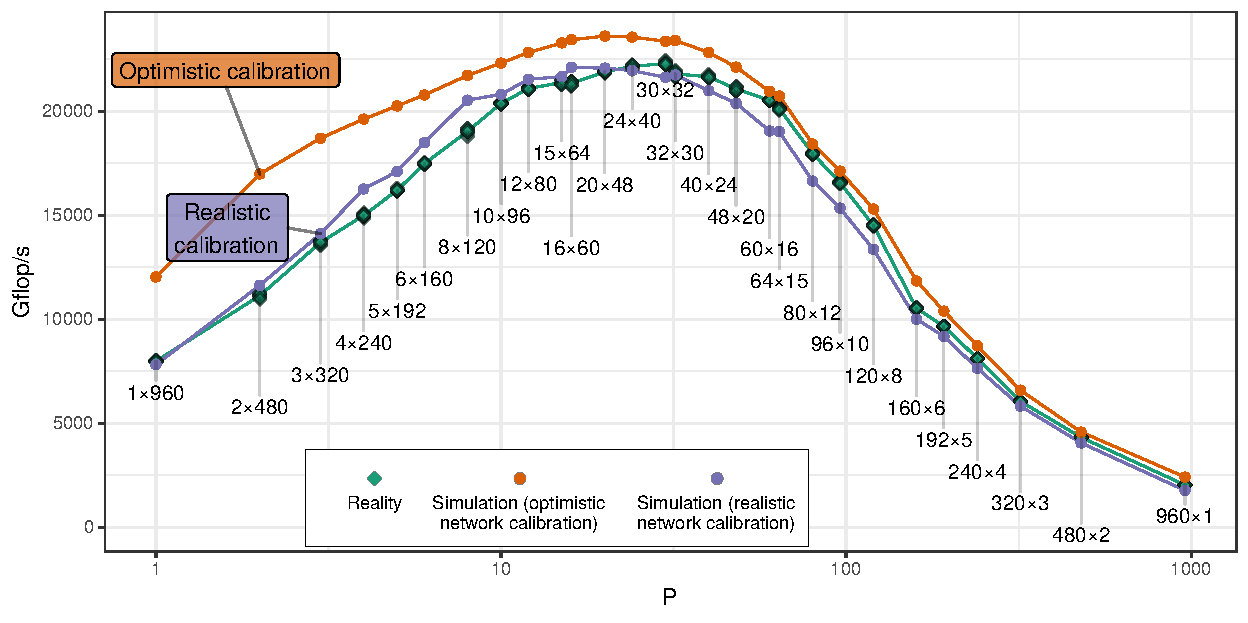
\includegraphics[width=\linewidth]{img/prediction/validation/geometry/validation_geometry.pdf}

                \end{minipage}%
                \begin{minipage}{0.2\linewidth}
                    \scalebox{.8}{\begin{tabular}{l|l}
                    \texttt{N}         & \Num{250000}               \\
                    \texttt{NB}        & \Num{128}          \\
                    \texttt{P}$\times$\texttt{Q}             & 960        \\
                    \texttt{PFACT}     & Crout         \\
                    \texttt{RFACT}     & Right         \\
                    \texttt{SWAP}      & Binary-exch.  \\
                    \texttt{BCAST}     & 2 Ring        \\
                    \texttt{DEPTH}     & 1             \\
                    \end{tabular}}
                \end{minipage}
            }
            \caption{The first (optimistic) network calibration gave poor
              predictions for very elongated geometries while the improved
              calibration provides perfect predictions.}
            \label{fig:validation_geometry_global}
        \end{figure}

        As in all our previous studies, we report both the predicted performance and the one measured in reality. Like
        the comparisons presented in the previous section, the simulation was done with the \dgemm model from
        Eq~\eqref{eq:dgemm.complex} (stochastic, heterogeneous, and polynomial) and the simplest linear models for the
        other kernels.  In our first simulation attempt that relied on a relatively simple network model (deterministic
        yet piecewise-linear to account for protocol switch) depicted on the leftmost plot of
        Figure~\ref{fig:mpi_calibration}, we obtained the unsatisfying orange line on top of
        Figure~\ref{fig:validation_geometry} for the prediction.  The simulations with the smallest value of \texttt{P}
        had relatively large prediction errors, with a systematic over-estimation that reaches up to +50\% for the
        \(1\times960\) and \(2\times480\) geometries.  A qualitative comparison of the execution traces obtained in
        reality and simulation showed that the broadcast phases' duration was greatly underestimated in simulation. We
        found out that with such elongated geometries, the message size is significantly larger than what we had used in
        our calibration, and the performance surprisingly and significantly drops for such size (compare with the
        rightmost plots of Figure~\ref{fig:mpi_calibration}). This performance drop is explained by poor optimization of
        the DMA locking mechanism in the Infiniband network layer\cite{denis:inria-00586015}. A similar performance drop
        also happens for intra-node communications that poorly manage the caches above a given size. Furthermore, the
        communication patterns generated by HPL during the ring broadcast are significantly impacted by the busy waiting
        of HPL that intensively calls \texttt{MPI\_Probe} and \dgemm on small sub-matrices. Our initial
        procedure for calibrating the network did not capture this phenomenon since we did not inject any additional CPU
        load. This problem is further discussed in Section~\ref{sec:beware_of_experimental_conditions}.

        We addressed this problem by improving our network calibration procedure: (1) we use a distinct model for local
        and remote calibrations, (2) we sample the message sizes in a larger interval, and (3) we add calls to \dgemm
        and \texttt{MPI\_Iprobe} between each call to \send and \recv. The goal was to make the calibration environment
        more similar to what happens in HPL\@.  The resulting network model is illustrated in the rightmost plots of
        Figure~\ref{fig:mpi_calibration}.  This more realistic network model solved every previous misprediction and
        allows us to produce very faithful simulations (purple line on Figure~\ref{fig:validation_geometry}), which are
        now a few percent of the reality regardless of the geometry.  This figure also illustrates the influence of the
        geometry on overall performance since there is almost a factor of ten between the worst configuration
        (\(960\times1\)) and the best one (\(30\times32\)). Although it is not surprising to see that the geometries
        which are as square as possible lead to better performance as they minimize the overall amount of data
        movements, it is interesting to observe the asymmetric role of \texttt{P} and \texttt{Q} in the overall
        performance (smaller values for \texttt{P} lead to better performance) and which can be explained by the
        structure of the collective operations but requires a close look at the code.

    \section{Factorial experiment}%
    \label{sec:factorial_experiment}
        %% TODO On arrive à prédire pour toutes les configurations de paramètres.
        %% Plusieurs difficultés (cf. section expérimentation).

        Although geometry is among the most important parameter to tune, six other parameters control the behavior of
        HPL. In Figure~\ref{fig:validation_factorial}, we compare the performance reported by HPL when fixing the matrix
        rank to \Num{250000} and varying the following parameters: block size (128 or 256), depth (0 or 1), broadcast
        (the six available algorithms), swap (the three available algorithms). The geometry was fixed to
        \(\text{P}\times\text{Q}=32\times32=1024\) as it is optimal (the simpler calibration procedure and the network
        model depicted on the leftmost plot of Figure~\ref{fig:mpi_calibration} were thus used). The parameters
        \texttt{pfact} and \texttt{rfact} (panel factorization) were respectively fixed to \texttt{Crout} and
        \texttt{Right}, as they had nearly no influence on HPL performance in our early experiments.

        \begin{figure}[htpb]
            \centering
            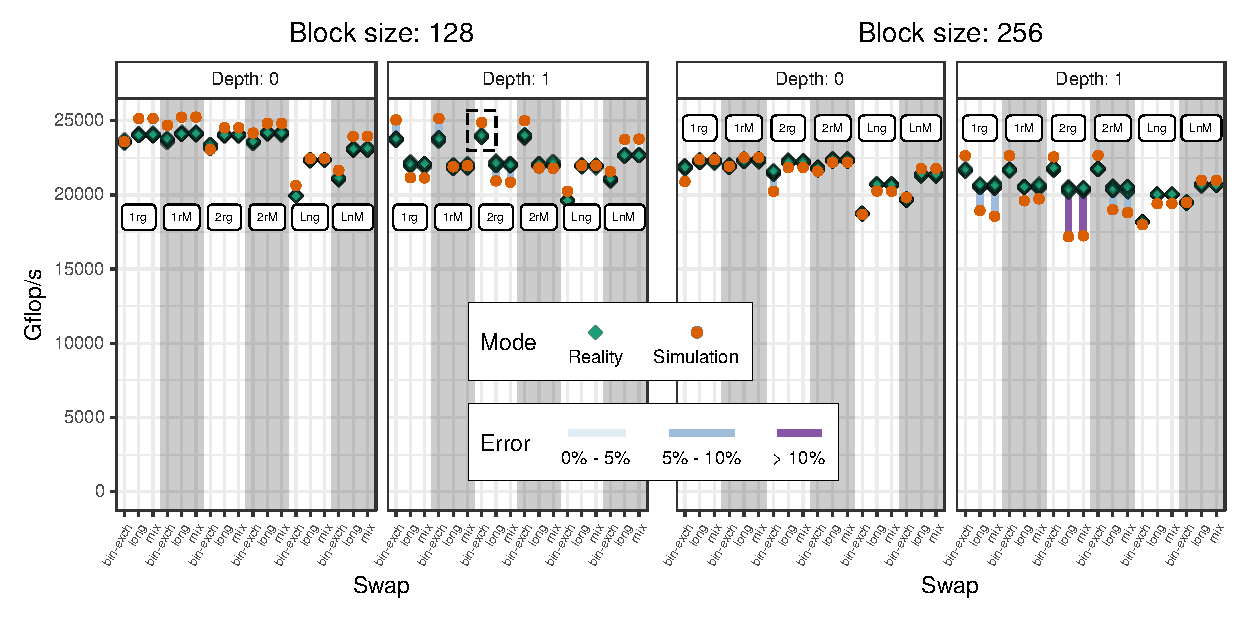
\includegraphics[width=\linewidth]{img/prediction/validation/factorial/validation_factorial.pdf}
            \caption{Influence of HPL configuration on the performance (factorial experiment). Parameters have been
                reorganized based on their influence on performance to improve readibility. The boxed configuration
                corresponds to the one boxed in Figure~\ref{fig:validation_performance}.
            }
            \label{fig:validation_factorial}
        \end{figure}

        Figure~\ref{fig:validation_factorial} depicts the 72 parameter combinations we tested. These parameters account
        for up to \SI{30}{\percent} of variability in the performance, which is less important than the geometry but is
        still quite significant. For 61 of them, the prediction error is lower than \SI{5}{\percent}. Only two
        combinations have shown a large error of approximately \SI{15}{\percent}, obtained with a block size of 256, a
        depth of 1, the \texttt{2-ring} broadcast algorithm, and either the \texttt{long} or the \texttt{mix} swap
        algorithm. This demonstrates the soundness of our approach, as our predictions are reasonably accurate most of
        the time.  This experiment confirms that, although the prediction of HPL performance for a given parameter
        combination has a systematic bias, the error remains within a few percent most of the time. Therefore, this
        surrogate is good enough for parameter tuning and should be considered when preparing a large-scale run.

        While testing all the parameter combinations is the safest method to discover the combination that provides the
        highest performance, its cost can be prohibitive due to the high number of combinations. An alternative often
        used in practice is to explore only a small subset of the parameter space and to analyze variance (ANOVA) to
        identify the parameters with the more substantial effect on performance and then select the appropriate
        combination.  We applied this procedure on samples of both datasets (the one obtained from real runs and the one
        obtained in simulation). In both cases, the two parameters with the highest effect were the block size
        \texttt{NB} and the \texttt{depth}, as shown in Figure~\ref{fig:validation_factorial}, followed by
        \texttt{bcast} and \texttt{swap}. The best combinations selected in both cases were also identical,
        demonstrating once again the faithfulness of our simulation approach and how it can be used to reduce the
        experimental cost of parameter tuning.

    \section{Conclusion}%
        %% TODO - Un travail de fourmi et d'expert. Plusieurs difficultés:
        %% - être sûr que le simulateur fait bien ce qu'on veut (pas mal de paramètres "magiques")
        %% - cf. section expérimentation
        Accurately predicting the performance of an application is not a trivial task. Discrepancies between reality and
        simulation can be multiple: the platform may have changed (\eg the cooling issue that affected four nodes in
        Section~\ref{sec:platform_change}), the model could be inaccurate (\eg the homogeneous and deterministic \dgemm
        model is too simple as in Section~\ref{sec:different_problem_sizes}) or not correctly calibrated (\eg the
        calibration procedure does not cover the appropriate parameter space, or the experimental conditions are too
        different as in Section~\ref{sec:different_geometries}). As expected in any serious investigation of model
        validity, our validation study is not a mere collection of positive cases. Instead, it is the result of a
        thorough (we extensively covered the HPL parameter space) attempt to invalidate our model as well as
        explanations on how we did so. By meticulously overcoming each of these issues, we have demonstrated the ability
        of our approach to produce very faithful predictions of HPL performance on a given platform.

        The difficulties encountered while conducting experiments will be discussed more thoroughly in
        Part~\ref{part:experiment}.

\chapter{Sensibility analysis}%
\label{chapter:prediction:sensibility}
    %% TODO Tentative de réponse à toutes les questions (farfelues ou pas) qu'on a
    %% pu se poser autour d'HPL mais auxquelles on n'a jamais pu répondre
    %% avec des expériences réelles...

    %% TODO Reprendre le petit rapport que j'avais rédigé sur l'étude théorique de la suppression de noeuds lents:
    %% /home/tom/Documents/Fac/phd/reports/2020/node_removal
    %% Également ma tentative de modélisation de la performance de HPL en fonction de P et Q avec un modèle linéaire
    %% (échec, ce qui montre la difficulté de la chose).


    We have shown that many typical HPL case studies could be conducted in simulation. However, their conclusions
    (optimal geometry and parameters) are specific to the cluster we used and they require a precise model of several
    aspects of the target cluster, which may not be possible at early experimental stages. In particular, only a few
    cluster nodes may be available at first and the whole cluster model should then be constructed from a limited set of
    observations and carefully extrapolated. This section shows how typical \emph{what-if} simulation studies should be
    conducted given such uncertainty. We have presented in Section~\ref{sub:dgemm_model:generative_models} a generative
    model of node performance that can easily be fit from daily measurements and used to produce a similar platform.
    This model is used to quantify the importance on overall performance of temporal variability of the \dgemm kernel in
    Section~\ref{sec:influence_of_temporal_variability} and of spatial variability of nodes in
    Section~\ref{sec:influence_of_spatial_variability}. In particular, we show how to study the efficiency of a simple
    \emph{slow node eviction} strategy. Finally, we study in Section~\ref{sec:influence_of_physical_topology} the
    influence of the physical network topology on overall performance. Most of these studies are particularly difficult
    to conduct through real experiments because of the difficulty to finely control the platform.

    \section{Influence of \dgemm temporal variability}%
    \label{sec:influence_of_temporal_variability}
        In Section~\ref{sec:different_problem_sizes}, we could highlight the importance of accounting for temporal
        variability of the \dgemm kernel to obtain faithful HPL predictions. To the best of our knowledge, HPL
        developers and experts are often aware of this influence (or at least suspect it). However, they have never
        fully quantified it since designing and performing real experiments to evaluate this would be quite difficult.
        Although increasing this variability wouldn't be too hard, reducing it would be particularly complicated. This
        can however easily be done through simulation using the hierarchical model of the previous section. In our
        experiments, the order of magnitude of the temporal variability with respect to actual performance (i.e., the
        ratio between \(\gamma_{p,d}\) and \(\alpha_{p,d}\) in Equation~\eqref{eq:dgemm.basic}) was around
        \NSI{3}{\percent}. This may be a ``normal'' value or could be considered too high and possibly improved by
        better controlling thread mapping or Operating System noise. Such a task can be quite tedious and knowing how
        much performance gain can be expected beforehand is thus quite useful. In this section, we study the influence
        of this variability by generating 10 cluster scenarios using the previous model (as in Figure~\ref{fig:whatif}),
        comprising \Num{1024} nodes each, but by constraining \(\gamma_{p,d}\) to be equal to \(\gamma.\alpha_{p,d}\)
        with \(\gamma\in[0,0.1]\), which represents the coefficient of variation of the \dgemm kernel. We evaluate the
        performance of HPL with one multi-threaded MPI rank per node, a block size of 512, a look-ahead \texttt{depth}
        of 1.  We used the \texttt{increasing-2-ring} broadcast with the \texttt{Crout} panel factorization algorithms
        and \(\texttt{P}\times\texttt{Q}=8\times32\) and we tested matrix sizes ranging from 100,000 to 500,000. Let us
        denote by \(T(N,C_i,\gamma)\) the performance of HPL when factorizing a matrix of rank \(N\) on cluster \(C_i\)
        with a temporal variability of \(\gamma\). The overhead for this configuration is the ratio

        \begin{equation*}
            O(N,C_i,\gamma) = \frac{\mathbb{E}[T(N,C_i,\gamma)]}{T(N,C_i,0)}-1.
        \end{equation*}

        \begin{figure}[htpb]
            \centering
            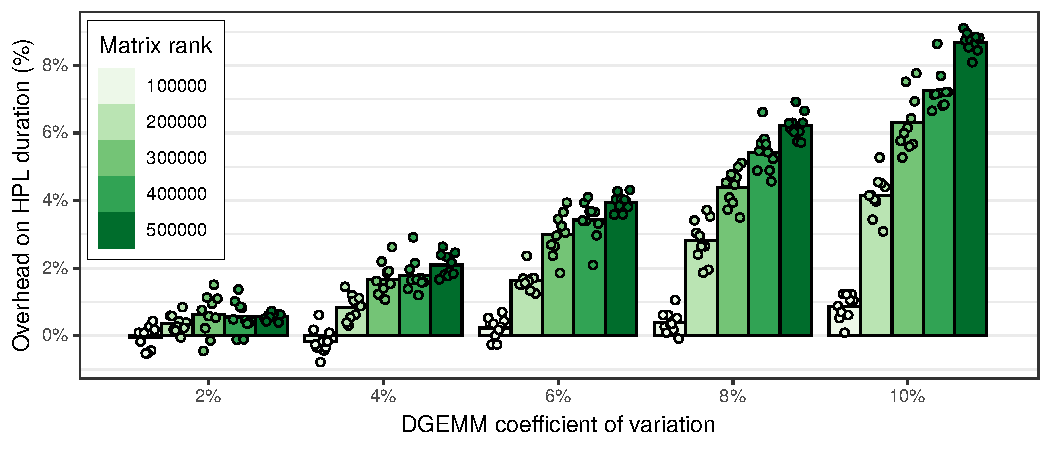
\includegraphics[width=\linewidth]{img/prediction/sensibility/temporal/whatif_variability.pdf}

            \caption{The overhead on HPL duration appears to be linear in \dgemm temporal variability. Although
            it is negligible for small matrices, it severely inflates for larger matrices.}
            \label{fig:whatif_variability}
        \end{figure}

        Each bubble in Figure~\ref{fig:whatif_variability} represents one such overhead. For any \(\gamma\), this
        overhead appears to be negligible for small matrices and to increase and flatten when \(N\) grows large. In most
        TOP5000 qualification runs, the matrix is made as large as possible and the overhead would thus appear to grow
        roughly linearly with \(\gamma\). On a new cluster, a simple statistical evaluation of the nodes' performance
        using the model of Section~\ref{sub:dgemm_model:generative_models} would thus be a good first diagnosis of
        whether trying to decreasing temporal variability is a promising tuning target or not.

    \section{Influence of \dgemm spatial variability}%
    \label{sec:influence_of_spatial_variability}
        Although we showed in Section~\ref{sec:different_problem_sizes} that temporal variability could account for
        about \NSI{9}{\percent} of performance, spatial variability was even more important as it was responsible for
        \NSI{22}{\percent} of overhead compared to a fully homogeneous cluster. In practice, the replacement of a few
        nodes may be possible but such spatial variability is expected and common\cite{rountree_15} and a workaround
        would have to be found. A common approach consists in dropping out a few of the slowest nodes. Indeed, since the
        matrix is evenly divided between the nodes, the computation inevitably progresses at the speed of the slowest
        node. However, removing the slowest nodes also decreases the overall processing capability and impacts the
        virtual topology's geometry (the \texttt{P} and \texttt{Q} parameters of HPL). Such adjustment is often done by
        trial and error and is all the more tricky as temporal variability and uncertainty from real experiments come
        into play. In this section, we show how such a subtle trade-off can be studied in simulation.

        \begin{figure}[htpb]
            \centering
            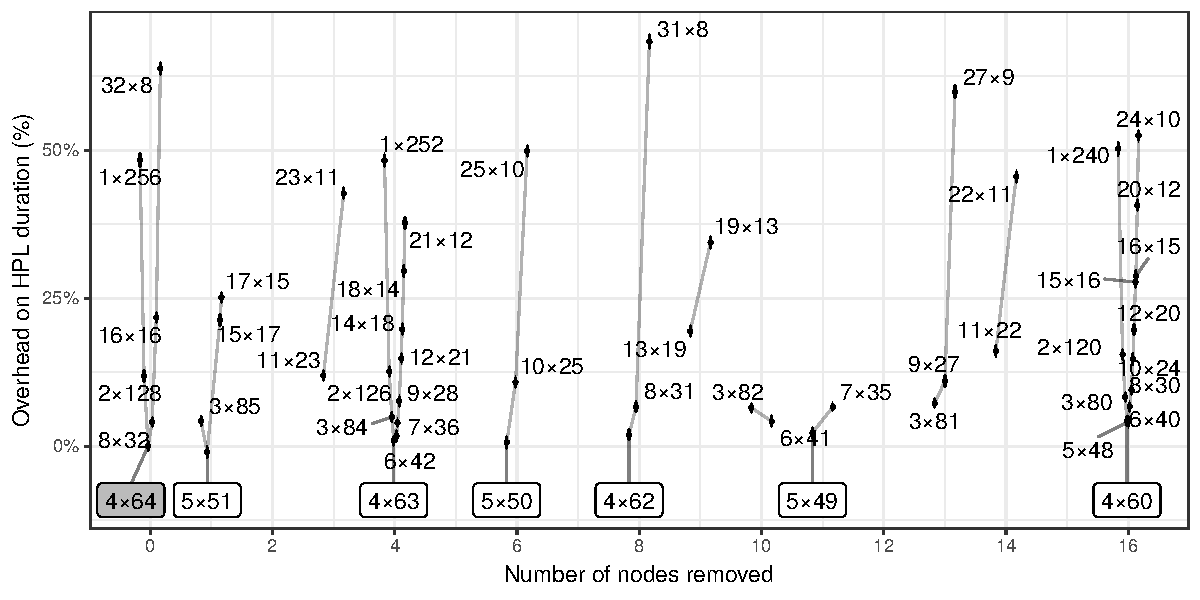
\includegraphics[width=\linewidth]{img/prediction/sensibility/spatial/whatif_removing_nodes.pdf}
            \caption{Influence of the number of nodes on the performance of HPL\@. The geometry of the virtual topology
                is particularly influent and it appears that $\mathtt{P}\times\mathtt{Q}$ configurations with a small
                $\mathtt{P}$ perform significantly better then those with a larger $\mathtt{P}$. Each configuration is
                summarized through the average overhead over the 10 clusters and errorbars represent a 95\% confidence
            interval.}
            \label{fig:whatif_removing_nodes}
        \end{figure}

        Using the model from Section~\ref{sub:dgemm_model:generative_models}, we generate 10 mildly heterogeneous 256
        node clusters (i.e., where nodes are similar to the ones of our cluster when operating in the normal state as in
        Figure~\ref{fig:whatif_calibration}) and we study the performance obtained when removing 1 to 16 of the slowest
        nodes. When removing nodes, the geometry should be adjusted depending on how the number of remaining nodes
        decomposes in prime factors. As observed in Figure~\ref{fig:validation_geometry}, having \texttt{P} \(\approx\)
        \texttt{Q} is generally a good idea to reduce the total amount of communication. However it may be
        counter-productive for a given broadcast or swap algorithm that serializes communications.
        Figure~\ref{fig:whatif_removing_nodes} shows the average (over the 10 clusters) overhead for a matrix of rank
        \Num{250000} compared to the best performance obtained using the whole cluster. We group the different
        \(\texttt{P}\times\texttt{Q}\) decompositions and order them by increasing \texttt{P}. Again, we use the
        \texttt{2-Ring} and \texttt{Binary-exch} algorithms, which are among the best configurations according to the
        study of Section~\ref{sec:factorial_experiment}. It appears that the \(4\times64\) geometry now achieves the
        best trade-off between the total amount of communications and how well they overlap with each other. The optimal
        configuration for each number of nodes is boxed in Figure~\ref{fig:whatif_removing_nodes}. It reveals that there
        is not much to gain, probably because of the mild spatial heterogeneity of our cluster, but that optimizing the
        virtual topology is particularly important.

        \begin{figure}[htpb]
            \centering
            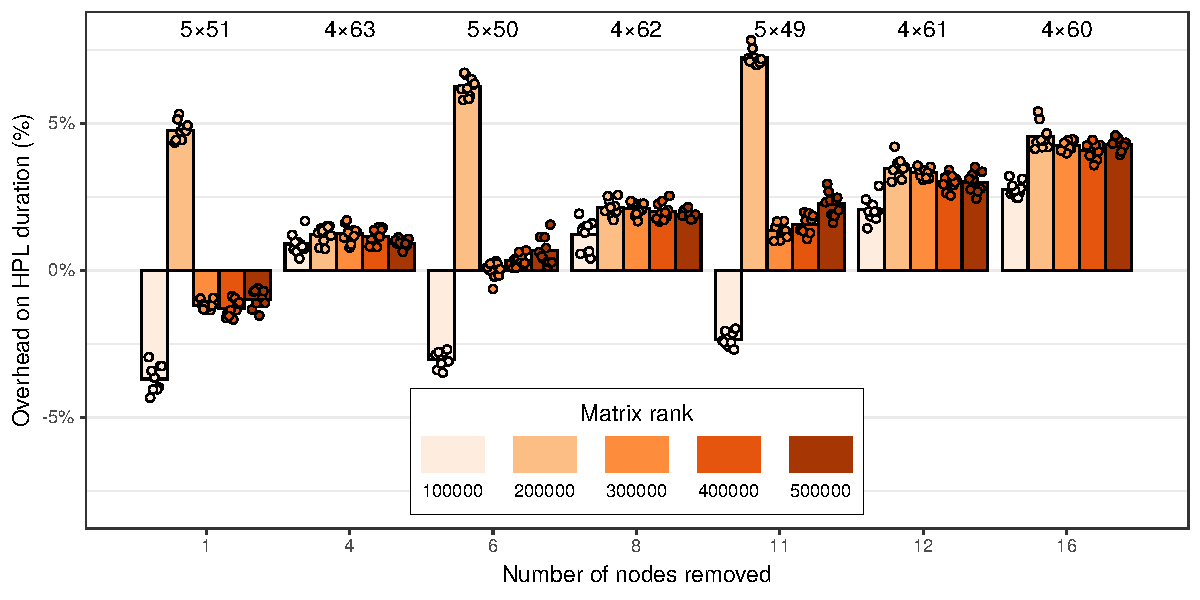
\includegraphics[width=\linewidth]{img/prediction/sensibility/spatial/whatif_removing_nodes_2.pdf}
            \caption{Influence of node removal on performance while taking into account the matrix rank. Due to the mild
            heterogeneity of these scenarios, evicting nodes brings no benefit.}
            \label{fig:whatif_removing_nodes_2}
        \end{figure}

        Figure~\ref{fig:whatif_removing_nodes_2} investigates how this overhead for the best geometry and node selection
        also depends on the matrix rank. It appears that in this scenario, except for very small matrices, removing
        nodes cannot help improving performance. Note that the overhead for \(5\times\texttt{Q}\) configurations with a
        matrix rank 200,000 appears to behave differently from what happens for other matrix sizes. This surprising
        effect probably arises from a subtle combination of matrix size and virtual topology. We could indeed observe on
        our cluster that such configurations had a weakly but significantly worse performance than the other
        configurations. Such interaction also explains why designing a faithful analytical model of HPL is so difficult
        and why a full simulation of the whole application is generally required.  Although absolute performance should
        be taken with a grain of salt when studying such subtle effects, they are easily overlooked when conducting real
        experiments. In this particular small scale mild heterogeneity scenario, there is thus no gain in removing nodes
        but, as illustrated in Figure~\ref{fig:whatif_removing_nodes_heterogeneous} where we used a multimodal spatial
        heterogeneity (as in Figure~\ref{fig:whatif_slow}), this may be a relevant approach.  This sensibility analysis
        shows how, for a given supercomputer, a simple statistical evaluation of the spatial heterogeneity allows
        evaluating whether spatial variability is a promising tuning target or not.

        \begin{figure}[!t]
            \centering
            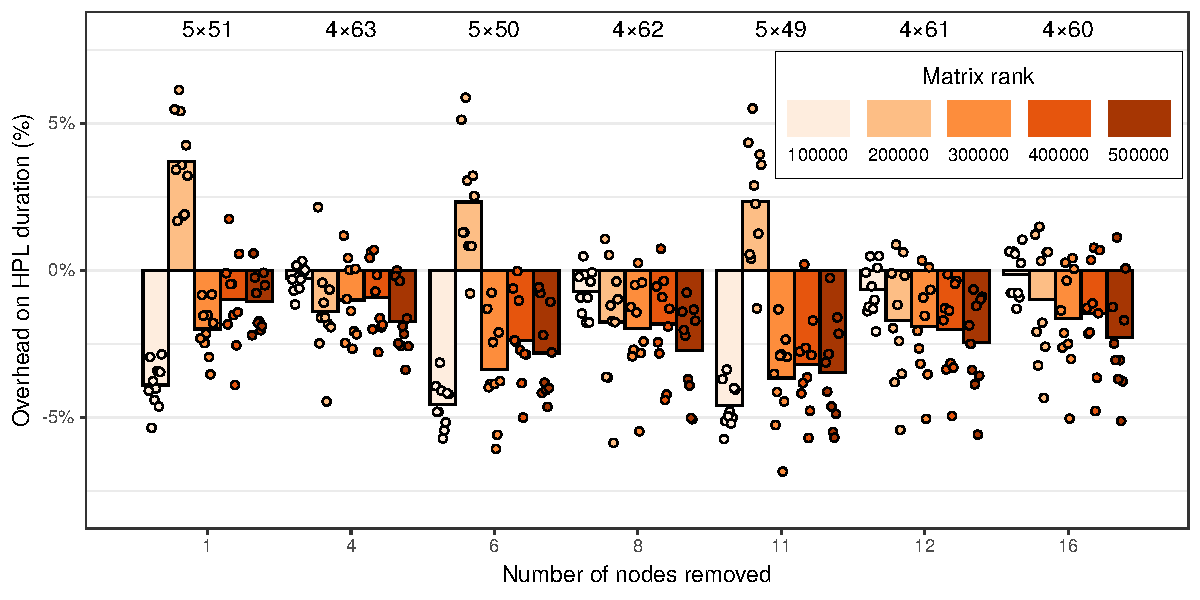
\includegraphics[width=\linewidth]{img/prediction/sensibility/spatial/whatif_removing_nodes_2_heterogeneous.pdf}
            \caption{Influence of node removal on performance in a stronger heterogeneity scenario (extrapolation of our
            test cluster when it had a cooling problem on 4 of its nodes). Removing 6 to 12 nodes our of 256 nodes may
            bring substential improvement and such optimization would therefore be worth investigating.}
            \label{fig:whatif_removing_nodes_heterogeneous}
        \end{figure}

    \section{Influence of the physical topology}%
    \label{sec:influence_of_physical_topology}

        Finally, since virtual topology and communications appear to significantly influence the overall performance,
        one may wonder how much the physical topology influences the performance. Indeed, several recent
        articles\cite{tapered_fat_tree_16,tapered_fat_tree_19} report that interconnect networks are often oversized
        compared to the actual need of applications and that turning off some switches could sometimes go completely
        unnoticed by end-users. In this section we consider ten 256 node clusters with variable node performance (as in
        Figure~\ref{fig:whatif}) interconnected by a 2-level fat-tree and quantify by how much performance degrades when
        the top-tier switches are gradually deactivated. More formally, we use a \texttt{(2;32,8;1,N;1,8)} fat-tree with
        \(\texttt{N}\in\{1,2,3,4\}\).

        \begin{figure}[htpb]
            \centering
            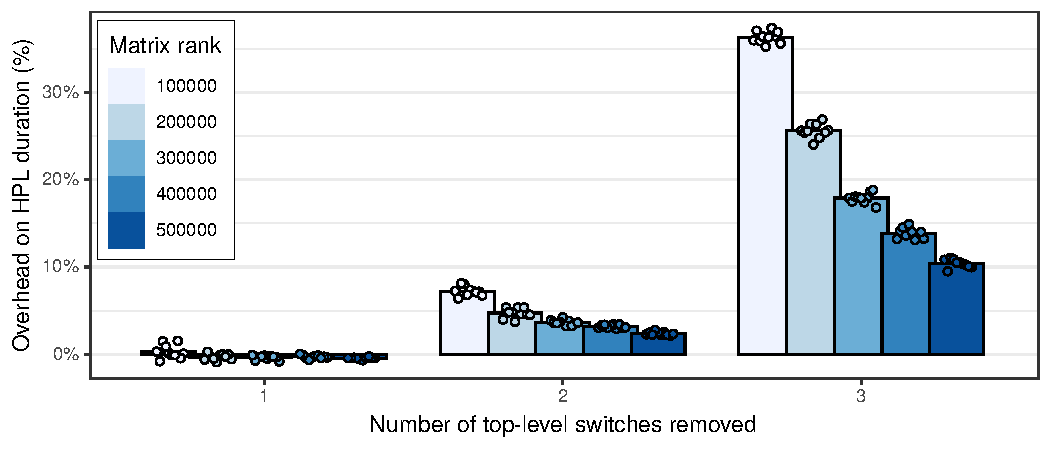
\includegraphics[width=\linewidth]{img/prediction/sensibility/topology/whatif_removing_switches.pdf}

            \caption{Influence of the physicical topology on the overall performance. It is possible to remove up to 2
            of the top-level switches without significantly hurting performances for large matrices. Beyond this point,
            communications become the main performance bottleneck.}
            \label{fig:whatif_removing_switches}
        \end{figure}

        Figure~\ref{fig:whatif_removing_switches} depicts this degradation as a function of matrix size. As one could
        expect, the impact is more significant for smaller matrix sizes (where the execution is more network bound).
        Although removing one switch leads to absolutely no visible performance loss, removing two or three switches can
        have a dramatic effect. Again, such degradation depends on the broadcast and swap algorithms and may be slightly
        mitigated. To the best of our knowledge, it is the first time such sensibility analysis is conducted faithfully.
        Generating random node configurations allows avoiding potential bias, in particular against perfectly
        homogeneous scenarios. We believe such a tool can be quite useful in the earlier steps of a supercomputer design
        when performing capacity planning to adjust the network capacity to a given cost and power envelope.
